% =========================================================================
% 《高中數學實驗教材》第三冊（自然組）
% 第三章 向量幾何的基礎及其代數的運算體系
% 依據 1975 年再版教材掃描原件（pp. 71-128）高高保真轉錄
% =========================================================================

\section{向量幾何的基礎及其代數的運算體系}
\label{sec:b3-ch3}

\subsection*{本章大綱與導言}

\begin{itemize}[leftmargin=3em]
  \item[§3-1] 點的座標與距離
  \item[§3-2] 從各種觀點看向量
    \begin{itemize}[leftmargin=2em]
      \item[甲、] 幾何觀點——相對位置的觀點
      \item[乙、] 向量、點與座標
      \item[丙、] 移動觀點
      \item[丁、] 力學觀點
    \end{itemize}
  \item[§3-3] 向量的加減法
    \begin{itemize}[leftmargin=2em]
      \item[甲、] 向量加法的幾何意義
      \item[乙、] 向量加法的基本性質
      \item[丙、] 向量的分解與加法的座標成分表示
      \item[丁、] 向量的減法
    \end{itemize}
  \item[§3-4] 向量的係數積
    \begin{itemize}[leftmargin=2em]
      \item[甲、] 係數積的幾何意義
      \item[乙、] 係數積的座標成分表示
      \item[丙、] 係數積的基本性質
    \end{itemize}
  \item[§3-5] 向量的內積
    \begin{itemize}[leftmargin=2em]
      \item[甲、] 單位向量與向量的自然分解
      \item[乙、] 內積
      \item[丙、] 內積的座標成分表示
      \item[丁、] 內積的分配律
      \item[戊、] 向量處理的例子
    \end{itemize}
  \item[§3-6] 利用內積導出三角和角公式
  \item[§3-7] 行列式與面積、體積
\end{itemize}

\begin{center}
* \qquad\qquad * \qquad\qquad * \qquad\qquad * \qquad\qquad *
\end{center}

§3-1 利用座標表示平面或空間中兩點距離.

§3-2 以相對位置，移動及力學三種觀點來解釋向量的內涵，而著重在第一種觀點，強調向量、發自原點的有向線段與點三者間的對應關係，而導出用座標成分來描述向量的想法.

§3-3, §3-4, §3-5 分別討論向量的代數運算：加減、係數積與內積.（外積也是一種很重要的運算，不過目前暫且不講.）在這些運算中，我們一方面把向量本身的幾何意義顯示出來，另一方面導出以向量座標成分表示的代數式. 尤其對內積，我們特別強調這樣的對照，這對照使我們知道在幾何的要求下，什麼時候，怎樣利用向量的代數結構，利用向量座標成分的表示來作為我們演算的工具. 在這幾節裏，我們已開始利用剛引入的向量運算處理古典平面幾何的問題，同時也作了一些應用. 這些便是向量幾何的實質. 在 §3-6，我們利用向量證明三角函數的和角公式.

§3-7 最後一節，以向量的座標成分，討論二階行列式代表面積的幾何意義. 對三階行列式代表體積的幾何意義，我們也提了出來，但未加證明.

% =========================================================================
% § 3-1 點的座標與距離
% =========================================================================
\subsection{點的座標與距離}
\label{sec:b3-3-1}

第一章介紹座標幾何（§1-2）時，為了以實數對來描寫平面上的點，曾藉助一任意取定的原點 $O$ 及相互垂直的 $X, Y$ 兩軸，這樣的原點 $O$ 及 $X, Y$ 兩軸便稱為一個平面的直角座標系，記為 $(O; X, Y)$.

接著我們談到：如何根據一個取定的直角座標系 $(O; X, Y)$ 把平面上的點 $A$ 轉化成實數對 $(x, y)$，這個 $(x, y)$ 就稱為 $A$ 點相關於直角座標系 $(O; X, Y)$ 的座標，或簡稱為 $A$ 的座標，其中 $x$ 與 $y$ 稱為 $A$ 點座標的兩個成分，常簡記為 $A(x, y)$.

同樣對於空間，我們取定原點 $O$，及通過 $O$ 且相互垂直的三個軸 $X, Y, Z$. 稱它們構成一個空間的直角座標系，記為 $(O; X, Y, Z)$. 這樣，空間中的點 $A$ 就可以用 $(x, y, z)$ 來描寫，見圖 3-1. 此時 $(x, y, z)$ 就稱為 $A$ 點相關於直角座標系 $(O; X, Y, Z)$ 的座標，或簡稱為 $A$ 的座標. 其中 $x, y$ 與 $z$ 稱為 $A$ 點座標的三個成分，常簡記為 $A(x, y, z)$.

\begin{figure}[H]
\centering
\begin{minipage}{0.55\textwidth}
\centering
\begin{tikzpicture}[>=stealth, scale=0.9, font=\small]
  % Axes
  \draw[->, thick] (0, 0) -- (-2, -1.8) node[below left] {$X$};
  \draw[->, thick] (0, 0) -- (3.5, 0) node[right] {$Y$};
  \draw[->, thick] (0, 0) -- (0, 3.2) node[above] {$Z$};
  \node[above left] at (0, 0) {$O$};

  % Coordinates of A
  % X-proj A1 on X axis, Y-proj A2 on Y axis
  \coordinate (A1) at (-0.8, -0.72);
  \coordinate (A2) at (1.8, 0);
  \coordinate (Aprime) at (1.0, -0.72);
  \coordinate (A) at (1.0, 1.3);

  \draw[dashed] (A1) -- (Aprime) node[midway, below] {$y$} -- (A2);
  \draw[dashed] (0, 0) -- (Aprime);
  \draw[dashed] (Aprime) -- (A) node[midway, right] {$z$};
  \draw[dashed] (0, 2.02) -- (A);
  \draw[very thick] (0, 0) -- (A);

  \fill (A) circle (1.5pt) node[above right] {$A(x, y, z)$};
  \fill (Aprime) circle (1.2pt) node[below right] {$A'$};
  \fill (A1) circle (1.2pt) node[left] {$A_1$};
  \fill (A2) circle (1.2pt) node[above right] {$A_2$};
  \node[left] at (-0.4, -0.36) {$x$};
\end{tikzpicture}
\caption{空間直角座標系中的點}
\label{fig:b3-fig3-1}
\end{minipage}
\hfill
\begin{minipage}{0.4\textwidth}
\centering
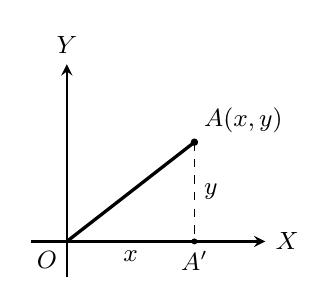
\begin{tikzpicture}[>=stealth, scale=0.9, font=\small]
  \draw[->, thick] (-0.5, 0) -- (2.8, 0) node[right] {$X$};
  \draw[->, thick] (0, -0.5) -- (0, 2.5) node[above] {$Y$};
  \node[below left] at (0, 0) {$O$};

  \coordinate (A) at (1.8, 1.4);
  \coordinate (Aprime) at (1.8, 0);

  \draw[dashed] (A) -- (Aprime);
  \draw[very thick] (0, 0) -- (A);

  \fill (A) circle (1.5pt) node[above right] {$A(x, y)$};
  \fill (Aprime) circle (1.2pt) node[below] {$A'$};

  \node[below] at (0.9, 0) {$x$};
  \node[right] at (1.8, 0.7) {$y$};
\end{tikzpicture}
\caption{平面直角座標系中的點}
\label{fig:b3-fig3-2}
\end{minipage}
\end{figure}

有了直角座標，便能把兩點間的距離以座標清楚地表示出來：先考慮平面的情形. 設在平面上相關於一直角座標系 $(O; X, Y)$，有一點 $A(x, y)$，則 $A$ 與原點 $O$ 的距離 $\overline{OA}$ 可由畢氏定理直接求得：
\[ \overline{OA}^2 = \overline{OA_1}^2 + \overline{A_1 A}^2 = x^2 + y^2, \]
故
\[ \overline{OA} = \sqrt{x^2 + y^2}. \]

若平面上有兩點 $P(x_1, y_1), Q(x_2, y_2)$，則 $P, Q$ 之間的距離（以後要簡稱為兩點的間距）基本上還是由畢氏定理來求算：

注意線段 $PQ$ 在 $X, Y$ 軸上投影的長度分別為 $|x_2 - x_1|, |y_2 - y_1|$ 故由畢氏定理：
\[ \overline{PQ}^2 = |x_2 - x_1|^2 + |y_2 - y_1|^2 \quad \text{〔圖 3-3 中，$\overline{PQ}^2 = \overline{PR}^2 + \overline{RQ}^2$〕} \]
即
\[ \overline{PQ} = \sqrt{|x_2 - x_1|^2 + |y_2 - y_1|^2}. \]

\begin{figure}[H]
\centering
\begin{minipage}{0.48\textwidth}
\centering
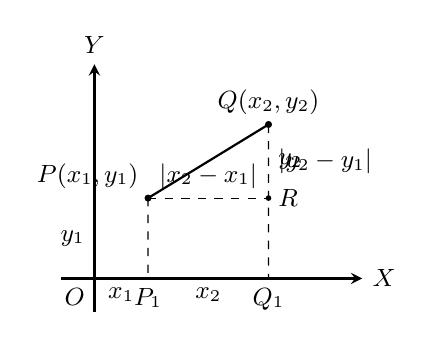
\begin{tikzpicture}[>=stealth, scale=0.85, font=\small]
  \draw[->, thick] (-0.5, 0) -- (4, 0) node[right] {$X$};
  \draw[->, thick] (0, -0.5) -- (0, 3.2) node[above] {$Y$};
  \node[below left] at (0, 0) {$O$};

  \coordinate (P) at (0.8, 1.2);
  \coordinate (Q) at (2.6, 2.3);
  \coordinate (R) at (2.6, 1.2);

  \draw[thick] (P) -- (Q);
  \draw[dashed] (P) -- (R) node[midway, above] {$|x_2 - x_1|$};
  \draw[dashed] (Q) -- (R) node[midway, right] {$|y_2 - y_1|$};

  \draw[dashed] (P) -- (0.8, 0) node[below] {$P_1$};
  \draw[dashed] (Q) -- (2.6, 0) node[below] {$Q_1$};

  \fill (P) circle (1.5pt) node[above left] {$P(x_1, y_1)$};
  \fill (Q) circle (1.5pt) node[above] {$Q(x_2, y_2)$};
  \fill (R) circle (1.2pt) node[right] {$R$};

  \node[below] at (0.4, 0) {$x_1$};
  \node[below] at (1.7, 0) {$x_2$};
  \node[left] at (0, 0.6) {$y_1$};
  \node[right] at (2.6, 1.75) {$y_2$};
\end{tikzpicture}
\caption{兩點間距離（第一象限情形）}
\label{fig:b3-fig3-3-1}
\end{minipage}
\hfill
\begin{minipage}{0.48\textwidth}
\centering
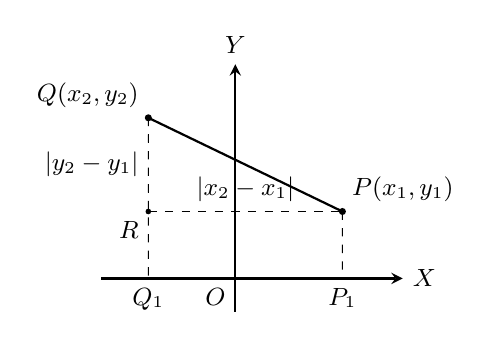
\begin{tikzpicture}[>=stealth, scale=0.85, font=\small]
  \draw[->, thick] (-2, 0) -- (2.5, 0) node[right] {$X$};
  \draw[->, thick] (0, -0.5) -- (0, 3.2) node[above] {$Y$};
  \node[below left] at (0, 0) {$O$};

  \coordinate (Q) at (-1.3, 2.4);
  \coordinate (P) at (1.6, 1.0);
  \coordinate (R) at (-1.3, 1.0);

  \draw[thick] (P) -- (Q);
  \draw[dashed] (R) -- (P) node[midway, above] {$|x_2 - x_1|$};
  \draw[dashed] (Q) -- (R) node[midway, left] {$|y_2 - y_1|$};

  \draw[dashed] (Q) -- (-1.3, 0) node[below] {$Q_1$};
  \draw[dashed] (P) -- (1.6, 0) node[below] {$P_1$};

  \fill (P) circle (1.5pt) node[above right] {$P(x_1, y_1)$};
  \fill (Q) circle (1.5pt) node[above left] {$Q(x_2, y_2)$};
  \fill (R) circle (1.2pt) node[below left] {$R$};
\end{tikzpicture}
\caption{兩點跨象限間距離}
\label{fig:b3-fig3-3-2}
\end{minipage}
\end{figure}

空間的情形也是一樣. \phantomsection\label{note:b3-ch3-p74-space-font}%
設在空間\footnote{【校訂註】原書此處排印鉛字損缺，字形作「玄間」，實為「空間」之印刷瑕疵。正文依文義校訂為「空間」。}中相關於一直角座標系 $(O; X, Y, Z)$ 有一點 $A(x, y, z)$，則（如圖 3-1）$A$ 與原點 $O$ 的距離 $\overline{OA}$ 可如下求出：
\[ \overline{OA}^2 = \overline{OA'}^2 + \overline{A'A}^2 = \overline{OA_1}^2 + \overline{A_1 A'}^2 + \overline{A'A}^2 = x^2 + y^2 + z^2 \]
故
\[ \overline{OA} = \sqrt{x^2 + y^2 + z^2}. \]

若空間中有兩點 $P(x_1, y_1, z_1), Q(x_2, y_2, z_2)$，則 $P, Q$ 間的距離同樣還是由畢氏定理求得，換句話說，考慮線段 $PQ$ 在各軸的投影長度，得
\[ |x_2 - x_1|, |y_2 - y_1|, |z_2 - z_1| \]
與上述想法一樣，由此可以歸納出
\[ \overline{PQ}^2 = |x_2 - x_1|^2 + |y_2 - y_1|^2 + |z_2 - z_1|^2. \]
為清楚起見，我們還是繪圖仔細查看這分解：

\begin{figure}[H]
\centering
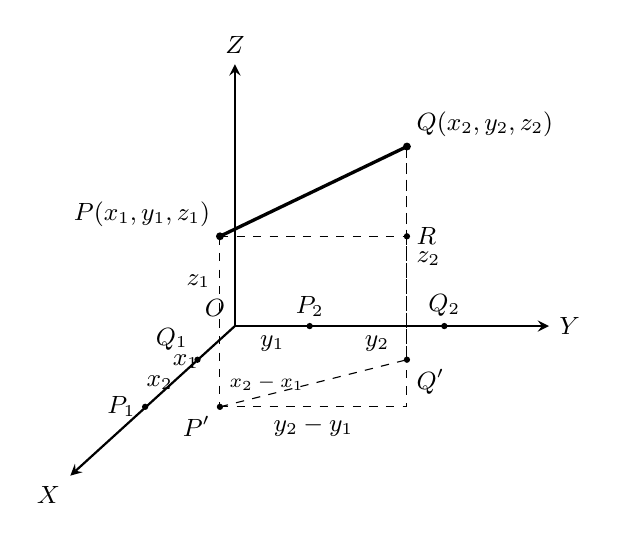
\begin{tikzpicture}[>=stealth, scale=0.95, font=\small]
  % Axes
  \draw[->, thick] (0, 0) -- (-2.2, -2.0) node[below left] {$X$};
  \draw[->, thick] (0, 0) -- (4.2, 0) node[right] {$Y$};
  \draw[->, thick] (0, 0) -- (0, 3.5) node[above] {$Z$};
  \node[above left] at (0, 0) {$O$};

  % Points P and Q
  % P coords: x1, y1, z1
  % Q coords: x2, y2, z2
  \coordinate (P1) at (-1.2, -1.08); % on X
  \coordinate (P2) at (1.0, 0);     % on Y
  \coordinate (Pprime) at (-0.2, -1.08); % proj of P on XY
  \coordinate (P) at (-0.2, 1.2);    % P

  \coordinate (Q1) at (-0.5, -0.45); % on X
  \coordinate (Q2) at (2.8, 0);      % on Y
  \coordinate (Qprime) at (2.3, -0.45); % proj of Q on XY
  \coordinate (Q) at (2.3, 2.4);     % Q

  % Box for PQ
  \coordinate (R) at (2.3, 1.2); % horizontal from P, vertical beneath Q
  \coordinate (S) at (2.3, -1.08); % in XY plane: same x as P, same y as Q

  \draw[very thick] (P) -- (Q);
  \draw[dashed] (P) -- (R) -- (Q);
  \draw[dashed] (P) -- (Pprime);
  \draw[dashed] (Q) -- (Qprime);
  \draw[dashed] (Pprime) -- (Qprime);
  \draw[dashed] (Pprime) -- (S) -- (Qprime);
  \draw[dashed] (R) -- (Qprime);

  \fill (P) circle (1.5pt) node[above left] {$P(x_1, y_1, z_1)$};
  \fill (Q) circle (1.5pt) node[above right] {$Q(x_2, y_2, z_2)$};
  \fill (R) circle (1.2pt) node[right] {$R$};
  \fill (Pprime) circle (1.2pt) node[below left] {$P'$};
  \fill (Qprime) circle (1.2pt) node[below right] {$Q'$};
  \fill (P1) circle (1.2pt) node[left] {$P_1$};
  \fill (Q1) circle (1.2pt) node[above left] {$Q_1$};
  \fill (P2) circle (1.2pt) node[above] {$P_2$};
  \fill (Q2) circle (1.2pt) node[above] {$Q_2$};

  \node[left] at (-0.2, 0.6) {$z_1$};
  \node[right] at (2.3, 0.9) {$z_2$};
  \node[below] at (1.05, -1.08) {$y_2 - y_1$};
  \node[below left] at (-0.7, -0.54) {$x_2$};
  \node[below] at (0.5, 0) {$y_1$};
  \node[below] at (1.9, 0) {$y_2$};
  \node[below left] at (-0.35, -0.25) {$x_1$};
  \node[left] at (1.05, -0.76) {\scriptsize $x_2 - x_1$};
\end{tikzpicture}
\caption{空間中兩點之距離分解}
\label{fig:b3-fig3-4}
\end{figure}

\begin{align*}
\overline{PQ}^2 &= \overline{PR}^2 + \overline{RQ}^2 = \overline{P'Q'}^2 + \overline{RQ}^2 = \overline{P'S}^2 + \overline{SQ'}^2 + \overline{RQ}^2 \\
&= |x_2 - x_1|^2 + |y_2 - y_1|^2 + |z_2 - z_1|^2 \\
&= (x_2 - x_1)^2 + (y_2 - y_1)^2 + (z_2 - z_1)^2
\end{align*}
故有
\begin{align*}
\overline{PQ} &= \sqrt{|x_2 - x_1|^2 + |y_2 - y_1|^2 + |z_2 - z_1|^2} \\
&= \sqrt{(x_2 - x_1)^2 + (y_2 - y_1)^2 + (z_2 - z_1)^2}.
\end{align*}

% =========================================================================
% § 3-2 從各種觀點看向量
% =========================================================================
\subsection{從各種觀點看向量}
\label{sec:b3-3-2}

\subsubsection*{甲、幾何觀點——相對位置的觀點}

第二章提過有向線段是「相對位置」的一種描寫. 嚴格說來，這樣的看法有一點漏洞：一個有向線段 $\vec{AB}$ 描寫的不止是 $B$ 點對 $A$ 點的「相對位置」. 比如 $B$ 在 $A$ 之東北方向 5 公里，有向線段 $\vec{AB}$ 不止說明「向東北走 5 公里」，它還特別指出是以 $A$ 為參考點的. 換句話說，有向線段 $\vec{AB}$ 的全義是「從 $A$ 點向東北走 5 公里」即達 $B$ 點，將這話拆解得三因素：「參考點（或稱始點）$A$」「東北方向」「5 公里」也就是說：一個有向線段是由下列三個因素組成：
\begin{center}
「始點」「方向」「距離（或長度）」
\end{center}

\begin{figure}[H]
\centering
\begin{tikzpicture}[>=stealth, scale=1.0, font=\small]
  \coordinate (A) at (0, 0);
  \coordinate (B) at (35:2.5);
  \draw[->, very thick] (A) -- (B) node[midway, above left] {5 公里};
  \fill (A) circle (1.5pt) node[below] {$A$};
  \fill (B) circle (1.5pt) node[right] {$B$};
\end{tikzpicture}
\caption{有向線段三要素}
\label{fig:b3-fig3-5}
\end{figure}

仔細分析：當我們說「相對位置」時，我們並不包含「始點」. 亦即，上例中我們提到「相對位置」時，指的是「向東北走 5 公里」而不管始點何處，換句話說「相對位置」是由
\begin{center}
「方向」與「距離（或長度）」
\end{center}
這兩個因素組成.

從幾何觀點，一個向量便是一個像上例「向東北走 5 公里」這樣的一個「相對位置」. 它不計始點但可以由一個有向線段來代表. 例如「向東北走 5 公里」這一向量 $\mathbf{a}$ 可以上圖有向線段 $\vec{AB}$ 來代表. 但兩個有向線段 $\vec{AB}, \vec{CD}$ 只要是同向且等長它們便有著同樣的方向與距離，\phantomsection\label{note:b3-ch3-p76-fig-ref}%
例如圖 3-6\footnote{【校訂註】原書此處印作「例如圖 3-7」，下文及次頁對應之兩向量同向等長插圖標記為「圖 3-6」（頁 76 原印圖 3-5 為單向量，圖 3-7 實為空間座標長度圖）。正文照原書字樣錄入並在此校記。}，$\vec{AB}, \vec{CD}$ 起點雖然不同，但它們都同樣朝東北方，都同樣走 5 公里，因此它們是代表同一向量的.

反過來，任兩有向線段 $\vec{AB}, \vec{CD}$ 若代表同一向量，依向量定義，$\vec{AB}$ 與 $\vec{CD}$ 有同樣方向，同樣長度，意即，$\vec{AB}$ 與 $\vec{CD}$ 同向且等長.

整理一下：向量是「相對位置」的一種描寫，它由「方向」與「距離」兩個因素構成. 任給一向量 $\mathbf{a}$，可以取一有向線段 $\vec{AB}$ 來代表 $\mathbf{a}$（亦即 $\mathbf{a}$ 與 $\vec{AB}$ 有同樣的方向與長度），但不同的有向線段可以代表同一個向量，其充要條件為：
\begin{align*}
\vec{AB} \text{ 與 } \vec{CD} \text{ 代表同一向量 } \mathbf{a} &\iff \vec{AB} \text{ 與 } \vec{CD} \text{ 同向且等長}.
\end{align*}

\begin{figure}[H]
\centering
\begin{tikzpicture}[>=stealth, scale=0.9, font=\small]
  \coordinate (A) at (0, 0);
  \coordinate (B) at (35:2.2);
  \coordinate (C) at (1.2, -0.6);
  \coordinate (D) at ($(C) + (35:2.2)$);

  \draw[->, very thick] (A) -- (B) node[midway, above left] {5 公里};
  \draw[->, very thick] (C) -- (D) node[midway, above left] {5 公里};

  \fill (A) circle (1.5pt) node[left] {$A$};
  \fill (B) circle (1.5pt) node[right] {$B$};
  \fill (C) circle (1.5pt) node[left] {$C$};
  \fill (D) circle (1.5pt) node[right] {$D$};
\end{tikzpicture}
\caption{同向且等長之有向線段代表同一向量}
\label{fig:b3-fig3-6}
\end{figure}

我們不妨用 $\mathbf{a} = \vec{AB}$ 來記述「有向線段 $\vec{AB}$ 代表向量 $\mathbf{a}$」這一現象，用等號 ``$=$'' 只是約定罷了. 我們又用 $\vec{AB} \sim \vec{CD}$ 來記述「$\vec{AB}$ 與 $\vec{CD}$ 同向且等長」.

注意一件事：給定一向量 $\mathbf{a}$，過任意一點 $A$，可唯一地引出一有向線段 $\vec{AB}$，使得
\[ \mathbf{a} = \vec{AB}. \]

\subsubsection*{乙、向量、點與座標}

我們已講過向量幾何是要把空間所有的點與向量的全體作一自然的一一對應. 上述的論析告訴我們：既然一個向量可由隨意取定其始點的同向等長線段來代表，我們不妨取一固定點 $O$ 當所有向量的始點，那麼向量的全體便與以 $O$ 為始點的有向線段的全體一一對應. 而給了一個空間的點 $A$，便對應一有向線段 $\vec{OA}$，這又是一個空間點的全體與以 $O$ 為始點的有向線段的全體間的一個一一對應.

因此藉著空間中一個任給的點，可把空間點的全體與向量的全體自然地一一對應起來. 這對應便是把幾何形象轉化成代數形式的原始基礎，向量代數便是在這些轉化生成的幾何量，即向量上面施以各種運算.

另一方面，在向量運算中可以進一步藉空間取定的座標系為準，以其對應點的座標來表示. 設所取的直角座標系為 $(O; X, Y, Z)$，向量 $\mathbf{a}$ 可以唯一地用一個有向線段 $\vec{OA}$ 代表. 因此可唯一地用點 $A$ 來代表，而點 $A$ 又可表為座標 $(x, y, z)$. 故向量 $\mathbf{a}$ 在此直角座標系 $(O; X, Y, Z)$ 中就可以用 $(x, y, z)$ 來代表. 稱 $(x, y, z)$ 為向量 $\mathbf{a}$ 相關於 $(O; X, Y, Z)$ 的座標表示，常記成
\[ \mathbf{a} = \vec{OA} = (x, y, z), \]
其中 $x, y, z$ 稱為向量 $\mathbf{a}$ 相關於 $(O; X, Y, Z)$ 的三個成分：$X$-成分，$Y$-成分，$Z$-成分，或簡稱為 $\mathbf{a}$ 的三個成分.

向量 $\mathbf{a}$ 的長度便是代表它的任一有向線段的長度. 若將 $\mathbf{a}$ 的長度記為 $|\mathbf{a}|$，則 $\mathbf{a} = \vec{OA} = (x, y, z)$ 時，
\[ |\mathbf{a}| = OA = \sqrt{x^2 + y^2 + z^2}. \]

\begin{figure}[H]
\centering
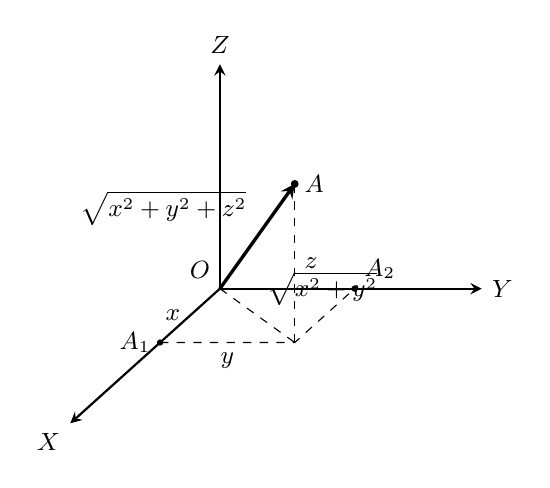
\begin{tikzpicture}[>=stealth, scale=0.95, font=\small]
  \draw[->, thick] (0, 0) -- (-2, -1.8) node[below left] {$X$};
  \draw[->, thick] (0, 0) -- (3.5, 0) node[right] {$Y$};
  \draw[->, thick] (0, 0) -- (0, 3) node[above] {$Z$};
  \node[above left] at (0, 0) {$O$};

  \coordinate (A1) at (-0.8, -0.72);
  \coordinate (A2) at (1.8, 0);
  \coordinate (Aprime) at (1.0, -0.72);
  \coordinate (A) at (1.0, 1.4);

  \draw[dashed] (A1) -- (Aprime) node[midway, below] {$y$} -- (A2);
  \draw[dashed] (0, 0) -- (Aprime) node[midway, above right] {$\sqrt{x^2+y^2}$};
  \draw[dashed] (Aprime) -- (A) node[midway, right] {$z$};
  \draw[very thick, ->] (0, 0) -- (A) node[midway, above left] {$\sqrt{x^2+y^2+z^2}$};

  \fill (A) circle (1.5pt) node[right] {$A$};
  \fill (A1) circle (1.2pt) node[left] {$A_1$};
  \fill (A2) circle (1.2pt) node[above right] {$A_2$};
  \node[left] at (-0.4, -0.36) {$x$};
\end{tikzpicture}
\caption{向量之長度}
\label{fig:b3-fig3-7}
\end{figure}

\begin{example}[論例 1]
回想一個平行四邊形的基本原理：若四邊形 $ABDC$ 在一平面上，則
\[ \vec{AB} \text{ 與 } \vec{CD} \text{ 同向且等長} \iff AB = CD, AC = BD. \]

利用這原理，我們來看如何在實際的座標空間中判斷兩個已知端點的有向線段代表同一向量.

設有平面上的四點 $A(-3, 2), B(2, 5), C(-1, -2), D(4, 1)$ 試證 $\vec{AB} \sim \vec{CD}$，並求其所共同代表的向量的座標.
\end{example}

\begin{proof}
(i) \phantomsection\label{note:b3-ch3-p78-fig3-9}%
由右圖 3-8\footnote{【校訂註】原書頁 78 末行及頁 79 倒數第 4 行兩度指涉「圖 3-9」，實指對應之描點插圖「圖 3-8」（頁 80 另有圖 3-9 說明移動觀點）。正文保留原書字樣並在此校記。}，知 $A, B, D, C$ 構成一平面上的四邊形，欲證明 $\vec{AB}$ 與 $\vec{CD}$ 同向且等長，即須證明
\[ AB = CD, \quad AC = BD \]
今
\begin{align*}
AB &= \sqrt{(2 - (-3))^2 + (5 - 2)^2} = \sqrt{34} \\
CD &= \sqrt{(4 - (-1))^2 + (1 - (-2))^2} = \sqrt{34} \\
AC &= \sqrt{((-1) - (-3))^2 + ((-2) - 2)^2} = \sqrt{20} \\
BD &= \sqrt{(4 - 2)^2 + (1 - 5)^2} = \sqrt{20}
\end{align*}
故 $AB = CD, AC = BD$，得證 $\vec{AB} \sim \vec{CD}$.

\begin{figure}[H]
\centering
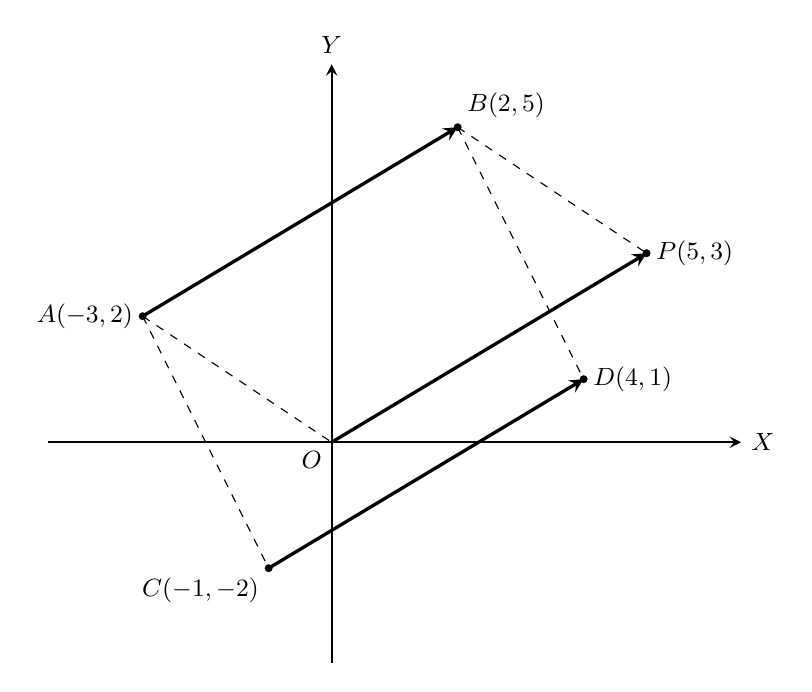
\begin{tikzpicture}[>=stealth, scale=0.8, font=\small]
  \draw[->, thick] (-4.5, 0) -- (6.5, 0) node[right] {$X$};
  \draw[->, thick] (0, -3.5) -- (0, 6) node[above] {$Y$};
  \node[below left] at (0, 0) {$O$};

  \coordinate (A) at (-3, 2);
  \coordinate (B) at (2, 5);
  \coordinate (C) at (-1, -2);
  \coordinate (D) at (4, 1);
  \coordinate (P) at (5, 3);

  \draw[very thick, ->] (A) -- (B);
  \draw[very thick, ->] (C) -- (D);
  \draw[very thick, ->] (0, 0) -- (P);

  \draw[dashed] (A) -- (C);
  \draw[dashed] (B) -- (D);
  \draw[dashed] (B) -- (P);
  \draw[dashed] (A) -- (0, 0);

  \fill (A) circle (1.8pt) node[left] {$A(-3, 2)$};
  \fill (B) circle (1.8pt) node[above right] {$B(2, 5)$};
  \fill (C) circle (1.8pt) node[below left] {$C(-1, -2)$};
  \fill (D) circle (1.8pt) node[right] {$D(4, 1)$};
  \fill (P) circle (1.8pt) node[right] {$P(5, 3)$};
\end{tikzpicture}
\caption{平面點與向量同向等長驗證}
\label{fig:b3-fig3-8}
\end{figure}

(ii) $\vec{AB}$ 既然與 $\vec{CD}$ 同向且等長，則決定同一向量，設為 $\mathbf{a}$，欲求向量 $\mathbf{a}$ 的座標表示，即欲求點 $P(x, y)$ 使得 $\mathbf{a} = \vec{OP}$，如此而得 $\mathbf{a} = (x, y)$. 為此我們做這樣的猜想：

$\vec{AB}$ 可看成是從始點 $A$ 沿 $OX$ 方向移動 $2 - (-3) = 5$ 單位，次沿 $OY$ 方向移動 $5 - 2 = 3$ 單位才到達 $B$ 的，既然 $\vec{OP}$ 要與 $\vec{AB}$ 代表同一向量 $\mathbf{a}$，它們除了起點不同外，移動的方式``該是''一樣的. 從原點 $O$ 沿 $OX$ 移動 5 單位，再沿 $OY$ 移動 3 單位，到達的位置取為 $P$，則 $P$ 點的座標為 $(5, 3)$.

我們要用上述基本原理來驗證 $\vec{AB} \sim \vec{OP}$，根據描點於圖 3-8 上，知 $ABPO$ 為一平面上的四邊形.
今
\begin{align*}
OP &= \sqrt{5^2 + 3^2} = \sqrt{34} = AB \\
OA &= \sqrt{3^2 + 2^2} = \sqrt{13} \\
PB &= \sqrt{(2 - 5)^2 + (5 - 3)^2} = \sqrt{13}
\end{align*}
故 $OP = AB, OA = PB$，得證 $\vec{OP} \sim \vec{AB}$.
因此
\[ \mathbf{a} = \vec{OP} = \vec{AB} = (5, 3). \qedhere \]
\end{proof}

\subsubsection*{作業 1}
在平面上，有兩點 $A(1, -2), B(2, -4)$，試求有向線段 $\vec{AB}$ 所代表的向量的座標表示，須加以驗證.

\subsubsection*{丙、移動觀點}

一個向量其實可以看成一個空間所有點的同向而等長的移動（簡稱平移），〔平行而等長的移動意思是：設 $A, C$ 為空間中任兩點，移動後搬到 $B, D$ 的位置 $\vec{AB}$ 與 $\vec{CD}$ 同向且等長.〕

像甲段中反覆舉為例子的一個向量，「向東北走 5 公里」顯然可以看成空間中所有點向東北走 5 公里的移動.

這樣的觀點使下節將要定義向量和有了很自然的意義：

設 $\mathbf{a}$ 表「向東北移 5 公里」的向量，$\mathbf{b}$ 表「向東南移 5 公里」的向量. 則 $\mathbf{a} + \mathbf{b}$ 要代表兩個移動的連續實施，將所有點先向東北移 5 公里，再向東南移 5 公里，結果是「向東移 $5\sqrt{2}$ 公里」. 亦即：$\mathbf{a} + \mathbf{b}$ 代表「向東移 $5\sqrt{2}$ 公里」這一向量.

向量加法的嚴密定義，為下節的主題，這裏提起它，只是要闡明移動觀點在向量加法上有自然的解釋.

\begin{figure}[H]
\centering
\begin{minipage}{0.48\textwidth}
\centering
\begin{tikzpicture}[>=stealth, scale=0.9, font=\small]
  \coordinate (A) at (0, 0);
  \coordinate (B) at (30:2.2);
  \coordinate (C) at (0, -1);
  \coordinate (D) at ($(C) + (30:2.2)$);

  \draw[->, very thick] (A) -- (B);
  \draw[->, very thick] (C) -- (D);

  \fill (A) circle (1.2pt) node[left] {$A$};
  \fill (B) circle (1.2pt) node[right] {$B$};
  \fill (C) circle (1.2pt) node[left] {$C$};
  \fill (D) circle (1.2pt) node[right] {$D$};
\end{tikzpicture}
\caption{空間點同向等長移動}
\label{fig:b3-fig3-9}
\end{minipage}
\hfill
\begin{minipage}{0.48\textwidth}
\centering
\begin{tikzpicture}[>=stealth, scale=0.85, font=\small]
  \coordinate (O) at (0, 0);
  \coordinate (A) at (45:2.5);
  \coordinate (B) at (3.535, 0);

  \draw[->, very thick] (O) -- (A) node[midway, above left] {5公里};
  \draw[->, very thick] (A) -- (B) node[midway, above right] {5公里};
  \draw[->, very thick] (O) -- (B) node[midway, below] {$5\sqrt{2}$ 公里};
\end{tikzpicture}
\caption{兩連續移動的合成}
\label{fig:b3-fig3-10}
\end{minipage}
\end{figure}

\subsubsection*{丁、力學觀點}

在力學上我們慣於用有向線段來代表一些物理量，如力、速度、加速度等.

力有三要素：「施力點」、「施力方向」、「施力大小」，這些相當於幾何觀點中有向線段之「始點」、「方向」、「長度」. 也因此，我們用有向線段來圖解力. 如：

\begin{figure}[H]
\centering
\begin{minipage}{0.48\textwidth}
\centering
\begin{tikzpicture}[>=stealth, scale=0.9, font=\small]
  \coordinate (A) at (0, 2);
  \coordinate (B) at (1, 0.2);
  \draw[->, very thick] (A) -- (B) node[midway, right] {300 公斤};
  \fill (A) circle (1.5pt) node[left] {$A$};
  \fill (B) circle (1.5pt) node[below] {$B$};

  \coordinate (C) at (3, 1.8);
  \coordinate (D) at (3, 0.6);
  \draw[->, very thick] (C) -- (D) node[midway, right] {100 公斤};
  \fill (C) circle (1.5pt) node[above] {$C$};
  \fill (D) circle (1.5pt) node[below] {$D$};
\end{tikzpicture}
\caption{力的作用點、方向與大小}
\label{fig:b3-fig3-11}
\end{minipage}
\hfill
\begin{minipage}{0.48\textwidth}
\centering
\begin{tikzpicture}[>=stealth, scale=0.9, font=\small]
  \coordinate (O) at (0, 0);
  \coordinate (A) at (1.8, 0);
  \coordinate (B) at (0.8, 1.2);
  \coordinate (C) at ($(A) + (B)$);

  \draw[->, very thick] (O) -- (A) node[midway, below] {$\mathbf{a}$};
  \draw[->, very thick] (O) -- (B) node[midway, above left] {$\mathbf{b}$};
  \draw[dashed] (B) -- (C);
  \draw[dashed] (A) -- (C);
  \draw[->, very thick] (O) -- (C) node[midway, above left] {$\mathbf{a}+\mathbf{b}$};

  \node[right] at (2.6, 0.5) {$\mathbf{a}$ 與 $\mathbf{b}$ 的合成立};
\end{tikzpicture}
\caption{力的合成平行四邊形}
\label{fig:b3-fig3-12}
\end{minipage}
\end{figure}

作用點分別是 $A, C$. 施力方向則分別沿 $\vec{AB}, \vec{CD}$，而力的大小按比例由 $\overline{AB}$ 與 $\overline{CD}$ 之長度給定，如上圖 $\vec{AB}$ 與 $\vec{CD}$ 的大小分別為 300 公斤、100 公斤，相應線段長度之比為 $3 : 1$.

在實際力學問題的處理中常常不需力的施力點，我們所注意到的只是力的方向與大小，這時我們就把力看成一個向量，以便於計算.

向量的加法用力學觀點也有它實際的意義. 兩個力作為向量依向量加法取得之和，恰巧就是合成立.

\subsubsection*{習題 3-2}

\begin{enumerate}[label=\arabic*., leftmargin=2em]
  \item 試證平移把一直線移成另一平行的直線.〔取 $L$ 上一點 $A$，設 $A$ 經平移後到 $A'$，過 $A'$ 作一平行於 $L$ 的直線 $L'$. 證明 $L$ 上任一點 $P$ 經平移後皆落在 $L'$ 上，反過來 $L'$ 上的點皆自 $L$ 上的點平移過來〕
  \item 證證平移保持長度不變，亦即空間中 $A, B$ 兩點經一向量 $\mathbf{a}$ 所對應的平移後搬到 $A', B'$ 兩點位置，則 $\overline{AB} = \overline{A'B'}$.\\
  （注意：由上二題的結果可以看出：向量准許平移.）
  \item 試證平行四邊形經平移後，還是平行四邊形. 矩形經平移後還是矩形. 而正方形平移後呢？
  \item 圖示下列各向量：
  \[ \mathbf{a} = \text{向東三公分}, \quad \mathbf{b} = \text{向西北四公分}, \quad \mathbf{c} = \text{向東南二公分}. \]
  \item 甲行進速度每小時四公里，乙每小時三公里，二人自同一點出發，甲向東行進，乙向東北行進，三小時後二人的相對位置如何，試用向量表示.
  \item 對相關座標系 $(O; X, Y)$ 有向量 $\mathbf{a} = (s + t, 3s - t) = (4, -6)$；試求 $s$ 與 $t$. 又如果以 $P(3, 5)$ 為起點，即 $\mathbf{a} = \vec{PQ}$，則 $Q$ 座落在那裏？
  \item 如將一正方形先依一向量 $\mathbf{a}$ 平移，再依一向量 $\mathbf{b}$ 平移，試問可否將此正方形自後來位置經過一適當（？）向量的平移回到原來位置？試將此作用繪圖表示.
  \item 試繪圖表示一正立方體在空間平移的圖形.
\end{enumerate}

% =========================================================================
% § 3-3 向量的加減法
% =========================================================================
\subsection{向量的加減法}
\label{sec:b3-3-3}

\subsubsection*{甲、向量加法的幾何意義}

上節移動與力學的觀點已多少表明了向量和的用意. 現在我們回復用淺易的幾何觀點——有向線段來下它的定義：

任給兩向量 $\mathbf{a}$ 與 $\mathbf{b}$，取有向線段 $\vec{AB}$ 與 $\vec{BC}$ 使
\[ \mathbf{a} = \vec{AB}, \quad \mathbf{b} = \vec{BC} \]
先定義這種首尾相接的有向線段的和 $\vec{AB} + \vec{BC}$ 為
\[ \vec{AB} + \vec{BC} = \vec{AC} \]
這是很自然的定義，從 $A$ 沿 $\vec{AB}$ 到 $B$ 再沿 $\vec{BC}$ 到 $C$，結果相當於直接從 $A$ 到 $C$.

\begin{figure}[H]
\centering
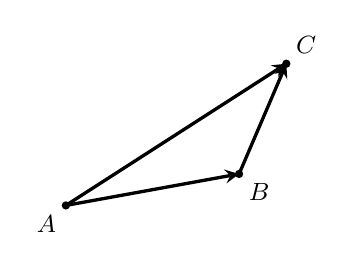
\begin{tikzpicture}[>=stealth, scale=1.0, font=\small]
  \coordinate (A) at (0, 0);
  \coordinate (B) at (2.2, 0.4);
  \coordinate (C) at (2.8, 1.8);

  \draw[->, very thick] (A) -- (B) node[midway, below] {};
  \draw[->, very thick] (B) -- (C) node[midway, right] {};
  \draw[->, very thick] (A) -- (C) node[midway, above left] {};

  \fill (A) circle (1.5pt) node[below left] {$A$};
  \fill (B) circle (1.5pt) node[below right] {$B$};
  \fill (C) circle (1.5pt) node[above right] {$C$};
\end{tikzpicture}
\caption{首尾相接有向線段之和}
\label{fig:b3-fig3-13}
\end{figure}

但如果拿 $\vec{AC}$ 所代表的向量 $\mathbf{c}$（亦即 $\mathbf{c} = \vec{AC}$）作為向量和 $\mathbf{a} + \mathbf{b}$，會不會有毛病？

換句話說，如果重新開始我們取的是 $\vec{A'B'}$ 與 $\vec{B'C'}$，使
\[ \mathbf{a} = \vec{A'B'}, \quad \mathbf{b} = \vec{B'C'} \]
則 $\vec{A'C'}$ 是否正好與 $\vec{AC}$ 代表同一向量 $\mathbf{c}$？亦即 $\vec{A'C'}$ 與 $\vec{AC}$ 是否同向且等長？即，是否
\[ \vec{A'B'} \sim \vec{AB}, \ \vec{B'C'} \sim \vec{BC} \implies \vec{A'C'} \sim \vec{AC}? \]

\phantomsection\label{note:b3-ch3-p83-sec-ref}%
答案是肯定的. 由 §3-1\footnote{【校訂註】原書作「由 §3-1 提過的平行四邊形的基本原理知」，該平行四邊形原理實敘述於 § 3-2 乙（頁 78【論例 1】）。正文照原書字樣錄入。} 提過的平行四邊形的基本原理知
\begin{align*}
\vec{AA'} &\sim \vec{BB'}, \\
\vec{BB'} &\sim \vec{CC'}
\end{align*}
故 $\vec{AA'} \sim \vec{CC'}$. 因此 $\square AA'C'C$ 為一平行四邊形，故
\[ \vec{A'C'} \sim \vec{AC}. \quad \# \]

\begin{figure}[H]
\centering
\begin{tikzpicture}[>=stealth, scale=0.9, font=\small]
  \coordinate (A) at (0, 0);
  \coordinate (B) at (2.2, 0.2);
  \coordinate (C) at (3.0, 1.4);

  \coordinate (Aprime) at (-1.2, 1.6);
  \coordinate (Bprime) at ($(B) + (-1.2, 1.6)$);
  \coordinate (Cprime) at ($(C) + (-1.2, 1.6)$);

  \draw[->, thick] (A) -- (B);
  \draw[->, thick] (B) -- (C);
  \draw[->, very thick] (A) -- (C);

  \draw[->, thick] (Aprime) -- (Bprime);
  \draw[->, thick] (Bprime) -- (Cprime);
  \draw[->, very thick] (Aprime) -- (Cprime);

  \draw[dashed] (A) -- (Aprime);
  \draw[dashed] (B) -- (Bprime);
  \draw[dashed] (C) -- (Cprime);

  \fill (A) circle (1.5pt) node[below] {$A$};
  \fill (B) circle (1.5pt) node[below right] {$B$};
  \fill (C) circle (1.5pt) node[right] {$C$};
  \fill (Aprime) circle (1.5pt) node[left] {$A'$};
  \fill (Bprime) circle (1.5pt) node[above left] {$B'$};
  \fill (Cprime) circle (1.5pt) node[above right] {$C'$};
\end{tikzpicture}
\caption{向量和的客觀一致性}
\label{fig:b3-fig3-14}
\end{figure}

這樣，我們定義向量和如下：
\begin{definition}
任給兩向量 $\mathbf{a}$ 與 $\mathbf{b}$，取首尾相接的有向線段 $\vec{AB}$ 與 $\vec{BC}$ 分別表 $\mathbf{a}$ 與 $\mathbf{b}$，則定義
\[ \mathbf{c} = \vec{AB} + \vec{BC} = \vec{AC} \]
為向量和 $\mathbf{a} + \mathbf{b}$，亦即
\[ \mathbf{a} + \mathbf{b} = \vec{AC}. \]
\end{definition}

再用移動的觀點來看，這定義前的解釋，正好說明了下一事實：「兩個向量 $\mathbf{a}, \mathbf{b}$ 相應的平移的連續實施，也是一個平移（即 $\vec{A'B'} \sim \vec{AB}, \vec{B'C'} \sim \vec{BC} \implies \vec{A'C'} \sim \vec{AC}$），而所得的平移便相應於向量和 $\mathbf{a} + \mathbf{b}$.」

\begin{figure}[H]
\centering
\begin{minipage}{0.48\textwidth}
\centering
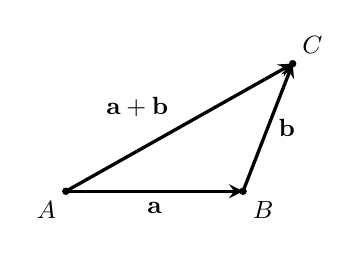
\begin{tikzpicture}[>=stealth, scale=0.9, font=\small]
  \coordinate (A) at (0, 0);
  \coordinate (B) at (2.5, 0);
  \coordinate (C) at (3.2, 1.8);

  \draw[->, very thick] (A) -- (B) node[midway, below] {$\mathbf{a}$};
  \draw[->, very thick] (B) -- (C) node[midway, right] {$\mathbf{b}$};
  \draw[->, very thick] (A) -- (C) node[midway, above left] {$\mathbf{a}+\mathbf{b}$};

  \fill (A) circle (1.5pt) node[below left] {$A$};
  \fill (B) circle (1.5pt) node[below right] {$B$};
  \fill (C) circle (1.5pt) node[above right] {$C$};
\end{tikzpicture}
\caption{向量加法三角形法則}
\label{fig:b3-fig3-15}
\end{minipage}
\hfill
\begin{minipage}{0.48\textwidth}
\centering
\begin{tikzpicture}[>=stealth, scale=0.9, font=\small]
  \coordinate (O) at (0, 0);
  \coordinate (A) at (2.5, 0.4);
  \coordinate (B) at (0.2, 1.8);
  \coordinate (C) at ($(A) + (B)$);

  \draw[->, very thick] (O) -- (A) node[midway, below] {$\mathbf{a}$};
  \draw[->, very thick] (O) -- (B) node[midway, left] {$\mathbf{b}$};
  \draw[->, thick] (A) -- (C) node[midway, right] {$\mathbf{b}$};
  \draw[->, thick] (B) -- (C);
  \draw[->, very thick] (O) -- (C) node[midway, above left] {$\mathbf{a}+\mathbf{b}$};

  \fill (O) circle (1.5pt) node[below left] {$O$};
  \fill (A) circle (1.5pt) node[below right] {$A$};
  \fill (B) circle (1.5pt) node[above left] {$B$};
  \fill (C) circle (1.5pt) node[above right] {$C$};
\end{tikzpicture}
\caption{向量加法平行四邊形法則}
\label{fig:b3-fig3-16}
\end{minipage}
\end{figure}

上節乙段強調過對每一向量，取一通過原點 $O$ 的有向線段作為代表，如此則向量的全體一一對應於通過原點 $O$ 的有向線段的全體. 這樣的觀點或力學合成力的觀點都要求我們考慮如下的問題：

設「$\mathbf{a} = \vec{OA}, \mathbf{b} = \vec{OB}$，則 $\mathbf{a} + \mathbf{b} = ?$」

作 $C$ 點使四邊形 $OACB$ 做成一個平行四邊形，連結 $OC$，則因
\[ \vec{AC} \sim \vec{OB} \quad \text{故 } \mathbf{b} = \vec{AC} \]
根據上述向量和定義，既然 $\mathbf{a} = \vec{OA}, \mathbf{b} = \vec{AC}$ 且 $\vec{OA}, \vec{AC}$ 首尾相接，則
\[ \mathbf{a} + \mathbf{b} = \vec{OC}. \quad \# \]

\subsubsection*{乙、向量加法的基本性質}

在第一冊討論數的運算時，我們知道數的加法，具有交換律、結合律、可逆性等有用的優良通性. 向量的加法也具有這一類性質.

\begin{enumerate}[label=(\Roman*), leftmargin=2em]
  \item \textbf{結合律}\quad 設 $\mathbf{a}, \mathbf{b}, \mathbf{c}$ 為空間中任給之向量，取 $A, B, C, D$ 四點，使得
  \[ \mathbf{a} = \vec{AB}, \quad \mathbf{b} = \vec{BC}, \quad \mathbf{c} = \vec{CD}. \]
  故 $\mathbf{a} + \mathbf{b} = \vec{AC}$，故 $(\mathbf{a} + \mathbf{b}) + \mathbf{c} = \vec{AD}$.
  另一方面
  \[ \mathbf{b} + \mathbf{c} = \vec{BD}, \quad \text{故 } \mathbf{a} + (\mathbf{b} + \mathbf{c}) = \vec{AD} \]
  因此向量加法滿足結合律：
  \[ (\mathbf{a} + \mathbf{b}) + \mathbf{c} = \mathbf{a} + (\mathbf{b} + \mathbf{c}). \]

\begin{figure}[H]
\centering
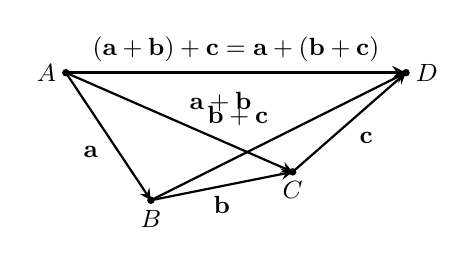
\begin{tikzpicture}[>=stealth, scale=0.9, font=\small]
  \coordinate (A) at (0, 1.8);
  \coordinate (B) at (1.2, 0);
  \coordinate (C) at (3.2, 0.4);
  \coordinate (D) at (4.8, 1.8);

  \draw[->, thick] (A) -- (B) node[midway, below left] {$\mathbf{a}$};
  \draw[->, thick] (B) -- (C) node[midway, below] {$\mathbf{b}$};
  \draw[->, thick] (C) -- (D) node[midway, below right] {$\mathbf{c}$};

  \draw[->, thick] (A) -- (C) node[midway, above right] {$\mathbf{a}+\mathbf{b}$};
  \draw[->, thick] (B) -- (D) node[midway, above left] {$\mathbf{b}+\mathbf{c}$};
  \draw[->, very thick] (A) -- (D) node[midway, above] {$(\mathbf{a}+\mathbf{b})+\mathbf{c} = \mathbf{a}+(\mathbf{b}+\mathbf{c})$};

  \fill (A) circle (1.5pt) node[left] {$A$};
  \fill (B) circle (1.5pt) node[below] {$B$};
  \fill (C) circle (1.5pt) node[below] {$C$};
  \fill (D) circle (1.5pt) node[right] {$D$};
\end{tikzpicture}
\caption{向量加法結合律}
\label{fig:b3-fig3-17}
\end{figure}

  \item \textbf{交換律}\quad 設 $\mathbf{a}, \mathbf{b}$ 為空間中任給兩向量，取 $A, B, C$，使 $\mathbf{a} = \vec{AB}, \mathbf{b} = \vec{BC}$，則 $\mathbf{a} + \mathbf{b} = \vec{AC}$.\\
  另一方面作平行四邊形 $ABCD$，則
  \[ \vec{AD} \sim \vec{BC}, \quad \vec{DC} \sim \vec{AB} \]
  故 $\mathbf{b} = \vec{AD}, \mathbf{a} = \vec{DC}$.
  因此由向量和定義
  \[ \mathbf{b} + \mathbf{a} = \vec{AC} \]
  故
  \[ \mathbf{a} + \mathbf{b} = \mathbf{b} + \mathbf{a}. \]

\begin{figure}[H]
\centering
\begin{tikzpicture}[>=stealth, scale=0.9, font=\small]
  \coordinate (A) at (0, 0);
  \coordinate (B) at (3.5, 0.2);
  \coordinate (D) at (0.3, 1.8);
  \coordinate (C) at ($(B) + (D)$);

  \draw[->, very thick] (A) -- (B) node[midway, below] {$\mathbf{a}$};
  \draw[->, thick] (B) -- (C) node[midway, right] {$\mathbf{b}$};
  \draw[->, very thick] (A) -- (D) node[midway, left] {$\mathbf{b}$};
  \draw[->, thick] (D) -- (C) node[midway, above] {$\mathbf{a}$};
  \draw[->, very thick] (A) -- (C) node[midway, above left, sloped] {$(\mathbf{a}+\mathbf{b}) = (\mathbf{b}+\mathbf{a})$};

  \fill (A) circle (1.5pt) node[below left] {$A$};
  \fill (B) circle (1.5pt) node[below right] {$B$};
  \fill (D) circle (1.5pt) node[above left] {$D$};
  \fill (C) circle (1.5pt) node[above right] {$C$};
\end{tikzpicture}
\caption{向量加法交換律}
\label{fig:b3-fig3-18}
\end{figure}

  \item \textbf{零向量及其特徵}\quad 取一長度為零的有向線段 $\vec{AA}$，它所代表的向量，稱為零向量，記以 $\mathbf{0}$，須注意此時 $\mathbf{0}$ 之方向可任意取.\\
  對任一向量 $\mathbf{a} = \vec{AB}$，因 $\mathbf{0} = \vec{AA} \sim \vec{BB}$，故
  \begin{align*}
  \mathbf{0} + \mathbf{a} &= \vec{AB} = \mathbf{a} \\
  \mathbf{a} + \mathbf{0} &= \vec{AB} = \mathbf{a}
  \end{align*}
  這個對於任意 $\mathbf{a}$，$\mathbf{0} + \mathbf{a} = \mathbf{a} = \mathbf{a} + \mathbf{0}$ 是零向量的特徵，零向量所相應的空間中的平移是一個``原地不動的移動''.

  \item \textbf{可逆性}\quad 對任意向量 $\mathbf{a} = \vec{AB}$，考慮有向線段 $\vec{BA}$ 所代表的向量，稱為 $\mathbf{a}$ 的逆向量，記為 $-\mathbf{a}$，它的特徵是
  \[ \mathbf{a} + (-\mathbf{a}) = \mathbf{0} = (-\mathbf{a}) + \mathbf{a} \]
  此因 $\mathbf{a} = \vec{AB}, (-\mathbf{a}) = \vec{BA}$，兩有向線段首尾相連故
  \[ \mathbf{a} + (-\mathbf{a}) = \vec{AA} = \mathbf{0} \]
  同樣 $(-\mathbf{a}) + \mathbf{a} = \mathbf{0}$. \qedhere
\end{enumerate}

整理一下：對於空間中任給向量 $\mathbf{a}, \mathbf{b}, \mathbf{c}$，向量加法滿足
\begin{itemize}[leftmargin=3em]
  \item[(I)] 結合律\quad $(\mathbf{a} + \mathbf{b}) + \mathbf{c} = \mathbf{a} + (\mathbf{b} + \mathbf{c})$.
  \item[(II)] 交換律\quad $\mathbf{a} + \mathbf{b} = \mathbf{b} + \mathbf{a}$.
  \item[(III)] 存在零向量 $\mathbf{0}$，使得 $\mathbf{a} + \mathbf{0} = \mathbf{a} = \mathbf{0} + \mathbf{a}$.
  \item[(IV)] 存在逆向量 $(-\mathbf{a})$，使得 $\mathbf{a} + (-\mathbf{a}) = \mathbf{0} = (-\mathbf{a}) + \mathbf{a}$.
\end{itemize}

\subsubsection*{丙、向量的分解與加法的座標成分表示}

我們要說明對於這樣一個富有幾何意義的向量加法，若用座標成分表示，其實很是原始而易於明瞭.

\phantomsection\label{note:b3-ch3-p87-fig-ref}%
先注意一件事，任給一向量 $\mathbf{a}$，表 $\mathbf{a} = \vec{OA}$，則 $\mathbf{a}$ 可分解成三個分別沿著 $X, Y, Z$ 軸的向量 $\mathbf{a}_x, \mathbf{a}_y, \mathbf{a}_z$，其中（如圖 3-19\footnote{【校訂註】原書此處行文印作「如圖 3-20」，下文插圖標記為「圖 3-19」。正文保留原書字樣並在此校記。}）
\begin{align*}
\mathbf{a}_x &= \vec{OA_1} \\
\mathbf{a}_y &= \vec{A_1 A'} \\
\mathbf{a}_z &= \vec{A'A}
\end{align*}
也就是說，$\mathbf{a} = \vec{OA} = \vec{OA_1} + \vec{A_1 A'} + \vec{A'A} = \mathbf{a}_x + \mathbf{a}_y + \mathbf{a}_z$，$\mathbf{a}_x, \mathbf{a}_y$ 與 $\mathbf{a}_z$ 分別稱為向量 $\mathbf{a}$ 在 $X$-軸、$Y$-軸與 $Z$-軸上的分向量，另一方面，設 $\mathbf{a} = (x, y, z)$，則知
\begin{center}
$\mathbf{a}_x$ 的長度為 $x$ 的絕對值；當 $x$ 為正，$\mathbf{a}_x$ 與 $\vec{OX}$ 同向，當 $x$ 為負，$\mathbf{a}_x$ 與 $\vec{OX}$ 異向（這事將在第四節有一個較好的解說）
\end{center}
同樣的情形也發生在 $\mathbf{a}_y$ 與 $y$ 之間，以及在 $\mathbf{a}_z$ 與 $z$ 之間.

\begin{figure}[H]
\centering
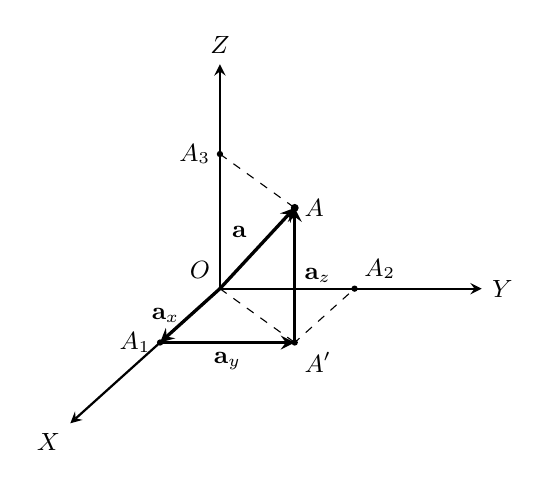
\begin{tikzpicture}[>=stealth, scale=0.95, font=\small]
  \draw[->, thick] (0, 0) -- (-2, -1.8) node[below left] {$X$};
  \draw[->, thick] (0, 0) -- (3.5, 0) node[right] {$Y$};
  \draw[->, thick] (0, 0) -- (0, 3) node[above] {$Z$};
  \node[above left] at (0, 0) {$O$};

  \coordinate (A1) at (-0.8, -0.72);
  \coordinate (A2) at (1.8, 0);
  \coordinate (A3) at (0, 1.8);
  \coordinate (Aprime) at (1.0, -0.72);
  \coordinate (A) at (1.0, 1.08);

  % Draw box
  \draw[dashed] (A1) -- (Aprime) node[midway, below] {$\mathbf{a}_y$} -- (A2);
  \draw[dashed] (Aprime) -- (A) node[midway, right] {$\mathbf{a}_z$};
  \draw[dashed] (0, 0) -- (Aprime);
  \draw[dashed] (A3) -- (A);

  % Vectors
  \draw[->, very thick] (0, 0) -- (A1) node[midway, left] {$\mathbf{a}_x$};
  \draw[->, very thick] (A1) -- (Aprime);
  \draw[->, very thick] (Aprime) -- (A);
  \draw[->, very thick] (0, 0) -- (A) node[midway, above left] {$\mathbf{a}$};

  \fill (A) circle (1.5pt) node[right] {$A$};
  \fill (A1) circle (1.2pt) node[left] {$A_1$};
  \fill (A2) circle (1.2pt) node[above right] {$A_2$};
  \fill (A3) circle (1.2pt) node[left] {$A_3$};
  \fill (Aprime) circle (1.2pt) node[below right] {$A'$};
\end{tikzpicture}
\caption{向量在三軸之分向量分解}
\label{fig:b3-fig3-19}
\end{figure}

這樣的觀點很有助於我們來剖析加法的座標成分表示.

很容易看出零向量的三個成分均為零，即
\[ \mathbf{0} = (0, 0, 0). \]

另一方面，若 $\mathbf{a} = \vec{OA} = (x, y, z)$，取 $A'(-x, -y, -z)$ 為 $A(x, y, z)$ 對於原點 $O$ 點的對稱點. 因 $A, O, A'$ 共線且 $\vec{AO} = \vec{OA'}$，故
\[ \vec{AO} \sim \vec{OA'} \]
因 $\mathbf{a}$ 的逆向量 $(-\mathbf{a}) = \vec{AO}$，故
\[ (-\mathbf{a}) = \vec{OA'} = (-x, -y, -z). \]

\begin{theorem}
設 $\mathbf{a} = (x_1, y_1, z_1), \mathbf{b} = (x_2, y_2, z_2)$，則
\[ \mathbf{a} + \mathbf{b} = (x_1 + x_2, y_1 + y_2, z_1 + z_2). \]
\end{theorem}

\begin{proof}[解說]
根據上面分析 $\mathbf{a} = \mathbf{a}_x + \mathbf{a}_y + \mathbf{a}_z, \mathbf{b} = \mathbf{b}_x + \mathbf{b}_y + \mathbf{b}_z$，那麼
\begin{align*}
\mathbf{a} + \mathbf{b} &= (\mathbf{a}_x + \mathbf{a}_y + \mathbf{a}_z) + (\mathbf{b}_x + \mathbf{b}_y + \mathbf{b}_z) \\
&= (\mathbf{a}_x + \mathbf{b}_x) + (\mathbf{a}_y + \mathbf{b}_y) + (\mathbf{a}_z + \mathbf{b}_z) \quad \text{〔結合律及交換律〕}
\end{align*}
也就是 $\mathbf{a} + \mathbf{b}$ 的向量便是由以下三步驟得來：
\begin{center}
先沿 $X$ 軸走 $\mathbf{a}_x + \mathbf{b}_x$\\
次沿 $Y$ 軸走 $\mathbf{a}_y + \mathbf{b}_y$\\
再沿 $Z$ 軸走 $\mathbf{a}_z + \mathbf{b}_z$
\end{center}
換句話說 $\mathbf{a} + \mathbf{b}$ 的向量便是由原點 $O$
\begin{align*}
&\text{先沿 } OX \text{ 方向走 } x_1 + x_2 \text{ 的路 } \left[\begin{array}{l} x_1, x_2 \text{ 或 } x_1 + x_2 < 0 \text{ 時表示}\\ \text{相應行進的方向應調頭回走} \end{array}\right] \\
&\text{次沿 } OY \text{ 方向走 } y_1 + y_2 \text{ 的路} \\
&\text{再沿 } OZ \text{ 方向走 } z_1 + z_2 \text{ 的路}
\end{align*}
故 $\mathbf{a} + \mathbf{b}$ 的三個座標成分其實就是 $x_1 + x_2, y_1 + y_2, z_1 + z_2$，亦即
\[ \mathbf{a} + \mathbf{b} = (x_1 + x_2, y_1 + y_2, z_1 + z_2). \qedhere \]
\end{proof}

\phantomsection\label{note:b3-ch3-p88-fig-ref}%
下圖 3-20-1, 圖 3-20-2\footnote{【校訂註】原書頁 88 倒數第 2 行印作「下圖 3-21-1, 圖 3-21-2」，次頁對應插圖標記為「圖 3-20-1」與「圖 3-20-2」。正文保留原書字樣並在此校記。} 顯示平面上兩向量 $\mathbf{a} = \vec{OA} = (x_1, y_1), \mathbf{b} = \vec{OB} = (x_2, y_2)$ 之和 $\mathbf{a} + \mathbf{b} = \vec{OC}$ 的座標成分表示為 $(x_1 + x_2, y_1 + y_2)$.

\begin{figure}[H]
\centering
\begin{minipage}{0.48\textwidth}
\centering
\begin{tikzpicture}[>=stealth, scale=0.85, font=\small]
  \draw[->, thick] (-0.5, 0) -- (4.2, 0) node[right] {$X$};
  \draw[->, thick] (0, -0.5) -- (0, 3.8) node[above] {$Y$};
  \node[below left] at (0, 0) {$O$};

  \coordinate (A) at (2.2, 0.8);
  \coordinate (B) at (0.8, 2.2);
  \coordinate (C) at ($(A) + (B)$);

  \draw[->, very thick] (0, 0) -- (A) node[midway, below right] {$\mathbf{a}$};
  \draw[->, very thick] (0, 0) -- (B) node[midway, left] {$\mathbf{b}$};
  \draw[->, very thick] (0, 0) -- (C) node[midway, above left] {$\mathbf{a}+\mathbf{b}$};
  \draw[dashed] (A) -- (C);
  \draw[dashed] (B) -- (C);

  % Projections
  \draw[dashed] (A) -- (2.2, 0) node[below] {$A'$};
  \draw[dashed] (C) -- (3.0, 0) node[below] {$C'$};
  \draw[dashed] (B) -- (0, 2.2);
  \draw[dashed] (A) -- (3.0, 0.8);
  \draw[dashed] (C) -- (3.0, 0.8);

  \fill (A) circle (1.5pt) node[right] {$A$};
  \fill (B) circle (1.5pt) node[above left] {$B$};
  \fill (C) circle (1.5pt) node[above right] {$C(x_1+x_2, y_1+y_2)$};

  \node[below] at (1.1, 0) {$x_1$};
  \node[below] at (2.6, 0) {$x_2$};
  \node[right] at (2.2, 0.4) {$y_1$};
  \node[right] at (3.0, 1.9) {$y_2$};
  \node[above] at (0.4, 2.2) {$x_2$};
  \node[left] at (0, 1.1) {$y_2$};
\end{tikzpicture}
\caption{平面向量加法座標成分（同向正值）}
\label{fig:b3-fig3-20-1}
\end{minipage}
\hfill
\begin{minipage}{0.48\textwidth}
\centering
\begin{tikzpicture}[>=stealth, scale=0.85, font=\small]
  \draw[->, thick] (-1.5, 0) -- (3.5, 0) node[right] {$X$};
  \draw[->, thick] (0, -0.8) -- (0, 3.5) node[above] {$Y$};
  \node[below left] at (0, 0) {$O$};

  \coordinate (A) at (2.4, 0.8);
  \coordinate (B) at (-0.8, 1.6);
  \coordinate (C) at ($(A) + (B)$);

  \draw[->, very thick] (0, 0) -- (A) node[midway, below] {$\mathbf{a}$};
  \draw[->, very thick] (0, 0) -- (B) node[midway, left] {$\mathbf{b}$};
  \draw[->, very thick] (0, 0) -- (C) node[midway, above left] {$\mathbf{a}+\mathbf{b}$};
  \draw[dashed] (A) -- (C);
  \draw[dashed] (B) -- (C);

  \draw[dashed] (A) -- (2.4, 0) node[below] {$A'$};
  \draw[dashed] (C) -- (1.6, 0) node[below] {$C'$};
  \draw[dashed] (B) -- (-0.8, 0) node[below] {$B'$};
  \draw[dashed] (C) -- (1.6, 0.8) -- (A);

  \fill (A) circle (1.5pt) node[right] {$A$};
  \fill (B) circle (1.5pt) node[above left] {$B$};
  \fill (C) circle (1.5pt) node[above] {$C(x_1+x_2, y_1+y_2)$};

  \node[below] at (-0.4, 0) {$x_2$};
  \node[left] at (-0.8, 0.8) {$y_2$};
  \node[below] at (1.2, 0) {$x_1$};
  \node[below=3pt] at (0.8, -0.3) {\scriptsize $x_1+x_2$};
  \node[above] at (2.0, 0.8) {$x_2$};
  \node[right] at (1.6, 1.6) {$y_2$};
\end{tikzpicture}
\caption{平面向量加法座標成分（負分量情形）}
\label{fig:b3-fig3-20-2}
\end{minipage}
\end{figure}

注意：此圖 $x_2$ 為負數，故 $(x_1 + x_2, 0) = \vec{OA'} + \vec{A'C'}$.

\subsubsection*{丁、向量的減法}

向量的減法，可直接由其加法自然地導出.

\begin{definition}
定 $\mathbf{a} - \mathbf{b}$ 為 $\mathbf{a} + (-\mathbf{b})$，其中 $-\mathbf{b}$ 為 $\mathbf{b}$ 的逆向量.
\end{definition}

\phantomsection\label{note:b3-ch3-p90-fig-ref}%
在圖 3-21\footnote{【校訂註】原書頁 90 第 3 行印作「在圖 3-22 中，可以看出」，右側對應之向量減法插圖標記為「圖 3-21」。正文保留原書字樣並在此校記。} 中，可以看出：若 $\mathbf{a} = \vec{OA}, \mathbf{b} = \vec{OB}, -\mathbf{b} = \vec{OB'}$，則
\[ \mathbf{a} - \mathbf{b} = \mathbf{a} + (-\mathbf{b}) = \vec{OA} + \vec{OB'} = \vec{OC} = \vec{BA}. \]

\begin{figure}[H]
\centering
\begin{tikzpicture}[>=stealth, scale=0.9, font=\small]
  \coordinate (O) at (0, 0);
  \coordinate (A) at (2.5, 0);
  \coordinate (B) at (1.2, 1.5);
  \coordinate (Bprime) at (-1.2, -1.5);
  \coordinate (C) at ($(A) + (Bprime)$);

  \draw[->, thick] (O) -- (A) node[midway, above] {$\mathbf{a}$};
  \draw[->, thick] (O) -- (B) node[midway, above left] {$\mathbf{b}$};
  \draw[->, thick] (O) -- (Bprime) node[midway, above left] {$-\mathbf{b}$};
  \draw[->, thick] (Bprime) -- (C);
  \draw[->, thick] (A) -- (C) node[midway, right] {$\mathbf{b}$};
  \draw[->, very thick] (O) -- (C) node[midway, below] {$\mathbf{a}+(-\mathbf{b})$};
  \draw[->, very thick] (B) -- (A) node[midway, above right] {$\mathbf{a}-\mathbf{b}$};

  \fill (O) circle (1.5pt) node[left] {$O$};
  \fill (A) circle (1.5pt) node[right] {$A$};
  \fill (B) circle (1.5pt) node[above] {$B$};
  \fill (Bprime) circle (1.5pt) node[left] {$B'$};
  \fill (C) circle (1.5pt) node[below right] {$C$};
\end{tikzpicture}
\caption{向量減法之幾何意義}
\label{fig:b3-fig3-21}
\end{figure}

\begin{example}[論例 2]
給定 $\Delta ABC$，設 $\vec{CA} = \mathbf{a}, \vec{CB} = \mathbf{b}$，則第三邊 $\vec{AB}$ 可以向量 $\mathbf{a}$ 與 $\mathbf{b}$ 表示：
\[ \vec{AB} = \mathbf{b} - \mathbf{a} \quad \text{或} \quad \vec{BA} = \mathbf{a} - \mathbf{b}. \qedhere \]
\end{example}

向量的減法亦可以座標成分表示之.

\begin{theorem}
設 $\mathbf{a} = (x_1, y_1, z_1), \mathbf{b} = (x_2, y_2, z_2)$，則
\[ \mathbf{a} - \mathbf{b} = (x_1 - x_2, y_1 - y_2, z_1 - z_2). \]
\end{theorem}

\begin{proof}
因為 $\mathbf{b}$ 的逆向量為 $-\mathbf{b} = (-x_2, -y_2, -z_2)$，由定義及定理 1，可得
\begin{align*}
\mathbf{a} - \mathbf{b} &= \mathbf{a} + (-\mathbf{b}) \\
&= (x_1 + (-x_2), y_1 + (-y_2), z_1 + (-z_2)) \\
&= (x_1 - x_2, y_1 - y_2, z_1 - z_2). \qedhere
\end{align*}
\end{proof}

\textbf{注意}：本章在此之前都很細心地區別向量與有向線段的符號，但等到弄清楚它們的區別，為了實用上的方便，只要不引起重要的混淆，我們開始放鬆這些符號上的限制，很多時候有向線段的符號 $\vec{PQ}$ 也借用為它所代表的向量. 例如當 $\vec{PQ} \sim \vec{AB}$ 時，這兩個有向線段代表同一向量，故若視 $\vec{PQ}, \vec{AB}$ 為它們所代表的向量，則 $\vec{PQ}$ 與 $\vec{AB}$ 應看成一致，即：$\vec{PQ} = \vec{AB}$.

\begin{example}[論例 3]
設空間有 $P(x_1, y_1, z_1)$ 與 $Q(x_2, y_2, z_2)$ 兩點，$\vec{PQ}$ 所代表的向量 $\mathbf{a}$ 之座標表示為
\[ \mathbf{a} = \vec{PQ} = (x_2 - x_1, y_2 - y_1, z_2 - z_1). \]
\end{example}

\begin{proof}
取 $A(x, y, z)$ 使得 $\mathbf{a} = \vec{OA} = \vec{PQ}$.
設 $\mathbf{b} = \vec{OP}, \mathbf{c} = \vec{OQ}$，則
\begin{align*}
\vec{OA} &= \vec{OQ} + \vec{QA} \\
&= \mathbf{c} + (-\mathbf{b}) \\
&= (x_2, y_2, z_2) - (x_1, y_1, z_1) \\
&= (x_2 - x_1, y_2 - y_1, z_2 - z_1)
\end{align*}
故
\[ \mathbf{a} = \vec{PQ} = \vec{OA} = (x_2 - x_1, y_2 - y_1, z_2 - z_1). \qedhere \]
\end{proof}

\begin{figure}[H]
\centering
\begin{tikzpicture}[>=stealth, scale=0.9, font=\small]
  \coordinate (O) at (0, 0);
  \coordinate (P) at (2.5, 1.8);
  \coordinate (Q) at (3.0, 0.4);
  \coordinate (A) at ($(Q) - (P)$);

  \draw[->, thick] (O) -- (P) node[midway, above left] {$\mathbf{b}$};
  \draw[->, thick] (O) -- (Q) node[midway, below] {$\mathbf{c}$};
  \draw[->, very thick] (P) -- (Q) node[midway, right] {$\mathbf{a}$};
  \draw[->, thick] (Q) -- (A) node[midway, below right] {$-\mathbf{b}$};
  \draw[->, very thick] (O) -- (A) node[midway, left] {$\mathbf{a}$};

  \fill (O) circle (1.5pt) node[left] {$O$};
  \fill (P) circle (1.5pt) node[above] {$P$};
  \fill (Q) circle (1.5pt) node[right] {$Q$};
  \fill (A) circle (1.5pt) node[below] {$A$};
\end{tikzpicture}
\caption{兩點所定有向線段之座標表示}
\label{fig:b3-fig3-22}
\end{figure}

\begin{example}[論例 4]
現在我們可以求得「給定一有向線段 $\vec{AB}$ 及一始點 $C$ 求出 $D$ 點座標，使 $\vec{CD} \sim \vec{AB}$」的一般方法，不需像第一節那樣只有猜想.

已知 $A(1, 2, 3), B(2, 3, 2), C(-1, 5, 2)$，求 $D$ 使 $\vec{CD} \sim \vec{AB}$〔作為它們所代表的向量時記成 $\vec{CD} = \vec{AB}$〕.
\end{example}

\begin{proof}[解]
$\vec{CD} = \vec{AB} = (2 - 1, 3 - 2, 2 - 3) = (1, 1, -1)$.
\[ \vec{OD} = \vec{OC} + \vec{CD} = (-1, 5, 2) + (1, 1, -1) = (0, 6, 1) \]
故 $D$ 點座標為 $(0, 6, 1)$. \qedhere
\end{proof}

\subsubsection*{作業 2}
用上兩論例的一般方法重作 §3-2 作業 1 及習題 2-5 第 5 題.

\begin{example}
設在平面上兩向量
\[ \mathbf{a} = \vec{PQ}, \quad \mathbf{b} = \vec{RS} \]
而 $P = (3, 2), Q = (-1, -1), R = (-4, -2), S = (1, -3)$. 求 $\mathbf{a} - \mathbf{b}$ 之座標表示.
\end{example}

\begin{proof}[解]
因 $\mathbf{a} = (-4, -3), \mathbf{b} = (5, -1)$，故
\[ \mathbf{a} - \mathbf{b} = (-9, -2). \qedhere \]
\end{proof}

\subsubsection*{習題 3-3}

\begin{enumerate}[label=\arabic*., leftmargin=2em]
  \item 試作圖表示向量 $\mathbf{a} + \mathbf{b}$，當
  \begin{enumerate}[label=(\roman*), leftmargin=2em]
    \item $\mathbf{a} = \vec{AB}, \mathbf{b} = \vec{BC}$
    \item $\mathbf{a} = \vec{AB}, \mathbf{b} = \vec{AC}$
    \item $\mathbf{a} = \vec{AB}, \mathbf{b} = \vec{CD}$
  \end{enumerate}
  \item 設 $\vec{OA} = (1, 1, 1), \vec{OB} = (2, 3, 0), \vec{OC} = (3, 5, -2), \vec{OD} = (0, -1, 1)$ 試證：$\vec{AB} \parallel \vec{DC}$.〔提示：在 $AB$ 線上取一點 $E$，證明 $ABCD$ 構成一個平行四邊形〕
  \item 做 $\square ABCD$，設 $\mathbf{a} = \vec{AB}, \mathbf{b} = \vec{AD}$，試用 $\mathbf{a}, \mathbf{b}$ 表示向量 $\vec{AC}, \vec{BD}, \vec{BC}$ 及 $\vec{CD}$.
  \item 對座標系 $(O; X, Y, Z)$ 設 $P = (1, 2, 3), Q = (-3, 1, 0), R = (0, -4, 1)$，試證 $\vec{PQ} + \vec{QR} - \vec{PR} = \mathbf{0}$.
  \item 試證 $-(-\mathbf{a}) = \mathbf{a}$.
  \item 設 $\mathbf{a} = (3, 5, -2)$，試將其分解為（對應於 $(O; X, Y, Z)$）在 $X$-軸、$Y$-軸與 $Z$-軸上的分向量的和.
  \item 設一任意 $n$ 邊形之頂點依次為 $P_1, P_2, \dots, P_n$，試證
  \[ \vec{P_1 P_2} + \vec{P_2 P_3} + \dots + \vec{P_{n-1} P_n} + \vec{P_n P_1} = \mathbf{0}. \]
  \item 考慮空間中的兩向量 $\mathbf{a} = (x_1, y_1, z_1), \mathbf{b} = (x_2, y_2, z_2)$，試仿照圖 3-21 繪圖說明
  \begin{align*}
  \mathbf{a} + \mathbf{b} &= (x_1 + x_2, y_1 + y_2, z_1 + z_2), \\
  \mathbf{a} - \mathbf{b} &= (x_1 - x_2, y_1 - y_2, z_1 - z_2).
  \end{align*}
\end{enumerate}

\begin{figure}[H]
\centering
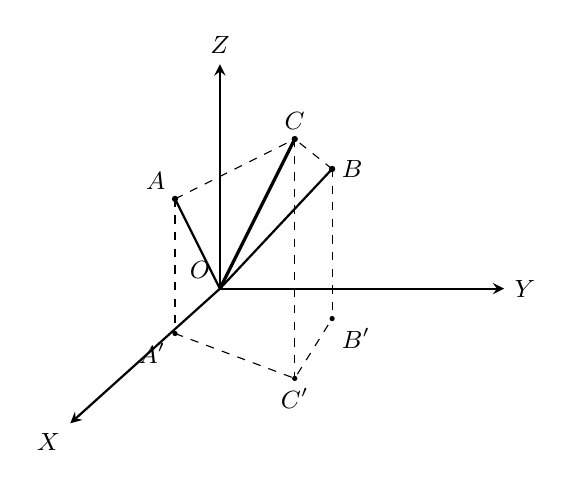
\begin{tikzpicture}[>=stealth, scale=0.95, font=\small]
  \draw[->, thick] (0, 0) -- (-2, -1.8) node[below left] {$X$};
  \draw[->, thick] (0, 0) -- (3.8, 0) node[right] {$Y$};
  \draw[->, thick] (0, 0) -- (0, 3) node[above] {$Z$};
  \node[above left] at (0, 0) {$O$};

  \coordinate (A) at (-0.6, 1.2);
  \coordinate (B) at (1.5, 1.6);
  \coordinate (C) at (1.0, 2.0);

  \draw[thick] (0, 0) -- (A) node[midway, left] {};
  \draw[thick] (0, 0) -- (B) node[midway, below] {};
  \draw[very thick] (0, 0) -- (C);
  \draw[dashed] (A) -- (C);
  \draw[dashed] (B) -- (C);

  \fill (A) circle (1.2pt) node[above left] {$A$};
  \fill (B) circle (1.2pt) node[right] {$B$};
  \fill (C) circle (1.2pt) node[above] {$C$};

  % Coordinates in space projection
  \coordinate (Aprime) at (-0.6, -0.6);
  \coordinate (Bprime) at (1.5, -0.4);
  \coordinate (Cprime) at (1.0, -1.2);

  \draw[dashed] (A) -- (Aprime);
  \draw[dashed] (B) -- (Bprime);
  \draw[dashed] (C) -- (Cprime);
  \draw[dashed] (Aprime) -- (Cprime) -- (Bprime);

  \fill (Aprime) circle (1pt) node[below left] {$A'$};
  \fill (Bprime) circle (1pt) node[below right] {$B'$};
  \fill (Cprime) circle (1pt) node[below] {$C'$};
\end{tikzpicture}
\caption{空間向量加減之投影長方圖解}
\label{fig:b3-fig3-23}
\end{figure}

% =========================================================================
% § 3-4 向量的係數積
% =========================================================================
\subsection{向量的係數積}
\label{sec:b3-3-4}

\subsubsection*{甲、係數積的幾何意義}

向量的係數積便是要定義「向量的實數倍」這一觀念. 設任給一向量 $\mathbf{a}$ 及實數 $\alpha$，要考慮 $\mathbf{a}$ 的 $\alpha$ 倍，以 $\alpha\mathbf{a}$ 表示. 我們這樣來定義：

\phantomsection\label{note:b3-ch3-p93-fig-ref}%
\begin{definition}
當 $\alpha \ge 0$ 時，$\alpha\mathbf{a}$ 為一個沿著 $\mathbf{a}$ 的方向走 $|\mathbf{a}|$ 的 $\alpha$ 倍距離的移動，所決定出來的向量.（見圖 3-24-1\footnote{【校訂註】原書此處印作「（見圖 3-25-1）」與「（見圖 3-25-2）」，次頁對應插圖標記為「圖 3-24-1」與「圖 3-24-2」。正文保留原書字樣並在此校記。}）

當 $\alpha < 0$ 時，$\alpha\mathbf{a}$ 為一個逆著 $\mathbf{a}$ 的方向走 $|\mathbf{a}|$ 的 $|\alpha|$ 倍距離的移動，所決定出來的向量.（見圖 3-24-2）
\end{definition}

\begin{figure}[H]
\centering
\begin{minipage}{0.48\textwidth}
\centering
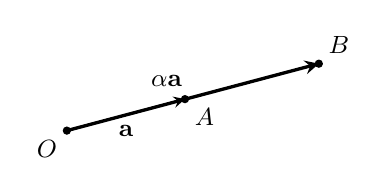
\begin{tikzpicture}[>=stealth, scale=1.0, font=\small]
  \coordinate (O) at (0, 0);
  \coordinate (A) at (1.5, 0.4);
  \coordinate (B) at (3.2, 0.85);

  \draw[->, thick] (O) -- (A) node[midway, below] {$\mathbf{a}$};
  \draw[->, very thick] (O) -- (B) node[midway, above left] {$\alpha\mathbf{a}$};

  \fill (O) circle (1.5pt) node[below left] {$O$};
  \fill (A) circle (1.5pt) node[below right] {$A$};
  \fill (B) circle (1.5pt) node[above right] {$B$};
\end{tikzpicture}
\caption*{當 $\alpha \ge 0$ 時，$\alpha\mathbf{a} = \vec{OB}$\footnote{\phantomsection\label{note:b3-ch3-p94-alpha-c-typo}【校訂註】原書此處插圖說明印作「$c.\mathbf{a} = \vec{OB}$」，「$c.$」顯為純量係數「$\alpha$」之印刷訛字。正文照原書字樣錄入。}，其中 $\overline{OB} = \alpha\cdot\overline{OA}$}
\caption{係數積幾何意義（$\alpha \ge 0$）}
\label{fig:b3-fig3-24-1}
\end{minipage}
\hfill
\begin{minipage}{0.48\textwidth}
\centering
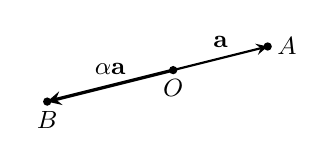
\begin{tikzpicture}[>=stealth, scale=1.0, font=\small]
  \coordinate (O) at (1.8, 0.5);
  \coordinate (A) at (3.0, 0.8);
  \coordinate (B) at (0.2, 0.1);

  \draw[->, thick] (O) -- (A) node[midway, above] {$\mathbf{a}$};
  \draw[->, very thick] (O) -- (B) node[midway, above] {$\alpha\mathbf{a}$};

  \fill (O) circle (1.5pt) node[below] {$O$};
  \fill (A) circle (1.5pt) node[right] {$A$};
  \fill (B) circle (1.5pt) node[below] {$B$};
\end{tikzpicture}
\caption*{當 $\alpha < 0$ 時，$\alpha\mathbf{a} = \vec{OB}$，其中 $\overline{OB} = |\alpha|\cdot\overline{OA}$}
\caption{係數積幾何意義（$\alpha < 0$）}
\label{fig:b3-fig3-24-2}
\end{minipage}
\end{figure}

我們稱 $\alpha\mathbf{a}$ 為實數 $\alpha$ 與向量 $\mathbf{a}$ 的係數積.

特別地，我們容易證得（證明留做習題）以下兩件事：
\begin{enumerate}[label=(\roman*), leftmargin=2.5em]
  \item 當 $\alpha$ 為正整數 $n$ 時，係數積 $n\mathbf{a}$ 正好等於 $n$ 個 $\mathbf{a}$，根據向量加法加在一起，亦即
  \[ n\mathbf{a} = \underbrace{\mathbf{a} + \mathbf{a} + \dots + \mathbf{a}}_{n\text{ 個 }\mathbf{a}} \]
  \item 當 $\alpha = -1$，係數積 $(-1)\mathbf{a}$ 正好就是 $\mathbf{a}$ 的逆向量，亦即
  \[ (-1)\mathbf{a} = -\mathbf{a} \]
\end{enumerate}

\begin{example}
給定二向量 $\mathbf{a}, \mathbf{b}$，取 $\vec{OC} = \frac{3}{2}\mathbf{a} - \mathbf{b}, \vec{OD} = \mathbf{b} - \frac{3}{4}\mathbf{a}$，圖示 $\Delta OCD$，並求代表第三邊的一個有向線段 $\vec{CD}$：
其中
\begin{align*}
\vec{OA} &= \mathbf{a} \\
\vec{OB} &= \mathbf{b} \\
\vec{OC} &= \frac{3}{2}\mathbf{a} - \mathbf{b} \\
\vec{OD} &= \mathbf{b} - \frac{3}{4}\mathbf{a}
\end{align*}
\end{example}

\begin{figure}[H]
\centering
\begin{tikzpicture}[>=stealth, scale=1.0, font=\small]
  \coordinate (O) at (0, 0);
  \coordinate (A) at (2.2, 0.4);
  \coordinate (B) at (1.0, 2.0);

  % C = 1.5 a - b = (3.3 - 1.0, 0.6 - 2.0) = (2.3, -1.4)
  \coordinate (C) at ($(1.5, 0.27) - (1.0, 2.0) + (1.8, 0.33)$);
  % D = b - 0.75 a = (1.0 - 1.65, 2.0 - 0.3) = (-0.65, 1.7)
  \coordinate (D) at ($(-0.65, 1.7)$);

  \draw[->, thick] (O) -- (A) node[midway, above] {$\mathbf{a}$};
  \draw[->, thick] (O) -- (B) node[midway, left] {$\mathbf{b}$};
  \draw[->, very thick] (O) -- (C);
  \draw[->, very thick] (O) -- (D);
  \draw[thick] (C) -- (D);
  \draw[dashed] (B) -- (D);
  \draw[dashed] (A) -- (C);

  \fill (O) circle (1.5pt) node[below left] {$O$};
  \fill (A) circle (1.5pt) node[above right] {$A$};
  \fill (B) circle (1.5pt) node[above] {$B$};
  \fill (C) circle (1.5pt) node[below right] {$C$};
  \fill (D) circle (1.5pt) node[above left] {$D$};
\end{tikzpicture}
\caption{向量組合圖解}
\label{fig:b3-fig3-25}
\end{figure}

\begin{proof}[解]
\phantomsection\label{note:b3-ch3-p95-ex2-ref}%
由 §3-3 丁中論例 2\footnote{【校訂註】原書排印作「由 §3-2 丁中論例 2」，實指 § 3-3 丁中論例 2（頁 90，$\vec{AB} = \mathbf{b} - \mathbf{a}$）。又下文原印「而由圖 3-26，易知」，該題插圖實為本頁上方「圖 3-25」。正文保留原書字樣並在此校記。}，知
\[ \vec{CD} = \vec{OD} - \vec{OC} = \left(\mathbf{b} - \frac{3}{4}\mathbf{a}\right) - \left(\frac{3}{2}\mathbf{a} - \mathbf{b}\right) \]
而由圖 3-25，易知
\[ \vec{CD} = 2\mathbf{b} - \frac{9}{4}\mathbf{a}. \qedhere \]
\end{proof}

\subsubsection*{作業 3}
\begin{enumerate}[label=(\roman*), leftmargin=2em]
  \item 設 $\mathbf{a}, \mathbf{b}$ 為給定的兩向量，取 $\vec{OC} = 2\mathbf{a} - \frac{7}{5}\mathbf{b}, \vec{OD} = -\mathbf{a} - 2\mathbf{b}$，畫出平行四邊形 $OCED$，並求代表 $\vec{OE}, \vec{CD}$ 之向量（以 $\mathbf{a}, \mathbf{b}$ 表之）.
  \item 設 $\mathbf{a}, \mathbf{b}, \mathbf{c}$ 為給定的三向量，考慮折線 $AB \cup BC \cup CD \cup DE$. 設 $\vec{AB} = \mathbf{a} - \mathbf{c}, \vec{BC} = 2\mathbf{a} - \mathbf{b} + \frac{2}{3}\mathbf{c}, \vec{CD} = -\mathbf{b} + \mathbf{c}, \vec{DE} = \mathbf{a} + \mathbf{b} + \mathbf{c}$. 繪圖並求 $\vec{DB}, \vec{AE}, \vec{CA}$ 所代表之向量（以 $\mathbf{a}, \mathbf{b}, \mathbf{c}$ 表之）.
\end{enumerate}

\subsubsection*{乙、係數積的座標成分表示}

由簡單的相似形原理，我們看出：
\begin{theorem}
若 $\mathbf{a} = (x, y, z)$，則
\[ \alpha\mathbf{a} = (\alpha x, \alpha y, \alpha z). \]
\end{theorem}

\begin{figure}[H]
\centering
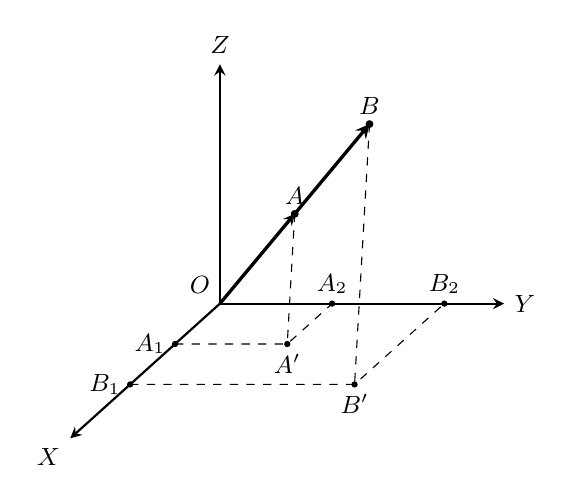
\begin{tikzpicture}[>=stealth, scale=0.95, font=\small]
  \draw[->, thick] (0, 0) -- (-2, -1.8) node[below left] {$X$};
  \draw[->, thick] (0, 0) -- (3.8, 0) node[right] {$Y$};
  \draw[->, thick] (0, 0) -- (0, 3.2) node[above] {$Z$};
  \node[above left] at (0, 0) {$O$};

  \coordinate (A) at (1.0, 1.2);
  \coordinate (B) at (2.0, 2.4);

  \draw[->, thick] (0, 0) -- (A) node[midway, left] {};
  \draw[->, very thick] (0, 0) -- (B) node[midway, above left] {};

  \coordinate (A1) at (-0.6, -0.54);
  \coordinate (A2) at (1.5, 0);
  \coordinate (Aprime) at (0.9, -0.54);

  \coordinate (B1) at (-1.2, -1.08);
  \coordinate (B2) at (3.0, 0);
  \coordinate (Bprime) at (1.8, -1.08);

  \draw[dashed] (A) -- (Aprime);
  \draw[dashed] (B) -- (Bprime);
  \draw[dashed] (A1) -- (Aprime) -- (A2);
  \draw[dashed] (B1) -- (Bprime) -- (B2);

  \fill (A) circle (1.5pt) node[above] {$A$};
  \fill (B) circle (1.5pt) node[above] {$B$};
  \fill (A1) circle (1.2pt) node[left] {$A_1$};
  \fill (A2) circle (1.2pt) node[above] {$A_2$};
  \fill (B1) circle (1.2pt) node[left] {$B_1$};
  \fill (B2) circle (1.2pt) node[above] {$B_2$};
  \fill (Aprime) circle (1.2pt) node[below] {$A'$};
  \fill (Bprime) circle (1.2pt) node[below] {$B'$};
\end{tikzpicture}
\caption{係數積之空間相似形投影}
\label{fig:b3-fig3-26}
\end{figure}

\begin{proof}
設 $\vec{OB} = \alpha\mathbf{a} = (x', y', z')$，則
\begin{align*}
\frac{x'}{x} &= \pm \frac{\overline{OB_1}}{\overline{OA_1}} \quad \text{〔正、負號依 $A_1$ 與 $B_1$ 在 $O$ 之同、異側而定〕} \\
&= \pm \frac{\overline{OB'}}{\overline{OA'}} \quad \text{〔正、負號依 $A'$ 與 $B'$ 在 $O$ 之同、異側而定〕} \\
&= \pm \frac{\overline{OB}}{\overline{OA}} \quad \text{〔正、負號依 $A$ 與 $B$ 在 $O$ 之同、異側而定〕} \\
&= \alpha
\end{align*}
故 $x' = \alpha x$，同理可得 $y' = \alpha y, z' = \alpha z$.
亦即
\[ \alpha\mathbf{a} = (\alpha x, \alpha y, \alpha z). \qedhere \]
\end{proof}

\subsubsection*{丙、係數積的基本性質}

利用座標成分來表示向量的運算，如加法、係數積等，的好處在於可以很快地檢驗是否有一些實數系中相應的運算性質能被搬到向量上面來. 譬如，我們雖已在 §3-3 由幾何意義證明了加法交換律，但若利用座標成分來看向量加法，則知：因交換律在實數系的每一座標成分上是正確的，所以在向量上也是正確的. 詳述如下：

設 $\mathbf{a} = (x_1, y_1, z_1), \mathbf{b} = (x_2, y_2, z_2)$，則
\begin{align*}
\mathbf{a} + \mathbf{b} &= (x_1 + x_2, y_1 + y_2, z_1 + z_2) \\
&= (x_2 + x_1, y_2 + y_1, z_2 + z_1) = \mathbf{b} + \mathbf{a}. \quad \#
\end{align*}

現在，我們也就是要利用這樣的座標成分分解的觀點來推證下列基本性質：

\begin{proposition}
\begin{enumerate}[label=(\Roman*), leftmargin=2em]
  \item $\alpha(\mathbf{a} + \mathbf{b}) = \alpha\mathbf{a} + \alpha\mathbf{b}$
  \item $(\alpha + \beta)\mathbf{a} = \alpha\mathbf{a} + \beta\mathbf{a}$
  \item $(\alpha\beta)\mathbf{a} = \alpha(\beta\mathbf{a})$
\end{enumerate}
其中 $\alpha, \beta \in \mathbb{R}$，$\mathbf{a}, \mathbf{b}$ 為任意兩向量.
\end{proposition}

\begin{proof}
設 $\mathbf{a} = (x_1, y_1, z_1), \mathbf{b} = (x_2, y_2, z_2)$，則
\[ \mathbf{a} + \mathbf{b} = (x_1 + x_2, y_1 + y_2, z_1 + z_2) \]

(I)
\begin{align*}
\alpha(\mathbf{a} + \mathbf{b}) &= (\alpha(x_1 + x_2), \alpha(y_1 + y_2), \alpha(z_1 + z_2)) \quad \text{〔係數積成分表示〕} \\
&= (\alpha x_1 + \alpha x_2, \alpha y_1 + \alpha y_2, \alpha z_1 + \alpha z_2) \quad \text{〔實數系分配律〕} \\
&= (\alpha x_1, \alpha y_1, \alpha z_1) + (\alpha x_2, \alpha y_2, \alpha z_2) \quad \text{〔向量加法成分表示〕} \\
&= \alpha\mathbf{a} + \alpha\mathbf{b} \quad \text{〔係數積成分表示〕}
\end{align*}

(II)
\begin{align*}
(\alpha + \beta)\mathbf{a} &= ((\alpha + \beta)x_1, (\alpha + \beta)y_1, (\alpha + \beta)z_1) \quad \text{〔係數積成分表示〕} \\
&= (\alpha x_1 + \beta x_1, \alpha y_1 + \beta y_1, \alpha z_1 + \beta z_1) \quad \text{〔實數系分配律〕} \\
&= (\alpha x_1, \alpha y_1, \alpha z_1) + (\beta x_1, \beta y_1, \beta z_1) \quad \text{〔向量加法成分表示〕} \\
&= \alpha\mathbf{a} + \beta\mathbf{a} \quad \text{〔係數積成分表示〕}
\end{align*}

(III) 留當作業. \qedhere
\end{proof}

我們用圖解來說明這些基本性質：

(I) 設 $\mathbf{a} = \vec{OA}, \mathbf{b} = \vec{OB} = \vec{AC}, \alpha\mathbf{a} = \vec{OA'}, \alpha\mathbf{b} = \vec{OB'} = \vec{A'C'}$.
則知 $\mathbf{a} + \mathbf{b} = \vec{OC}, \alpha\mathbf{a} + \alpha\mathbf{b} = \vec{OC'}$.

\begin{figure}[H]
\centering
\begin{minipage}{0.48\textwidth}
\centering
\begin{tikzpicture}[>=stealth, scale=0.85, font=\small]
  \coordinate (O) at (0, 0);
  \coordinate (A) at (1.5, 0.2);
  \coordinate (B) at (0.8, 0.9);
  \coordinate (C) at ($(A) + (B)$);

  \coordinate (Aprime) at (3.0, 0.4);
  \coordinate (Bprime) at (1.6, 1.8);
  \coordinate (Cprime) at ($(Aprime) + (Bprime)$);

  \draw[->, thick] (O) -- (A) node[midway, below] {$\mathbf{a}$};
  \draw[->, thick] (O) -- (B) node[midway, left] {$\mathbf{b}$};
  \draw[->, thick] (O) -- (C) node[midway, below right] {$\mathbf{a}+\mathbf{b}$};
  \draw[dashed] (A) -- (C);

  \draw[->, very thick] (O) -- (Aprime) node[midway, below] {$\alpha\mathbf{a}$};
  \draw[->, very thick] (O) -- (Bprime) node[midway, left] {$\alpha\mathbf{b}$};
  \draw[->, very thick] (O) -- (Cprime) node[midway, above left, sloped] {$\alpha(\mathbf{a}+\mathbf{b})=\alpha\mathbf{a}+\alpha\mathbf{b}$};
  \draw[dashed] (Aprime) -- (Cprime);

  \fill (O) circle (1.2pt) node[left] {$O$};
  \fill (A) circle (1.2pt) node[below] {$A$};
  \fill (B) circle (1.2pt) node[above left] {$B$};
  \fill (C) circle (1.2pt) node[right] {$C$};
  \fill (Aprime) circle (1.2pt) node[below] {$A'$};
  \fill (Bprime) circle (1.2pt) node[above left] {$B'$};
  \fill (Cprime) circle (1.2pt) node[above right] {$C'$};
\end{tikzpicture}
\caption*{當 $\alpha > 0$ 時}
\caption{係數積分配律圖解（$\alpha > 0$）}
\label{fig:b3-fig3-27-1}
\end{minipage}
\hfill
\begin{minipage}{0.48\textwidth}
\centering
\begin{tikzpicture}[>=stealth, scale=0.85, font=\small]
  \coordinate (O) at (0, 0);
  \coordinate (A) at (1.5, 0.3);
  \coordinate (B) at (0.6, 1.2);
  \coordinate (C) at ($(A) + (B)$);

  \coordinate (Aprime) at (-1.8, -0.36);
  \coordinate (Bprime) at (-0.72, -1.44);
  \coordinate (Cprime) at ($(Aprime) + (Bprime)$);

  \draw[->, thick] (O) -- (A) node[midway, below] {$\mathbf{a}$};
  \draw[->, thick] (O) -- (B) node[midway, left] {$\mathbf{b}$};
  \draw[->, thick] (O) -- (C);
  \draw[dashed] (A) -- (C);

  \draw[->, very thick] (O) -- (Aprime) node[midway, above left] {$\alpha\mathbf{a}$};
  \draw[->, very thick] (O) -- (Bprime) node[midway, right] {$\alpha\mathbf{b}$};
  \draw[->, very thick] (O) -- (Cprime);
  \draw[dashed] (Aprime) -- (Cprime);

  \fill (O) circle (1.2pt) node[above] {$O$};
  \fill (A) circle (1.2pt) node[right] {$A$};
  \fill (B) circle (1.2pt) node[above] {$B$};
  \fill (C) circle (1.2pt) node[right] {$C$};
  \fill (Aprime) circle (1.2pt) node[above left] {$A'$};
  \fill (Bprime) circle (1.2pt) node[right] {$B'$};
  \fill (Cprime) circle (1.2pt) node[below left] {$C'$};
\end{tikzpicture}
\caption*{當 $\alpha < 0$ 時}
\caption{係數積分配律圖解（$\alpha < 0$）}
\label{fig:b3-fig3-27-2}
\end{minipage}
\end{figure}

另一方面，
\[ \frac{\overline{OC'}}{\overline{OC}} = \frac{\overline{OA'}}{\overline{OA}} \quad \text{〔因 } AC \parallel A'C'\text{〕} = \pm \alpha \quad \text{〔正、負號依 $\alpha$ 之正負而定〕} \]
故 $\vec{OC'}$ 代表 $\alpha(\mathbf{a} + \mathbf{b})$. 即
\[ \alpha(\mathbf{a} + \mathbf{b}) = \alpha\mathbf{a} + \alpha\mathbf{b} \]
也就是兩向量和的某實數倍，等於兩向量的該實數倍的和，這其實就是相似三角形原理.

(II) 設 $\mathbf{a} = \vec{OA}, \alpha\mathbf{a} = \vec{OA_1}, \beta\mathbf{a} = \vec{OA_2}$. 今取一有向線段 $\vec{A_1 A_3}$，使
\[ \beta\mathbf{a} = \vec{A_1 A_3} \]
則因 $\vec{OA_1}$ 與 $\vec{A_1 A_3}$ 首尾相接，故：
\[ \alpha\mathbf{a} + \beta\mathbf{a} = \vec{OA_1} + \vec{A_1 A_3} = \vec{OA_3} \]
$\vec{OA_3}$ 為自 $O$ 沿 $\mathbf{a}$ 的方向走 $|\mathbf{a}|$ 的 $\alpha$ 倍，再走 $\beta$ 倍（方向各依 $\alpha, \beta$ 之正負而定）. 故其實就是沿 $\mathbf{a}$ 的方向走 $\alpha + \beta$ 倍（方向依 $\alpha + \beta$ 之正負而定）. 因此 $\vec{OA_3} = (\alpha + \beta)\mathbf{a}$，即
\[ \alpha\mathbf{a} + \beta\mathbf{a} = (\alpha + \beta)\mathbf{a}. \]

\begin{figure}[H]
\centering
\begin{minipage}{0.48\textwidth}
\centering
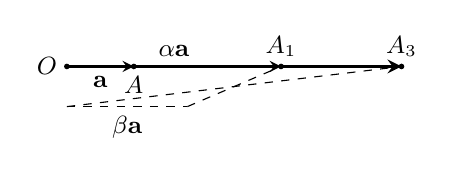
\begin{tikzpicture}[>=stealth, scale=0.85, font=\small]
  \coordinate (O) at (0, 0);
  \coordinate (A) at (1.0, 0);
  \coordinate (A1) at (3.2, 0);
  \coordinate (A3) at (5.0, 0);

  \draw[->, thick] (O) -- (A) node[midway, below] {$\mathbf{a}$};
  \draw[->, thick] (O) -- (A1) node[midway, above] {$\alpha\mathbf{a}$};
  \draw[->, very thick] (A1) -- (A3);

  \draw[dashed] (0, -0.6) -- (1.8, -0.6) node[midway, below] {$\beta\mathbf{a}$};
  \draw[dashed] (1.8, -0.6) -- (A1);
  \draw[dashed] (0, -0.6) -- (A3);

  \fill (O) circle (1.2pt) node[left] {$O$};
  \fill (A) circle (1.2pt) node[below] {$A$};
  \fill (A1) circle (1.2pt) node[above] {$A_1$};
  \fill (A3) circle (1.2pt) node[above] {$A_3$};
\end{tikzpicture}
\caption{係數和分配律（同號情形）}
\label{fig:b3-fig3-28-1}
\end{minipage}
\hfill
\begin{minipage}{0.48\textwidth}
\centering
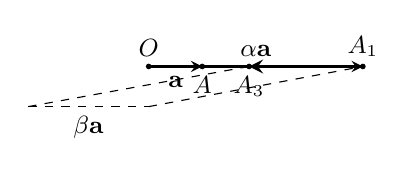
\begin{tikzpicture}[>=stealth, scale=0.85, font=\small]
  \coordinate (O) at (2.0, 0);
  \coordinate (A) at (2.8, 0);
  \coordinate (A1) at (5.2, 0);
  \coordinate (A3) at (3.5, 0);

  \draw[->, thick] (O) -- (A) node[midway, below] {$\mathbf{a}$};
  \draw[->, thick] (O) -- (A1) node[midway, above] {$\alpha\mathbf{a}$};
  \draw[->, very thick] (A1) -- (A3);

  \draw[dashed] (0.2, -0.6) -- (2.0, -0.6) node[midway, below] {$\beta\mathbf{a}$};
  \draw[dashed] (0.2, -0.6) -- (A3);
  \draw[dashed] (2.0, -0.6) -- (A1);

  \fill (O) circle (1.2pt) node[above] {$O$};
  \fill (A) circle (1.2pt) node[below] {$A$};
  \fill (A1) circle (1.2pt) node[above] {$A_1$};
  \fill (A3) circle (1.2pt) node[below] {$A_3$};
\end{tikzpicture}
\caption{係數和分配律（異號情形）}
\label{fig:b3-fig3-28-2}
\end{minipage}
\end{figure}

(III) 留當作業.

\subsubsection*{作業 4}
證明 $(\alpha\beta)\mathbf{a} = \alpha(\beta\mathbf{a})$ 並仿本文以圖解說明.

\begin{example}[論例 6]
取空間中三點 $P(2, 0, 1), Q(3, 1, -1)$ 與 $R(1, 1, 2)$. 設向量 $\mathbf{a} = \vec{PQ} - 2\cdot\vec{QR}$ 其中 $2\cdot\vec{QR}$ 表係數積，求 $\mathbf{a}$ 的座標表示，並問從 $A(5, 3, -7)$ 引一有向線段 $\vec{AB}$，使 $\vec{AB} = -2\mathbf{a}$，則 $B$ 點座標座落何處？
\end{example}

\begin{proof}[解]
這論例要顯示出：我們從幾何觀點定義出來的向量一經賦予座標後，便可以純用運算代替幾何的作圖. 這樣的方法簡捷而有系統，能夠這樣是基於加法與係數積等向量運算之座標表示.

運算如下：
\begin{align*}
\vec{PQ} &= \vec{OQ} - \vec{OP} = (3, 1, -1) - (2, 0, 1) = (1, 1, -2) \\
\vec{QR} &= \vec{OR} - \vec{OQ} = (1, 1, 2) - (3, 1, -1) = (-2, 0, 3)\footnotemark
\end{align*}
\footnotetext{\phantomsection\label{note:b3-ch3-p100-qr-typo}【校訂註】原書此處印作 $(\quad 3, 0, 3)$，負號與數字 2 印刷模糊脫落，依前後文計算校訂為 $(-2, 0, 3)$。}
故
\begin{align*}
\mathbf{a} &= \vec{PQ} - 2\cdot\vec{QR} = (1, 1, -2) - 2\cdot(-2, 0, 3) \\
&= (1, 1, -2) - (-4, 0, 6) = (5, 1, -8)
\end{align*}
即 $\mathbf{a}$ 的座標表示為 $(5, 1, -8)$.

又
\[ \vec{AB} = -2\mathbf{a} = (-2)\cdot(5, 1, -8) = (-10, -2, 16) \]
但 $A$ 座標為 $(5, 3, -7)$，故
\[ \vec{OB} = \vec{OA} + \vec{AB} = (-5, 1, 9) \]
即 $B$ 點座標為 $(-5, 1, 9)$. \qedhere
\end{proof}

\subsubsection*{作業 5}
\begin{enumerate}[label=(\roman*), leftmargin=2em]
  \item 畫圖驗證上述論例之結果.（立體圖）
  \item 設空間中四點 $P(1, 3, 1), Q(0, -1, 3), R(1, 1, 1), S(1, -1, 4)$. 設向量 $\mathbf{a} = \frac{1}{2}\vec{PQ} - \vec{RP} + 2\vec{QS}$. 今有一有向線段 $\vec{AB}$ 代表 $3\mathbf{a}$，即 $3\mathbf{a} = \vec{AB}$，知 $B$ 點為 $(10, 5, 2)$，問 $A$ 點座標落何處？
\end{enumerate}

\begin{example}[論例 7]
$\Delta ABC$ 為一三角形，$O$ 為任一點. 令 $\mathbf{a} = \vec{OA}, \mathbf{b} = \vec{OB}, \mathbf{c} = \vec{OC}$，設 $D, E, F$ 分別為 $\overline{BC}, \overline{CA}, \overline{AB}$ 各邊中點，則
\[ \vec{OD} = \frac{1}{2}(\mathbf{b} + \mathbf{c}), \quad \vec{OE} = \frac{1}{2}(\mathbf{c} + \mathbf{a}), \quad \vec{OF} = \frac{1}{2}(\mathbf{a} + \mathbf{b}). \]
\end{example}

\begin{proof}
做 $\square OCHB$，則 $D$ 為 $\overline{OH}$ 中點. 即
\[ \vec{OD} = \vec{DH} = \frac{1}{2}\vec{OH} \]
今
\[ \vec{OH} = \vec{OC} + \vec{OB} = \mathbf{c} + \mathbf{b} \]
故
\[ \vec{OD} = \frac{1}{2}(\mathbf{b} + \mathbf{c}). \]
另二式同法可證. \qedhere
\end{proof}

\begin{figure}[H]
\centering
\begin{tikzpicture}[>=stealth, scale=0.95, font=\small]
  \coordinate (O) at (1.5, 0.8);
  \coordinate (A) at (1.5, 3.2);
  \coordinate (B) at (0, 0.6);
  \coordinate (C) at (3.2, 0.6);

  \coordinate (D) at ($(B)!0.5!(C)$);
  \coordinate (E) at ($(C)!0.5!(A)$);
  \coordinate (F) at ($(A)!0.5!(B)$);
  \coordinate (H) at ($(C) + (B) - (O)$);

  \draw[thick] (A) -- (B) -- (C) -- cycle;
  \draw[dashed] (O) -- (A);
  \draw[dashed] (O) -- (B);
  \draw[dashed] (O) -- (C);
  \draw[very thick] (O) -- (D);
  \draw[thick] (B) -- (H) -- (C);
  \draw[dashed] (O) -- (H);

  \fill (O) circle (1.5pt) node[right] {$O$};
  \fill (A) circle (1.5pt) node[above] {$A$};
  \fill (B) circle (1.5pt) node[left] {$B$};
  \fill (C) circle (1.5pt) node[right] {$C$};
  \fill (D) circle (1.2pt) node[above right] {$D$};
  \fill (E) circle (1.2pt) node[above right] {$E$};
  \fill (F) circle (1.2pt) node[above left] {$F$};
  \fill (H) circle (1.2pt) node[below] {$H$};
\end{tikzpicture}
\caption{三角形邊中點之向量表示}
\label{fig:b3-fig3-29}
\end{figure}

\begin{example}[論例 8 （重心定理）]
設 $G$ 為 $\Delta ABC$ 中線 $AD$ 上滿足 $\overline{AG} = 2\overline{GD}$ 之一點，$O$ 為空間中任取之點，設 $\mathbf{a} = \vec{OA}, \mathbf{b} = \vec{OB}, \mathbf{c} = \vec{OC}$，證明
\[ \vec{OG} = \frac{1}{3}(\mathbf{a} + \mathbf{b} + \mathbf{c}). \]
\end{example}

\begin{proof}
\phantomsection\label{note:b3-ch3-p102-ge-typo}%
如果這式成立，同樣取 $G', G''$ 為其他兩中線 $BE, CF$ 上分別滿足 $\overline{BG'} = 2\overline{G'E}, \overline{CG''} = 2\overline{G''F}$\footnote{【校訂註】原書第 2 行印作「$\overline{CG''} = 2\overline{G''E}$ 之點」，因 $G''$ 為中線 $CF$ 上之點，右端「$E$」實為「$F$」之排印訛字。正文照原書字樣錄入並在此校記。} 之點. 則亦得證知
\begin{align*}
\vec{OG'} &= \frac{1}{3}(\mathbf{a} + \mathbf{b} + \mathbf{c}) \\
\vec{OG''} &= \frac{1}{3}(\mathbf{a} + \mathbf{b} + \mathbf{c})
\end{align*}
因此三個同自始點 $O$ 出發之有向線段 $\vec{OG}, \vec{OG'}, \vec{OG''}$ 代表同一向量 $\frac{1}{3}(\mathbf{a} + \mathbf{b} + \mathbf{c})$，故知
\[ G, G', G'' \text{ 重合為一點} \]
亦即 $\Delta ABC$ 三中線交會於一點，（這點稱為重心）此稱為三角形重心定理.

\begin{figure}[H]
\centering
\begin{minipage}{0.48\textwidth}
\centering
\begin{tikzpicture}[>=stealth, scale=0.85, font=\small]
  \coordinate (A) at (1.5, 3.0);
  \coordinate (B) at (0, 0.4);
  \coordinate (C) at (3.5, 0.8);

  \coordinate (D) at ($(B)!0.5!(C)$);
  \coordinate (E) at ($(C)!0.5!(A)$);
  \coordinate (F) at ($(A)!0.5!(B)$);
  \coordinate (G) at (barycentric cs:A=1,B=1,C=1);

  \draw[thick] (A) -- (B) -- (C) -- cycle;
  \draw[thick] (A) -- (D);
  \draw[thick] (B) -- (E);
  \draw[thick] (C) -- (F);

  \fill (A) circle (1.2pt) node[above] {$A$};
  \fill (B) circle (1.2pt) node[left] {$B$};
  \fill (C) circle (1.2pt) node[right] {$C$};
  \fill (D) circle (1.2pt) node[below] {$D$};
  \fill (E) circle (1.2pt) node[above right] {$E$};
  \fill (F) circle (1.2pt) node[above left] {$F$};
  \fill (G) circle (1.5pt) node[below] {$G$};
  \node[right] at (G) {\scriptsize $G', G''$};
\end{tikzpicture}
\caption{三中線共點於重心}
\label{fig:b3-fig3-30}
\end{minipage}
\hfill
\begin{minipage}{0.48\textwidth}
\centering
\begin{tikzpicture}[>=stealth, scale=0.85, font=\small]
  \coordinate (O) at (0.2, 3.2);
  \coordinate (A) at (2.2, 3.2);
  \coordinate (B) at (0.0, 0.4);
  \coordinate (C) at (3.5, 0.8);

  \coordinate (D) at ($(B)!0.5!(C)$);
  \coordinate (G) at (barycentric cs:A=1,B=1,C=1);

  \draw[thick] (A) -- (B) -- (C) -- cycle;
  \draw[thick] (A) -- (D);

  \draw[very thick, ->] (O) -- (A) node[midway, above] {$\mathbf{a}$};
  \draw[very thick, ->] (O) -- (B) node[midway, left] {$\mathbf{b}$};
  \draw[very thick, ->] (O) -- (C) node[midway, above right] {$\mathbf{c}$};
  \draw[very thick, ->] (O) -- (G) node[midway, above right] {};

  \fill (O) circle (1.5pt) node[left] {$O$};
  \fill (A) circle (1.2pt) node[above] {$A$};
  \fill (B) circle (1.2pt) node[left] {$B$};
  \fill (C) circle (1.2pt) node[right] {$C$};
  \fill (D) circle (1.2pt) node[below] {$D$};
  \fill (G) circle (1.5pt) node[right] {$G$};
\end{tikzpicture}
\caption{重心之向量表示}
\label{fig:b3-fig3-31}
\end{minipage}
\end{figure}

現在回來證明 $\vec{OG} = \frac{1}{3}(\mathbf{a} + \mathbf{b} + \mathbf{c})$：方法是根據向量加法、係數積，把 $\vec{OG}$ 逐步拆解，使最後表成 $\mathbf{a}, \mathbf{b}, \mathbf{c}$.
\begin{align*}
\vec{OG} &= \vec{OA} + \vec{AG} = \vec{OA} + \frac{2}{3}\vec{AD} = \vec{OA} + \frac{2}{3}(\vec{AO} + \vec{OD}) \\
&= \vec{OA} + \frac{2}{3}\left(-\vec{OA} + \frac{1}{2}(\vec{OB} + \vec{OC})\right) \quad \text{〔根據論例 7〕} \\
&= \left(1 - \frac{2}{3}\right)\vec{OA} + \frac{1}{3}\vec{OB} + \frac{1}{3}\vec{OC} \\
&= \frac{1}{3}(\mathbf{a} + \mathbf{b} + \mathbf{c}) \quad \text{故得證.} \qedhere
\end{align*}
\end{proof}

這個重心定理在第四章時還要作為一個利用座標幾何處理問題的例子來被再證一次.

\subsubsection*{作業 6}
設 $A(1, 2, 1), B(3, 3, 0), C(-1, 1, 1)$，求 $\Delta ABC$ 重心 $G$ 之位置，以座標表出.

\subsubsection*{習題 3-4}

\begin{enumerate}[label=\arabic*., leftmargin=2em]
  \item 設 $\mathbf{a}$ 與 $\mathbf{b}$ 為給定向量，試作圖表示向量 $\mathbf{c}$.
  \begin{enumerate}[label=(\roman*), leftmargin=2em]
    \item $\mathbf{c} = 2\mathbf{a} + \mathbf{b}$
    \item $\mathbf{c} = (-\mathbf{a}) + 2\mathbf{b}$
    \item $\mathbf{c} = 2\mathbf{a} - 3\mathbf{b}$
  \end{enumerate}
  \item 設 $\mathbf{a}, \mathbf{b}, \mathbf{c}$ 為給定向量，試解出下列方程式中之向量 $\mathbf{x}$：
  \begin{enumerate}[label=(\roman*), leftmargin=2em]
    \item $\frac{8}{5}(3\mathbf{a} - 5\mathbf{x}) + 5(3\mathbf{x} - 2\mathbf{b}) = \mathbf{0}$
    \item $2\left(\mathbf{x} - \frac{1}{3}\mathbf{a}\right) - \frac{1}{2}(\mathbf{b} - 3\mathbf{x} + \mathbf{c}) + \mathbf{b} = \mathbf{0}$
  \end{enumerate}
  \item 設 $T$ 為線段 $\overline{AB}$ 上任一點，而 $\mathbf{a} = \vec{AB}$，試證
  \[ \vec{AT} = \frac{\overline{AT}}{\overline{AB}}\mathbf{a}. \]
  \item 設 $m, n$ 不同時為零，試證若 $m\mathbf{a} + n\mathbf{b} = \mathbf{0}, m + n = 0$，則 $\mathbf{a} = \mathbf{b}$.
  \item 令向量 $\mathbf{a} = \vec{AB}, \mathbf{b} = \vec{AC}$，設有向量
  \[ \mathbf{x} = \vec{AT} = t\mathbf{a} + (1 - t)\mathbf{b}, \quad 0 \le t \le 1 \]
  試證 $T$ 在線段 $\overline{BC}$ 上.
  \item 試以歸納法證：$n\mathbf{a} = \underbrace{\mathbf{a} + \mathbf{a} + \dots + \mathbf{a}}_{n\text{ 個}}$，其中 $n \in \mathbb{N}$.
  \item \phantomsection\label{note:b3-ch3-p104-prob7-typo}%
  給定三向量 $\mathbf{a}, \mathbf{b}, \mathbf{c}$，若沿一個四邊形的邊繞行，先依次經過其中連續三邊設這三邊所相應的向量按序為 $2\mathbf{a}, -\mathbf{b} + \frac{1}{2}\mathbf{c}$ 及 $(\mathbf{c} - \mathbf{a})$\footnote{【校訂註】原書此處印作「及 $\text{'' }\mathbf{c}-\mathbf{a}$）時」，標點與引號殘缺倒置，實為「$(\mathbf{c}-\mathbf{a})$」。正文保留原書樣式錄入並在此校記。} 時，試求接下去走第四邊時所相應的向量.
  \item 設 $\Delta ABC$ 三頂點為 $A(1, -1, 2), B(4, -2, 5), C(1, 0, 1)$ 求三條中線長.
  \item 設 $P_1 P_2 \dots P_n$ 為一正 $n$ 邊形而 $O$ 為其中心，試證
  \[ \vec{OP_1} + \vec{OP_2} + \dots + \vec{OP_n} = \mathbf{0}. \]
  〔提示：分解 $\vec{OP_j}$ 為 $\vec{OP_{j+1}}$ 與 $\vec{OP_{j-1}}$ 的組合〕
  \item 設 $\mathbf{a}_1 = \vec{OA_1}, \mathbf{a}_2 = \vec{OA_2}$，則一點 $C$ 在線段 $\overline{A_1 A_2}$ 所相應的向量 $\mathbf{c}$ 可表成
  \begin{align*}
  \mathbf{c} &= \vec{OC} = \vec{OA_1} + \vec{A_1 C} \\
  &= \mathbf{a}_1 + t\vec{A_1 A_2} = \mathbf{a}_1 + t(\mathbf{a}_2 - \mathbf{a}_1) \\
  &= (1 - t)\mathbf{a}_1 + t\mathbf{a}_2 \quad [0 \le t \le 1] \\
  &= \alpha_1\mathbf{a}_1 + \alpha_2\mathbf{a}_2
  \end{align*}
  其中 $\alpha_1 + \alpha_2 = (1 - t) + t = 1, \quad 0 \le \alpha_1, \alpha_2 \le 1$.

  仿此，證明空間中三角形 $A_1 A_2 A_3$ 中的點 $C$ 可表成
  \[ \mathbf{c} = \alpha_1\mathbf{a}_1 + \alpha_2\mathbf{a}_2 + \alpha_3\mathbf{a}_3; \quad 0 \le \alpha_i \le 1 \ \ \forall i \ \text{ 且 } \ \alpha_1 + \alpha_2 + \alpha_3 = 1, \]
  其中 $\mathbf{c} = \vec{OC}, \mathbf{a}_1 = \vec{OA_1}, \mathbf{a}_2 = \vec{OA_2}, \mathbf{a}_3 = \vec{OA_3}$.\\
  〔提示：$\vec{OC} = \vec{OA_1} + \vec{A_1 C}$，但 $\vec{A_1 C} = t\vec{A_1 A_2} + t'\vec{A_1 A_3}$〕
\end{enumerate}

% =========================================================================
% § 3-5 向量的內積
% =========================================================================
\subsection{向量的內積}
\label{sec:b3-3-5}

向量的內積在近代各門數學體系中扮演一個相當決定性的角色，換句話說，它的引入幾乎決定了該門體系的根本構造.

我們現在所討論的向量是在我們生活著的歐氏空間裏，向量的內積也以一定的形式出現. 從某種觀點來看，內積可以看成是一般投影的度量，但更重要義的是：另一方面它的座標成分表示非常簡潔，且易於計算. 在實際問題的處理上，它是一個有力的工具.

其實，向量代數也是在有了內積之後，才真正顯現出它的好處.

\subsubsection*{甲、單位向量與向量的自然分解}

\begin{definition}
長度為 1 的向量，稱為單位向量.
\end{definition}

空間中單位向量（終點）的全體，描出一個球面，稱為單位球（面）. 平面上單位向量（終點）的全體描出一個圓圈，稱為平面上的單位圓. 而一直線上的單位向量只有兩個，它們的終點描出了兩個點.

\begin{figure}[H]
\centering
\begin{minipage}{0.32\textwidth}
\centering
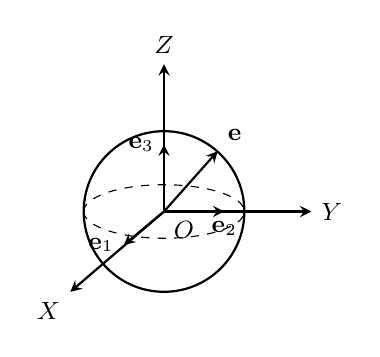
\begin{tikzpicture}[>=stealth, scale=0.85, font=\small]
  \draw[->, thick] (0, 0) -- (-1.4, -1.2) node[below left] {$X$};
  \draw[->, thick] (0, 0) -- (2.2, 0) node[right] {$Y$};
  \draw[->, thick] (0, 0) -- (0, 2.2) node[above] {$Z$};
  \draw[thick] (0, 0) circle (1.2cm);
  \draw[dashed] (-1.2, 0) arc (180:360:1.2 and 0.4);
  \draw[dashed] (-1.2, 0) arc (180:0:1.2 and 0.4);

  \draw[->, thick] (0, 0) -- (0.8, 0.9) node[above right] {$\mathbf{e}$};
  \draw[->, thick] (0, 0) -- (-0.6, -0.5) node[left] {$\mathbf{e}_1$};
  \draw[->, thick] (0, 0) -- (0.9, 0) node[below] {$\mathbf{e}_2$};
  \draw[->, thick] (0, 0) -- (0, 1.0) node[left] {$\mathbf{e}_3$};
  \node[below right] at (0, 0) {$O$};
\end{tikzpicture}
\caption{空間單位球}
\label{fig:b3-fig3-32-1}
\end{minipage}
\hfill
\begin{minipage}{0.32\textwidth}
\centering
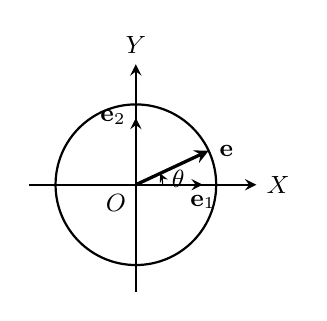
\begin{tikzpicture}[>=stealth, scale=0.85, font=\small]
  \draw[->, thick] (-1.6, 0) -- (1.8, 0) node[right] {$X$};
  \draw[->, thick] (0, -1.6) -- (0, 1.8) node[above] {$Y$};
  \draw[thick] (0, 0) circle (1.2cm);

  \draw[->, very thick] (0, 0) -- (25:1.2) node[right] {$\mathbf{e}$};
  \draw[->, thick] (0, 0) -- (1.0, 0) node[below] {$\mathbf{e}_1$};
  \draw[->, thick] (0, 0) -- (0, 1.0) node[left] {$\mathbf{e}_2$};
  \draw[->] (0.4, 0) arc (0:25:0.4) node[midway, right] {$\theta$};
  \node[below left] at (0, 0) {$O$};
\end{tikzpicture}
\caption{平面單位圓}
\label{fig:b3-fig3-32-2}
\end{minipage}
\hfill
\begin{minipage}{0.32\textwidth}
\centering
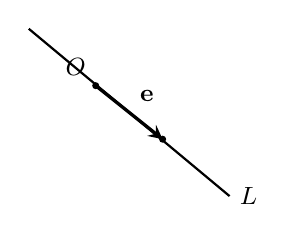
\begin{tikzpicture}[>=stealth, scale=0.85, font=\small]
  \draw[thick] (-0.5, 2.0) -- (2.5, -0.5) node[right] {$L$};
  \coordinate (O) at (0.5, 1.15);
  \coordinate (P) at (1.5, 0.35);

  \draw[->, very thick] (O) -- (P) node[midway, above right] {$\mathbf{e}$};
  \fill (O) circle (1.5pt) node[above left] {$O$};
  \fill (P) circle (1.5pt);
\end{tikzpicture}
\caption{直線上單位向量}
\label{fig:b3-fig3-32-3}
\end{minipage}
\end{figure}

由於空間中的每一方向上都恰好有且只有一個單位向量，我們很多時候便拿單位向量來代表方向. 我們常用單位向量來稱呼它所代表的那個方向，而稱方向 $\mathbf{u}$ 或 $\mathbf{u}$ 的方向，其中 $\mathbf{u}$ 為在那方向上的單位向量.

在空間中一條直線 $L$ 上取定一點 $O$，及一沿 $L$ 的單位向量 $\mathbf{e}$，則 $L$ 上任一點 $P$ 所對應的向量可表成：
\[ \vec{OP} = \alpha\mathbf{e} \]
其中 $\alpha$ 為一實數，可正可負，正負由 $\vec{OP}$ 與 $\mathbf{e}$ 同向或異向而定.

$P$ 點與實數 $\alpha$ 的對應是一對一的，因此，若局限在直線 $L$ 中，則 $L$ 上的點可根據這一對應由一實數來準確地描寫其位置. 這與平面或空間採用座標來描寫點的觀念基本上是一樣的. $\alpha$ 稱為 $P$ 點在 $L$ 上相關於 $(O; \mathbf{e})$ 的座標.

\begin{definition}
空間中任一向量 $\mathbf{a}$ 在 $\mathbf{u}$ 方向的投影量（可正可負）的定義是這樣的：

取 $\vec{OA} = \mathbf{a}, \vec{OU} = \mathbf{u}$，自 $A$ 作直線 $OU$ 的垂線，交 $OU$ 於 $B$，$\vec{OB}$ 代表的向量稱為 $\mathbf{a}$ 在 $\mathbf{u}$ 方向的投影. 因而可表成
\[ \vec{OB} = \beta\mathbf{u}; \quad \beta \in \mathbb{R} \]
稱 $\beta$ 為 $\mathbf{a}$ 在 $\mathbf{u}$ 方向的投影量. 換句話說，$\beta$ 就是垂足 $B$ 在直線 $OB$ 上相關於 $(O; \mathbf{u})$ 的座標.

取 $\angle\theta$ 為 $\vec{OA}$ 與 $\vec{OB}$ 間的夾角〔所謂夾角是指不大於平角的那各角〕，則
\[ \beta = |\mathbf{a}|\cos\theta. \]
\end{definition}

\begin{figure}[H]
\centering
\begin{tikzpicture}[>=stealth, scale=0.95, font=\small]
  \draw[->, thick] (0, 0) -- (-1.5, -1.2) node[below left] {$X$};
  \draw[->, thick] (0, 0) -- (4, 0) node[right] {$Y$};
  \draw[->, thick] (0, 0) -- (0, 3) node[above] {$Z$};
  \node[below left] at (0, 0) {$O$};

  \coordinate (A) at (1.0, 2.2);
  \coordinate (B) at (1.8, 0.9);

  \draw[->, very thick] (0, 0) -- (A) node[midway, left] {$\mathbf{a}$};
  \draw[->, very thick] (0, 0) -- (B) node[midway, below right] {$\vec{OB} = \beta\mathbf{u}$};
  \draw[thick] (A) -- (B);
  \draw[->, thick] (0, 0) -- ($(B)!0.6!(0, 0)$) node[midway, above left] {$\mathbf{u}$};

  \draw[->] (0.5, 0.25) arc (26:65:0.5) node[midway, above right] {$\theta$};

  \fill (A) circle (1.5pt) node[above] {$A$};
  \fill (B) circle (1.5pt) node[right] {$B$};

  % Parallel vector demo
  \draw[->, very thick] (-0.8, 0.5) -- ++(0.7, 1.5) node[midway, left] {$\mathbf{a}$};
\end{tikzpicture}
\caption{向量在 $\mathbf{u}$ 方向的投影與投影量}
\label{fig:b3-fig3-33}
\end{figure}

今設空間的一個直角座標系 $(O; X, Y, Z)$ 已經給定，我們取 $\mathbf{e}_1, \mathbf{e}_2, \mathbf{e}_3$ 分別為沿著 $OX, OY, OZ$ 方向的單位向量. 常常我們用 $(O; \mathbf{e}_1, \mathbf{e}_2, \mathbf{e}_3)$ 的符號代替 $(O; X, Y, Z)$，以正交座標系 $(O; \mathbf{e}_1, \mathbf{e}_2, \mathbf{e}_3)$ 來代替直角座標系 $(O; X, Y, Z)$ 的稱呼. 同樣若一平面的直角座標系 $(O; X, Y)$ 已經給定，則取 $\mathbf{e}_1, \mathbf{e}_2$ 為 $OX, OY$ 方向上的單位向量，以正交座標系 $(O; \mathbf{e}_1, \mathbf{e}_2)$ 代替直角座標系 $(O; X, Y)$ 的稱呼.

在 §3-2 中，已講過任意空間向量 $\mathbf{a}$ 可根據座標系 $(O; X, Y, Z)$ 分解成 $\mathbf{a}_x + \mathbf{a}_y + \mathbf{a}_z$，現在我們可對此作較好的解說.

其實 $\mathbf{a}_x, \mathbf{a}_y, \mathbf{a}_z$ 分別為 $\mathbf{a}$ 在 $\mathbf{e}_1, \mathbf{e}_2, \mathbf{e}_3$ 三方向上的投影，即：
\[ \mathbf{a}_x = x\mathbf{e}_1, \quad \mathbf{a}_y = y\mathbf{e}_2, \quad \mathbf{a}_z = z\mathbf{e}_3 \]
也就是說：$\mathbf{a}$ 的座標為 $(x, y, z)$ 的意思是
\[ \mathbf{a} = x\mathbf{e}_1 + y\mathbf{e}_2 + z\mathbf{e}_3. \]

\begin{figure}[H]
\centering
\begin{minipage}{0.48\textwidth}
\centering
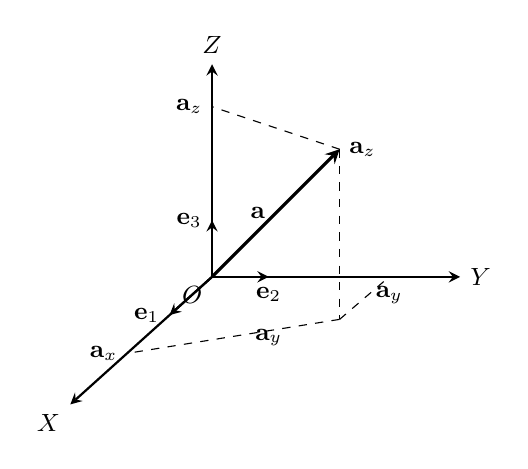
\begin{tikzpicture}[>=stealth, scale=0.9, font=\small]
  \draw[->, thick] (0, 0) -- (-2, -1.8) node[below left] {$X$};
  \draw[->, thick] (0, 0) -- (3.5, 0) node[right] {$Y$};
  \draw[->, thick] (0, 0) -- (0, 3) node[above] {$Z$};
  \node[below left] at (0, 0) {$O$};

  \coordinate (A) at (1.8, 1.8);
  \coordinate (Aprime) at (1.8, -0.6);

  \draw[->, very thick] (0, 0) -- (A) node[midway, left] {$\mathbf{a}$};
  \draw[->, thick] (0, 0) -- (-0.6, -0.54) node[left] {$\mathbf{e}_1$};
  \draw[->, thick] (0, 0) -- (0.8, 0) node[below] {$\mathbf{e}_2$};
  \draw[->, thick] (0, 0) -- (0, 0.8) node[left] {$\mathbf{e}_3$};

  \draw[dashed] (A) -- (Aprime);
  \draw[dashed] (Aprime) -- (-1.2, -1.08) node[left] {$\mathbf{a}_x$};
  \draw[dashed] (Aprime) -- (2.5, 0) node[below] {$\mathbf{a}_y$};
  \draw[dashed] (A) -- (0, 2.4) node[left] {$\mathbf{a}_z$};

  \node[right] at (A) {$\mathbf{a}_z$};
  \node[below] at (0.8, -0.6) {$\mathbf{a}_y$};
\end{tikzpicture}
\caption{空間向量之自然分解}
\label{fig:b3-fig3-34-1}
\end{minipage}
\hfill
\begin{minipage}{0.48\textwidth}
\centering
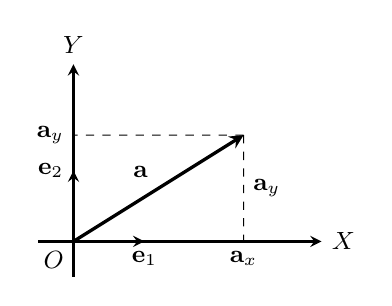
\begin{tikzpicture}[>=stealth, scale=0.9, font=\small]
  \draw[->, thick] (-0.5, 0) -- (3.5, 0) node[right] {$X$};
  \draw[->, thick] (0, -0.5) -- (0, 2.5) node[above] {$Y$};
  \node[below left] at (0, 0) {$O$};

  \coordinate (A) at (2.4, 1.5);
  \draw[->, very thick] (0, 0) -- (A) node[midway, above left] {$\mathbf{a}$};

  \draw[->, thick] (0, 0) -- (1, 0) node[below] {$\mathbf{e}_1$};
  \draw[->, thick] (0, 0) -- (0, 1) node[left] {$\mathbf{e}_2$};

  \draw[dashed] (A) -- (2.4, 0) node[below] {$\mathbf{a}_x$};
  \draw[dashed] (A) -- (0, 1.5) node[left] {$\mathbf{a}_y$};
  \node[right] at (2.4, 0.75) {$\mathbf{a}_y$};
\end{tikzpicture}
\caption{平面向量之自然分解}
\label{fig:b3-fig3-34-2}
\end{minipage}
\end{figure}

這樣的表示稱為向量 $\mathbf{a}$ 的一個自然分解.

同理，在平面上向量 $\mathbf{a}$ 的座標為 $(x, y)$ 的意思便是
\[ \mathbf{a} = x\mathbf{e}_1 + y\mathbf{e}_2. \]

現在來看看單位向量 $\mathbf{u}$ 的座標（或自然分解）：
\begin{proposition}
空間中任一單位向量 $\mathbf{u}$ 皆可表為
\[ \mathbf{u} = (\cos\alpha, \cos\beta, \cos\gamma), \]
其中 $\alpha, \beta, \gamma$ 分別是 $\mathbf{u}$ 與 $OX, OY, OZ$ 間的夾角角度.

這裏的 $\alpha, \beta$ 與 $\gamma$ 稱為 $\mathbf{u}$ 的方向角，而 $\cos\alpha, \cos\beta$ 與 $\cos\gamma$ 三個分量稱為 $\mathbf{u}$ 的方向餘弦.
\end{proposition}

\begin{proof}
設 $u_x, u_y, u_z$ 分別為 $\mathbf{u}$ 在 $\mathbf{e}_1, \mathbf{e}_2, \mathbf{e}_3$ 三方向上的投影，則因各投影量分別為 $|\mathbf{u}|\cos\alpha, |\mathbf{u}|\cos\beta, |\mathbf{u}|\cos\gamma$，而 $|\mathbf{u}| = 1$，故
\[ u_x = (\cos\alpha)\mathbf{e}_1, \quad u_y = (\cos\beta)\mathbf{e}_2, \quad u_z = (\cos\gamma)\mathbf{e}_3 \]
其中 $\alpha, \beta, \gamma$ 分別為 $\mathbf{u}$ 與 $u_x, u_y, u_z$ 間的夾角角度（$\alpha, \beta, \gamma$ 皆在 $0$ 與 $\pi$ 之間）. 因此
\begin{align*}
\mathbf{u} &= u_x + u_y + u_z \\
&= \cos\alpha\,\mathbf{e}_1 + \cos\beta\,\mathbf{e}_2 + \cos\gamma\,\mathbf{e}_3,
\end{align*}
即
\[ \mathbf{u} = (\cos\alpha, \cos\beta, \cos\gamma). \qedhere \]
\end{proof}

\begin{figure}[H]
\centering
\begin{tikzpicture}[>=stealth, scale=0.95, font=\small]
  \draw[->, thick] (0, 0) -- (-2, -1.8) node[below left] {$X$};
  \draw[->, thick] (0, 0) -- (3.5, 0) node[right] {$Y$};
  \draw[->, thick] (0, 0) -- (0, 3) node[above] {$Z$};
  \node[above left] at (0, 0) {$O$};

  \coordinate (U) at (1.5, 1.8);
  \draw[->, very thick] (0, 0) -- (U) node[above right] {$\mathbf{u}$};

  \draw[->, thick] (0, 0) -- (-0.6, -0.54) node[left] {$\mathbf{e}_1$};
  \draw[->, thick] (0, 0) -- (0.8, 0) node[below] {$\mathbf{e}_2$};
  \draw[->, thick] (0, 0) -- (0, 0.8) node[left] {$\mathbf{e}_3$};

  % Angles alpha, beta, gamma
  \node at (0.3, 1.2) {$\gamma$};
  \node at (0.8, 0.5) {$\beta$};
  \node at (-0.2, -0.3) {$\alpha$};

  \draw[dashed] (U) -- (1.5, -0.5);
  \draw[dashed] (1.5, -0.5) -- (-0.8, -0.72);
  \draw[dashed] (1.5, -0.5) -- (2.3, 0);
  \draw[dashed] (U) -- (0, 2.3);
\end{tikzpicture}
\caption{單位向量之方向角與方向餘弦}
\label{fig:b3-fig3-34-3}
\end{figure}

平面的情形只是特案，不妨另敘如下：
\begin{proposition*}[命題 $2'$]
平面上任一單位向量 $\mathbf{u}$ 皆可表為
\[ \mathbf{u} = (\cos\alpha, \cos\beta) \]
其中 $\alpha, \beta$ 分別是 $\mathbf{u}$ 與 $OX, OY$ 間的夾角角度. 其實在平面上我們常用來描寫方向的倒是所謂``矢角''的正餘弦，而不偏用餘弦.
\end{proposition*}

\begin{definition}
平面上一個向量 $\mathbf{a} = \vec{OA}$ 的矢角是射線 $\vec{OX}$ 繞到 $\vec{OA}$ 位置的（廣義）有向角的角度. 這個角度不特定取為某一個值，任何相差 $2n\pi$ 的角度都可作為同一向量的矢角. 例如下圖中
\[ \frac{\pi}{3}, \ -\frac{5\pi}{3}, \ \frac{7\pi}{3}, \ \dots\dots \text{皆為 } \mathbf{a} \text{ 的矢角}. \]
\end{definition}

現在命題 $2'$ 可改述如下：
設 $\omega$ 為平面上單位向量 $\mathbf{u}$ 的一個矢角，則因
\begin{align*}
\cos\omega &= \cos\alpha, \\
\sin\omega &= \sin\left(\frac{\pi}{2} - \beta\right) = \cos\beta
\end{align*}
故得
\[ \mathbf{u} = (\cos\omega, \sin\omega). \]

\begin{figure}[H]
\centering
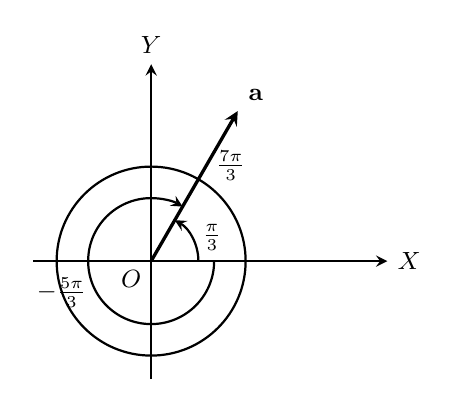
\begin{tikzpicture}[>=stealth, scale=1.0, font=\small]
  \draw[->, thick] (-1.5, 0) -- (3, 0) node[right] {$X$};
  \draw[->, thick] (0, -1.5) -- (0, 2.5) node[above] {$Y$};
  \node[below left] at (0, 0) {$O$};

  \coordinate (A) at (60:2.2);
  \draw[->, very thick] (0, 0) -- (A) node[above right] {$\mathbf{a}$};

  \draw[thick] (0, 0) circle (1.2cm);
  \draw[->, thick] (0.6, 0) arc (0:60:0.6) node[midway, right] {$\frac{\pi}{3}$};
  \draw[->, thick] (0.8, 0) arc (0:-300:0.8) node[midway, left] {$-\frac{5\pi}{3}$};

  \node[right] at (60:1.4) {$\frac{7\pi}{3}$};
\end{tikzpicture}
\caption{平面向量之矢角}
\label{fig:b3-fig3-35}
\end{figure}

\phantomsection\label{note:b3-ch3-p109-tau-typo}%
〔註〕矢角不限制在任何一段區域是為了實際的方便. 另一方面，由於考慮矢角時常考慮的是矢角的三角函數，故相差 $2n\pi$\footnote{【校訂註】原書末行註印作「故相差 $2n\tau$ 不致發生問題」，「$\tau$」實為「$\pi$」之殘字印刷訛誤。正文照原書字樣錄入並在此校記。} 不致發生問題.

\subsubsection*{乙、內積}

內積是用來考慮投影的，我們定義一個向量 $\mathbf{a}$ 與一單位向量 $\mathbf{u}$ 的內積為：$\mathbf{a}$ 在方向 $\mathbf{u}$ 上的投影量 $|\mathbf{a}|\cos\theta$，亦即
\begin{definition}
$\mathbf{a}\cdot\mathbf{u} = |\mathbf{a}|\cos\theta$，其中 $\theta$ 為 $\mathbf{a}$ 與 $\mathbf{u}$ 間的夾角角度，$\mathbf{u}$ 為單位向量.
\end{definition}

\begin{figure}[H]
\centering
\begin{minipage}{0.48\textwidth}
\centering
\begin{tikzpicture}[>=stealth, scale=0.9, font=\small]
  \coordinate (O) at (0, 0);
  \coordinate (A) at (0.4, 2.2);
  \coordinate (U) at (1.8, 1.2);

  \draw[->, very thick] (O) -- (A) node[midway, left] {$\mathbf{a}$};
  \draw[->, very thick] (O) -- (U) node[midway, below] {$\mathbf{u}$};

  \coordinate (P) at ($(O)!(A)!(U)$);
  \draw[dashed] (A) -- (P);
  \draw[thick] (O) -- (P) node[midway, below right] {$|\mathbf{a}|\cos\theta$};

  \draw[->] (0.4, 0.27) arc (33:78:0.4) node[midway, above] {$\theta$};
  \node[below left] at (O) {$O$};
\end{tikzpicture}
\caption*{此時投影量 $|\mathbf{a}|\cos\theta > 0$，即 $\mathbf{a}\cdot\mathbf{u} > 0$}
\caption{內積為正值}
\label{fig:b3-fig3-36-1}
\end{minipage}
\hfill
\begin{minipage}{0.48\textwidth}
\centering
\begin{tikzpicture}[>=stealth, scale=0.9, font=\small]
  \coordinate (O) at (0, 0);
  \coordinate (A) at (-1.5, 1.5);
  \coordinate (U) at (1.8, 0.8);

  \draw[->, very thick] (O) -- (A) node[midway, left] {$\mathbf{a}$};
  \draw[->, very thick] (O) -- (U) node[midway, below] {$\mathbf{u}$};

  \coordinate (P) at ($(O)!(A)!(U)$);
  \draw[dashed] (O) -- (P);
  \draw[dashed] (A) -- (P);
  \draw[thick] (O) -- (P) node[midway, below right] {$|\mathbf{a}|\cos\theta$};

  \draw[->] (0.4, 0.18) arc (24:135:0.4) node[midway, above] {$\theta$};
  \node[below] at (O) {$O$};
\end{tikzpicture}
\caption*{此時投影量 $|\mathbf{a}|\cos\theta < 0$，即 $\mathbf{a}\cdot\mathbf{u} < 0$}
\caption{內積為負值}
\label{fig:b3-fig3-36-2}
\end{minipage}
\end{figure}

\textbf{注意}：給了一向量 $\mathbf{a}$，要找在 $\mathbf{a}$ 本身方向的單位向量，只須將 $\mathbf{a}$ 除以 $\mathbf{a}$ 本身的長度 $|\mathbf{a}|$，此因 $\frac{\mathbf{a}}{|\mathbf{a}|}$ 變成了單位長：
\[ \left|\frac{\mathbf{a}}{|\mathbf{a}|}\right| = \left|\frac{1}{|\mathbf{a}|}\mathbf{a}\right| = \frac{1}{|\mathbf{a}|}|\mathbf{a}| = 1, \]
而方向仍然不變.

\begin{proposition}
設 $\mathbf{a}$ 為任給一向量，而 $\mathbf{u}_\mathbf{a}$ 為與 $\mathbf{a}$ 同向的單位向量，則 $\mathbf{a}$ 與 $\mathbf{u}_\mathbf{a}$ 的內積便是 $\mathbf{a}$ 的長度，即
\[ \mathbf{a}\cdot\mathbf{u}_\mathbf{a} = |\mathbf{a}|\cos 0 = |\mathbf{a}|. \qedhere \]
\end{proposition}

現在定義任意兩個一般向量的內積.
\begin{definition}
設 $\mathbf{a}, \mathbf{b}$ 為任意兩向量，定義
\[ \mathbf{a}\cdot\mathbf{b} = |\mathbf{a}||\mathbf{b}|\cos\theta \]
其中 $\theta$ 為 $\mathbf{b}$ 與 $\mathbf{a}$ 的夾角.（當 $\mathbf{a}$ 與 $\mathbf{b}$ 中有一為 $\mathbf{0}$ 時，定義 $\mathbf{a}\cdot\mathbf{b} = 0$）
\end{definition}

\textbf{注意}：向量的內積是一個實數，不是向量.
我們將內積的基本性質討論於下：

\textbf{內積性質 I}（交換性或對稱性）
\[ \mathbf{a}\cdot\mathbf{b} = \mathbf{b}\cdot\mathbf{a} \]
此因內積的定義 $\mathbf{a}\cdot\mathbf{b} = |\mathbf{a}||\mathbf{b}|\cos\theta = |\mathbf{b}||\mathbf{a}|\cos\theta = \mathbf{b}\cdot\mathbf{a}$.

\textbf{內積性質 II}
$\mathbf{a}$ 垂直於 $\mathbf{b}$（以後記成 $\mathbf{a} \perp \mathbf{b}$）的充分必要條件是
\[ \mathbf{a}\cdot\mathbf{b} = 0 \]
（$\mathbf{a}$ 與 $\mathbf{b}$ 有一為 $\mathbf{0}$ 時，不妨看成相互垂直.）

\begin{proof}
設 $\mathbf{a}$ 與 $\mathbf{b}$ 有一為 $\mathbf{0}$，由定義 $\mathbf{a}\cdot\mathbf{b} = 0$，故只須看 $\mathbf{a}$ 與 $\mathbf{b}$ 全不為 $\mathbf{0}$ 的場合，此時
\[ \mathbf{a}\cdot\mathbf{b} = |\mathbf{a}||\mathbf{b}|\cos\theta \]
故 $\mathbf{a}\cdot\mathbf{b} = 0$ 的充分必要條件是 $\cos\theta = 0$，亦即 $\theta = \frac{\pi}{2}$，即 $\mathbf{a}$ 垂直於 $\mathbf{b}$. \qedhere
\end{proof}

\begin{figure}[H]
\centering
\begin{tikzpicture}[>=stealth, scale=0.9, font=\small]
  \coordinate (O) at (0, 0);
  \coordinate (A) at (40:2);
  \coordinate (B) at (130:1.8);

  \draw[->, very thick] (O) -- (A) node[midway, below right] {$\mathbf{a}$};
  \draw[->, very thick] (O) -- (B) node[midway, below left] {$\mathbf{b}$};
  \draw (0.3, 0) arc (0:90:0.3);
  \node at (0.1, 0.45) {\scriptsize $\frac{\pi}{2}$};
  \node[below] at (0, -0.2) {此時 $\mathbf{a}\cdot\mathbf{b} = 0$};
\end{tikzpicture}
\caption{相互垂直向量之內積為零}
\label{fig:b3-fig3-37}
\end{figure}

\begin{proposition}
$\mathbf{a}\cdot\mathbf{a} = |\mathbf{a}||\mathbf{a}|\cos 0 = |\mathbf{a}|^2$.
即 $\mathbf{a}$ 與 $\mathbf{a}$ 自己的內積就是 $\mathbf{a}$ 的長度的平方. \qedhere
\end{proposition}

\textbf{內積性質 III}（正定性）：
若 $\mathbf{a} \ne \mathbf{0}$，則 $\mathbf{a}\cdot\mathbf{a} = |\mathbf{a}|^2 > 0$.

\textbf{內積性質 IV}：
\[ \mathbf{a}\cdot(\alpha\mathbf{b}) = (\alpha\mathbf{a})\cdot\mathbf{b} = \alpha(\mathbf{a}\cdot\mathbf{b}). \]
證明 留做習題.

\subsubsection*{丙、內積的座標成分表示}

我們依賴幾何的定義引入的內積，若不能給它一個代數的座標表示，它只是一個人為的空洞的東西，於實際問題的處理是無益的. 譬如，空間給定兩個向量 $\mathbf{a}$ 與 $\mathbf{b}$ 的夾角 $\theta$ 一般時候是難以求得，因此 $\mathbf{a}\cdot\mathbf{b} = |\mathbf{a}||\mathbf{b}|\cos\theta$ 式子究其實是無助於任何計算的，它只是一個幾何的定義.

幸好下面的定理 4（內積的代數表示）可成功地設立：

\begin{theorem}
設 $\mathbf{a} = (x_1, y_1, z_1), \mathbf{b} = (x_2, y_2, z_2)$，則
\[ \mathbf{a}\cdot\mathbf{b} = x_1 x_2 + y_1 y_2 + z_1 z_2. \]
\end{theorem}
（這是一個重要的代數表示，我們將看到藉著這易於計算的代數表示，內積會發揮很大的作用.）

\begin{proof}[證明（用餘弦定律）]
取 $A, B$ 兩點，使 $\mathbf{a} = \vec{OA}, \mathbf{b} = \vec{OB}$. 則 $\mathbf{a}, \mathbf{b}$ 及 $\mathbf{a} - \mathbf{b}$ 可圍成一三角形 $OAB$，如圖：

\begin{figure}[H]
\centering
\begin{minipage}{0.48\textwidth}
\centering
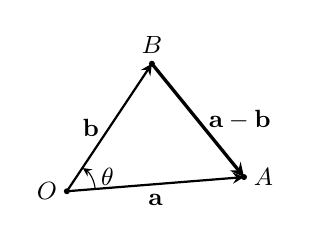
\begin{tikzpicture}[>=stealth, scale=0.9, font=\small]
  \coordinate (O) at (0, 0);
  \coordinate (A) at (2.5, 0.2);
  \coordinate (B) at (1.2, 1.8);

  \draw[->, thick] (O) -- (A) node[midway, below] {$\mathbf{a}$};
  \draw[->, thick] (O) -- (B) node[midway, left] {$\mathbf{b}$};
  \draw[->, very thick] (B) -- (A) node[midway, right] {$\mathbf{a}-\mathbf{b}$};
  \draw[->] (0.4, 0.03) arc (5:56:0.4) node[midway, right] {$\theta$};

  \fill (O) circle (1.2pt) node[left] {$O$};
  \fill (A) circle (1.2pt) node[right] {$A$};
  \fill (B) circle (1.2pt) node[above] {$B$};
\end{tikzpicture}
\caption{銳角情形}
\label{fig:b3-fig3-38-1}
\end{minipage}
\hfill
\begin{minipage}{0.48\textwidth}
\centering
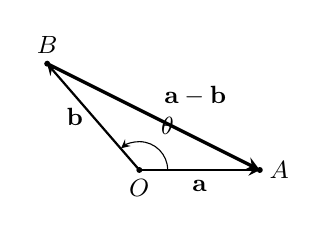
\begin{tikzpicture}[>=stealth, scale=0.9, font=\small]
  \coordinate (O) at (1.5, 0);
  \coordinate (A) at (3.2, 0);
  \coordinate (B) at (0.2, 1.5);

  \draw[->, thick] (O) -- (A) node[midway, below] {$\mathbf{a}$};
  \draw[->, thick] (O) -- (B) node[midway, left] {$\mathbf{b}$};
  \draw[->, very thick] (B) -- (A) node[midway, above right] {$\mathbf{a}-\mathbf{b}$};
  \draw[->] (1.9, 0) arc (0:130:0.4) node[midway, above right] {$\theta$};

  \fill (O) circle (1.2pt) node[below] {$O$};
  \fill (A) circle (1.2pt) node[right] {$A$};
  \fill (B) circle (1.2pt) node[above] {$B$};
\end{tikzpicture}
\caption{鈍角情形}
\label{fig:b3-fig3-38-2}
\end{minipage}
\end{figure}

由餘弦定律：
\begin{align*}
|\mathbf{a} - \mathbf{b}|^2 &= |\mathbf{a}|^2 + |\mathbf{b}|^2 - 2|\mathbf{a}||\mathbf{b}|\cos\theta \\
&= |\mathbf{a}|^2 + |\mathbf{b}|^2 - 2\mathbf{a}\cdot\mathbf{b} \\
-2\mathbf{a}\cdot\mathbf{b} &= |\mathbf{a} - \mathbf{b}|^2 - |\mathbf{a}|^2 - |\mathbf{b}|^2 \\
&= (x_1 - x_2)^2 + (y_1 - y_2)^2 + (z_1 - z_2)^2 \\
&\quad - (x_1^2 + y_1^2 + z_1^2) - (x_2^2 + y_2^2 + z_2^2) \\
&= -(2x_1 x_2 + 2y_1 y_2 + 2z_1 z_2)
\end{align*}
故
\[ \mathbf{a}\cdot\mathbf{b} = x_1 x_2 + y_1 y_2 + z_1 z_2. \]
這個代數表示顯示出 $\mathbf{a}\cdot\mathbf{b}$ 能簡潔地用各相應成分乘積的總和來計算. \qedhere
\end{proof}

\textbf{注意}：當 $\mathbf{a}$ 與 $\mathbf{b}$ 為平面上的向量時，設 $\mathbf{a} = (x_1, y_1), \mathbf{b} = (x_2, y_2)$，則 $\mathbf{a}\cdot\mathbf{b} = x_1 x_2 + y_1 y_2$. 它的道理將留當作業.

\begin{example}[論例 9]
求空間中兩向量 $\mathbf{a} = \vec{OA} = (x_1, y_1, z_1), \mathbf{b} = \vec{OB} = (x_2, y_2, z_2)$ 的夾角 $\theta$.
\end{example}

\begin{figure}[H]
\centering
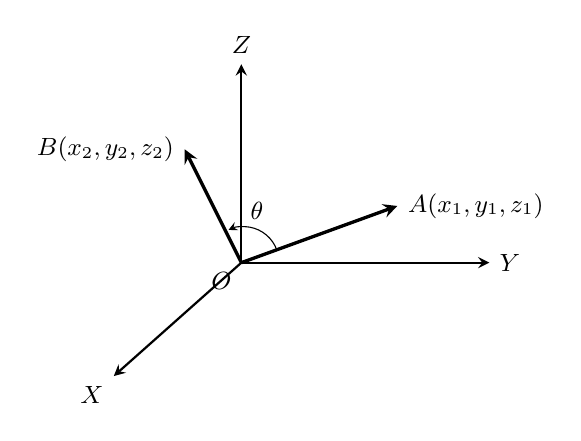
\begin{tikzpicture}[>=stealth, scale=0.9, font=\small]
  \draw[->, thick] (0, 0) -- (-1.8, -1.6) node[below left] {$X$};
  \draw[->, thick] (0, 0) -- (3.5, 0) node[right] {$Y$};
  \draw[->, thick] (0, 0) -- (0, 2.8) node[above] {$Z$};
  \node[below left] at (0, 0) {$O$};

  \coordinate (A) at (2.2, 0.8);
  \coordinate (B) at (-0.8, 1.6);

  \draw[->, very thick] (0, 0) -- (A) node[right] {$A(x_1, y_1, z_1)$};
  \draw[->, very thick] (0, 0) -- (B) node[left] {$B(x_2, y_2, z_2)$};

  \draw[->] (0.5, 0.18) arc (20:115:0.5) node[midway, above] {$\theta$};
\end{tikzpicture}
\caption{空間兩向量夾角}
\label{fig:b3-fig3-39}
\end{figure}

\begin{proof}[解]
\phantomsection\label{note:b3-ch3-p113-cos-theta-typo}%
由定義
\[ \mathbf{a}\cdot\mathbf{b} = |\mathbf{a}||\mathbf{b}|\cos\theta\footnote{【校訂註】原書頁 113 末行解文印作「$\mathbf{a}\cdot\mathbf{b} = |\mathbf{a}||\mathbf{b}|\cos v$」，「$v$」實為夾角符號「$\theta$」之字模排印訛字。正文照原書字樣錄入並在此校記。} \]
但 $\mathbf{a}\cdot\mathbf{b} = x_1 x_2 + y_1 y_2 + z_1 z_2$，故
\[ \cos\theta = \frac{\mathbf{a}\cdot\mathbf{b}}{|\mathbf{a}||\mathbf{b}|} = \frac{x_1 x_2 + y_1 y_2 + z_1 z_2}{\sqrt{x_1^2 + y_1^2 + z_1^2}\sqrt{x_2^2 + y_2^2 + z_2^2}}. \qedhere \]
\end{proof}

最後這個式子很有用，但不必去死背，每次要用它，只要回想內積的幾何意義（本解第一式）及其代數表示（本解第二式），作一比較即得.

\begin{example}
一正立方體兩對角線相交，其兩交角若干？
\end{example}

\begin{figure}[H]
\centering
\begin{tikzpicture}[>=stealth, scale=1.0, font=\small]
  \draw[->, thick] (0, 0) -- (-1.8, -1.6) node[below left] {$X$};
  \draw[->, thick] (0, 0) -- (3.2, 0) node[right] {$Y$};
  \draw[->, thick] (0, 0) -- (0, 2.8) node[above] {$Z$};
  \node[below left] at (0, 0) {$O$};

  % Cube vertices
  \coordinate (O) at (0, 0);
  \coordinate (P1) at (-0.8, -0.72); % (1, 0, 0)
  \coordinate (P2) at (1.8, 0);      % (0, 1, 0)
  \coordinate (P3) at (0, 1.8);      % (0, 0, 1)
  \coordinate (P12) at ($(P1) + (P2)$); % (1, 1, 0)
  \coordinate (P13) at ($(P1) + (P3)$); % (1, 0, 1)
  \coordinate (P23) at ($(P2) + (P3)$); % (0, 1, 1)
  \coordinate (P) at ($(P12) + (P3)$);  % (1, 1, 1)

  % Cube edges
  \draw[thick] (P1) -- (P12) -- (P2);
  \draw[thick] (P3) -- (P13) -- (P) -- (P23) -- cycle;
  \draw[thick] (P1) -- (P13);
  \draw[thick] (P12) -- (P);
  \draw[thick] (P2) -- (P23);

  % Diagonals
  \draw[very thick] (0, 0) -- (P);
  \draw[dashed, very thick] (P3) -- (P12);

  \fill (P3) circle (1.2pt) node[left] {$P_3(0, 0, 1)$};
  \fill (P) circle (1.2pt) node[right] {$P(1, 1, 1)$};
  \fill (P12) circle (1.2pt) node[below] {$P'(1, 1, 0)$};
  \fill (P13) circle (1.2pt) node[left] {$(1, 0, 1)$};
  \fill (P23) circle (1.2pt) node[above right] {$(0, 1, 1)$};
  \fill (P1) circle (1.2pt) node[below left] {$(1, 0, 0)$};
  \fill (P2) circle (1.2pt) node[below] {$(0, 1, 0)$};
\end{tikzpicture}
\caption{正立方體對角線夾角}
\label{fig:b3-fig3-40}
\end{figure}

\begin{proof}[解]
取座標系 $(O; X, Y, Z)$ 使正立方體座標落如圖，因這正立方體的大小不影響對角線交角，故可設其邊長為 1 以便計算：設
\begin{align*}
\mathbf{a} &= \vec{OP} = (1, 1, 1) \\
\mathbf{b} &= \vec{P_3 P'} = (1, 1, 0) - (0, 0, 1) = (1, 1, -1)
\end{align*}
故
\[ \mathbf{a}\cdot\mathbf{b} = (1, 1, 1)\cdot(1, 1, -1) = 1 + 1 - 1 = 1 \]
而 $\mathbf{a}\cdot\mathbf{b} = |\mathbf{a}||\mathbf{b}|\cos\theta$. 其中
\begin{align*}
|\mathbf{a}| &= \sqrt{1^2 + 1^2 + 1^2} = \sqrt{3} \\
|\mathbf{b}| &= \sqrt{1^2 + 1^2 + (-1)^2} = \sqrt{3}
\end{align*}
因此，$\mathbf{a}\cdot\mathbf{b}$ 的代數表示與幾何定義一經比較得
\[ 1 = \mathbf{a}\cdot\mathbf{b} = \sqrt{3}\sqrt{3}\cos\theta \]
故
\[ \cos\theta = \frac{1}{3} \]
查三角函數表得 $\theta = 70^\circ 32'$.
另一交角為 $180^\circ - 70^\circ 32' = 109^\circ 28'$. \qedhere
\end{proof}

我們已談過 $\mathbf{a} \perp \mathbf{b} \iff \mathbf{a}\cdot\mathbf{b} = 0$，現在從 $\mathbf{a}\cdot\mathbf{b} = x_1 x_2 + y_1 y_2 + z_1 z_2$ 立即考得：

\begin{proposition}
空間中的兩向量 $\mathbf{a} = (x_1, y_1, z_1), \mathbf{b} = (x_2, y_2, z_2)$ 相互垂直的充要條件是 $\mathbf{a}\cdot\mathbf{b} = 0$，亦即
\[ x_1 x_2 + y_1 y_2 + z_1 z_2 = 0 \]
當 $\mathbf{a} = (x_1, y_1), \mathbf{b} = (x_2, y_2)$ 為平面上的向量時，則 $\mathbf{a} \perp \mathbf{b}$ 的充要條件是
\[ x_1 x_2 + y_1 y_2 = 0 \]
或存在一實數 $k$ 使得 $x_1 = k y_2, y_1 = -k x_2$.
\end{proposition}
〔註〕$\mathbf{a}$ 或 $\mathbf{b}$ 有一為零向量時亦視 $\mathbf{a}$ 與 $\mathbf{b}$ 垂直.

\subsubsection*{作業 7}
\begin{enumerate}[label=(\roman*), leftmargin=2em]
  \item 設 $\mathbf{a} = (2, 4), \mathbf{b} = (10, -5)$，試證 $\mathbf{a} \perp \mathbf{b}$.
  \item 設 $\mathbf{a} = (-1, 2, -1), \mathbf{b} = (1, 2, 3)$，問 $\mathbf{a}, \mathbf{b}$ 是否相互垂直？
  \item 設 $\mathbf{a} = (-3, 4), \mathbf{b} = (2, 1)$，求在 $\mathbf{b}$ 的方向上的單位向量 $\mathbf{u}$，並求 $\mathbf{a}$ 在 $\mathbf{u}$ 方向上的投影量. 又在方格紙上繪圖，以查驗你的結果是否與圖上的大略相符.
\end{enumerate}

\begin{example}
利用內積求證內接於一半圓的角必為直角，即右圖中，$C$ 為半圓弧 $\wideparen{AB}$ 上任一點，則 $\angle ACB$ 為直角.
\end{example}

\begin{figure}[H]
\centering
\begin{tikzpicture}[>=stealth, scale=0.95, font=\small]
  \draw[->, thick] (-2.5, 0) -- (2.5, 0) node[right] {$X$};
  \draw[->, thick] (0, -0.5) -- (0, 2.2) node[above] {$Y$};
  \node[below left] at (0, 0) {$O$};

  \draw[thick] (1.8, 0) arc (0:180:1.8);
  \coordinate (A) at (1.8, 0);
  \coordinate (B) at (-1.8, 0);
  \coordinate (C) at (45:1.8);

  \draw[thick] (A) -- (C) -- (B);
  \draw[dashed] (0, 0) -- (C) node[midway, left] {$r$};

  \fill (A) circle (1.5pt) node[below] {$A(r, 0)$};
  \fill (B) circle (1.5pt) node[below] {$B(-r, 0)$};
  \fill (C) circle (1.5pt) node[above right] {$C(x, y)$};
  \node[below] at (0.9, 0) {$r$};
\end{tikzpicture}
\caption{半圓內接角為直角}
\label{fig:b3-fig3-41}
\end{figure}

\begin{proof}
取直角座標系 $(O; X, Y)$ 使 $O$ 為圓心，$\vec{AB}$ 在 $X$ 軸上，設半徑為 $r$，則 $A, B$ 座標為
\[ A(r, 0), \quad B(-r, 0) \]
設 $C$ 之座標為 $C(x, y)$，則
\[ \vec{AC} = (x - r, y), \quad \vec{BC} = (x + r, y), \]
得
\[ \vec{AC}\cdot\vec{BC} = (x - r)(x + r) + y^2 = x^2 - r^2 + y^2 \]
但 $C$ 在該半圓上，
\[ r^2 = \overline{OC}^2 = x^2 + y^2 \]
\phantomsection\label{note:b3-ch3-p116-ac-bc-zero}%
故 $\vec{AC}\cdot\vec{BC} = x^2 + y^2 - r^2 = 0$\footnote{【校訂註】原書排印作「$x^2+y^2-r^2 = C$ 即 $\vec{AC}\perp\vec{BC}$」，等號右端「$C$」顯為數字「$0$」之印刷訛字。正文照原書字樣錄入並在此校記。} 即 $\vec{AC} \perp \vec{BC}$. \qedhere
\end{proof}

\subsubsection*{丁、內積的分配律}

內積的分配律不難由其幾何定義證明，但利用其代數表示更直截.

\textbf{內積性質 V}（分配律）
\[ \mathbf{a}\cdot(\mathbf{b} + \mathbf{c}) = \mathbf{a}\cdot\mathbf{b} + \mathbf{a}\cdot\mathbf{c} \]
（它的成立是基於內積的代數表示中已顯示問題能歸結於實數系中的分配律.）

\begin{figure}[H]
\centering
\begin{tikzpicture}[>=stealth, scale=0.9, font=\small]
  \coordinate (O) at (0, 0);
  \coordinate (A) at (3.5, 0);
  \coordinate (B) at (1.5, 0.8);
  \coordinate (C) at (1.8, 2.5);

  \draw[->, very thick] (O) -- (A) node[right] {$\mathbf{a}$};
  \draw[->, thick] (O) -- (B) node[midway, above left] {$\mathbf{b}$};
  \draw[->, thick] (B) -- (C) node[midway, right] {$\mathbf{c}$};
  \draw[->, very thick] (O) -- (C) node[midway, left] {$\mathbf{b}+\mathbf{c}$};

  % Projections on a
  \draw[dashed] (B) -- (1.5, 0);
  \draw[dashed] (C) -- (1.8, 0);

  \node[above] at (C) {$\mathbf{c}$};
\end{tikzpicture}
\caption{內積分配律之幾何投影}
\label{fig:b3-fig3-42}
\end{figure}

\begin{proof}
設 $\mathbf{a} = (x_1, y_1, z_1), \mathbf{b} = (x_2, y_2, z_2), \mathbf{c} = (x_3, y_3, z_3)$
\begin{align*}
\mathbf{a}\cdot(\mathbf{b} + \mathbf{c}) &= x_1(x_2 + x_3) + y_1(y_2 + y_3) + z_1(z_2 + z_3) \\
&= x_1 x_2 + x_1 x_3 + y_1 y_2 + y_1 y_3 + z_1 z_2 + z_1 z_3 \\
&= (x_1 x_2 + y_1 y_2 + z_1 z_2) + (x_1 x_3 + y_1 y_3 + z_1 z_3) \\
&= \mathbf{a}\cdot\mathbf{b} + \mathbf{a}\cdot\mathbf{c}. \qedhere
\end{align*}
\end{proof}

至於幾何的證明，則可如圖 3-36 從射影量來說，同學可繪圖（如圖 3-42）證之.

\subsubsection*{戊、向量處理的例子}

我們以著名且常用的舒瓦茲（Schwartz）不等式，結束這節的討論.

\begin{theorem}[舒瓦茲不等式 Schwartz Inequality]
對任意實數 $x_1, y_1, z_1, x_2, y_2, z_2$，不等式
\[ (x_1 x_2 + y_1 y_2 + z_1 z_2)^2 \le (x_1^2 + y_1^2 + z_1^2)(x_2^2 + y_2^2 + z_2^2) \]
永遠成立，表成向量記號，則為
\[ |\mathbf{a}\cdot\mathbf{b}|^2 \le |\mathbf{a}|^2|\mathbf{b}|^2 \]
其中 $\mathbf{a} = (x_1, y_1, z_1), \mathbf{b} = (x_2, y_2, z_2)$.
\end{theorem}

\begin{proof}
這定理的關鍵在於利用內積幾何定義與其代數表示的一致性：
\begin{align*}
(x_1 x_2 + y_1 y_2 + z_1 z_2)^2 &= |\mathbf{a}\cdot\mathbf{b}|^2 \quad \text{〔內積代數表示〕} \\
&= |\mathbf{a}|^2|\mathbf{b}|^2\cos^2\theta \quad \text{〔內積幾何定義〕} \\
&\le |\mathbf{a}|^2|\mathbf{b}|^2 \quad \text{〔}\cos^2\theta \le 1\text{〕} \\
&= (x_1^2 + y_1^2 + z_1^2)(x_2^2 + y_2^2 + z_2^2) \quad \text{〔長度 $|\mathbf{a}|$ 的成分表示〕}. \qedhere
\end{align*}
\end{proof}

\begin{example}[論例 10 （畢氏定理的向量表示式）]
空間中兩向量 $\mathbf{a}$ 與 $\mathbf{b}$ 相互垂直的充要條件為
\[ |\mathbf{a} + \mathbf{b}|^2 = |\mathbf{a}|^2 + |\mathbf{b}|^2 \]
\end{example}

\begin{figure}[H]
\centering
\begin{tikzpicture}[>=stealth, scale=0.9, font=\small]
  \coordinate (O) at (0, 0);
  \coordinate (A) at (2.5, 0);
  \coordinate (B) at (2.5, 1.8);

  \draw[->, very thick] (O) -- (A) node[midway, below] {$\mathbf{a}$};
  \draw[->, very thick] (A) -- (B) node[midway, right] {$\mathbf{b}$};
  \draw[->, very thick] (O) -- (B) node[midway, above left] {$\mathbf{a}+\mathbf{b}$};

  \draw (2.3, 0) -- (2.3, 0.2) -- (2.5, 0.2);
\end{tikzpicture}
\caption{畢氏定理之向量表示}
\label{fig:b3-fig3-43}
\end{figure}

\begin{proof}
\begin{align*}
|\mathbf{a} + \mathbf{b}|^2 &= (\mathbf{a} + \mathbf{b})\cdot(\mathbf{a} + \mathbf{b}) \\
&= (\mathbf{a} + \mathbf{b})\cdot\mathbf{a} + (\mathbf{a} + \mathbf{b})\cdot\mathbf{b} \quad \text{〔分配律〕} \\
&= \mathbf{a}\cdot\mathbf{a} + \mathbf{b}\cdot\mathbf{a} + \mathbf{a}\cdot\mathbf{b} + \mathbf{b}\cdot\mathbf{b} \quad \text{〔分配律〕} \\
&= |\mathbf{a}|^2 + 2\mathbf{a}\cdot\mathbf{b} + |\mathbf{b}|^2
\end{align*}
但 $\mathbf{a} \perp \mathbf{b}$ 的充要條件為 $\mathbf{a}\cdot\mathbf{b} = 0$，根據上式知其充要條件可寫成
\[ |\mathbf{a} + \mathbf{b}|^2 = |\mathbf{a}|^2 + |\mathbf{b}|^2. \qedhere \]
\end{proof}

\begin{example}[論例 11 （外心定理）]
$\Delta ABC$ 三邊 $BC, CA, AB$ 上三條垂直平分線 $L_1, L_2$ 與 $L_3$ 交會於一點.
\end{example}

\begin{figure}[H]
\centering
\begin{tikzpicture}[>=stealth, scale=0.9, font=\small]
  \coordinate (A) at (2.0, 3.0);
  \coordinate (B) at (0, 0.6);
  \coordinate (C) at (3.5, 0.6);

  \coordinate (D) at ($(B)!0.5!(C)$);
  \coordinate (E) at ($(C)!0.5!(A)$);
  \coordinate (F) at ($(A)!0.5!(B)$);

  % Circumcenter M
  \coordinate (M) at (1.75, 1.4);

  \draw[thick] (A) -- (B) -- (C) -- cycle;

  % Perpendicular bisectors
  \draw[thick] (D) -- ++(0, -0.6) node[right] {$L_1$};
  \draw[thick] (D) -- (M);
  \draw[thick] (E) -- ++(0.8, 0.3) node[above] {$L_2$};
  \draw[thick] (E) -- (M);
  \draw[thick] (F) -- (M);

  \fill (A) circle (1.2pt) node[above] {$A$};
  \fill (B) circle (1.2pt) node[left] {$B$};
  \fill (C) circle (1.2pt) node[right] {$C$};
  \fill (D) circle (1.2pt) node[below] {$D$};
  \fill (E) circle (1.2pt) node[right] {$E$};
  \fill (F) circle (1.2pt) node[left] {$F$};
  \fill (M) circle (1.5pt) node[right] {$M$};
\end{tikzpicture}
\caption{三角形外心定理}
\label{fig:b3-fig3-44}
\end{figure}

\begin{proof}
設 $D, E, F$ 分別為 $\overline{BC}, \overline{CA}, \overline{AB}$ 三邊中點. 設 $L_1$ 與 $L_2$ 交於 $M$，連結 $MF$，若證得 $MF \perp AB$，亦即
\[ \vec{MF}\cdot\vec{AB} = 0 \]
則本定理亦將得證. 以下我們逐步利用向量各種運算來一邊演繹一邊簡化 $\vec{MF}\cdot\vec{AB}$ 這一內積.

但這演繹與簡化的過程基於「儘量利用已知條件」這一原則. 故先重複一下已知條件：
\begin{enumerate}[label=(\roman*), leftmargin=2.5em]
  \item $L_1$ 為 $BC$ 邊上垂直平分線，即：$\vec{MD}\cdot\vec{BC} = 0$，且
  \[ \vec{MD} = \frac{1}{2}\vec{MB} + \frac{1}{2}\vec{MC}. \]
  \item $L_2$ 為 $CA$ 邊上垂直平分線，即：$\vec{ME}\cdot\vec{CA} = 0$，且
  \[ \vec{ME} = \frac{1}{2}\vec{MC} + \frac{1}{2}\vec{MA}. \]
  \item $F$ 為 $\overline{AB}$ 邊中點，即 $\vec{MF} = \frac{1}{2}\vec{MA} + \frac{1}{2}\vec{MB}$.
\end{enumerate}
\begin{align*}
\vec{MF}\cdot\vec{AB} &= \frac{1}{2}(\vec{MA} + \vec{MB})\cdot(\vec{MB} - \vec{MA}) \quad \text{〔因 (iii)〕} \\
&= \frac{1}{2}(\overline{MB}^2 - \overline{MA}^2)
\end{align*}
要證明 $\vec{MF}\cdot\vec{AB} = 0$，便須證明 $\overline{MB} = \overline{MA}$.

但想一下另兩邊上，亦有
\begin{align*}
0 &= \vec{MD}\cdot\vec{BC} = \frac{1}{2}(\vec{MB} + \vec{MC})\cdot(\vec{MC} - \vec{MB}) \quad \text{〔因 (i)〕} \\
&= \frac{1}{2}(\overline{MC}^2 - \overline{MB}^2) \\
0 &= \vec{ME}\cdot\vec{CA} = \frac{1}{2}(\vec{MC} + \vec{MA})\cdot(\vec{MA} - \vec{MC}) \quad \text{〔因 (ii)〕} \\
&= \frac{1}{2}(\overline{MA}^2 - \overline{MC}^2)
\end{align*}
故
\[ \overline{MB} = \overline{MC} = \overline{MA} \]
即 $\vec{MF}\cdot\vec{AB} = 0$，得知三個垂直平分線共點. \qedhere
\end{proof}

\subsubsection*{作業 8}
利用向量運算，求證三角形三個高交會於一點（垂心定理）.

\subsubsection*{習題 3-5}

\begin{enumerate}[label=\arabic*., leftmargin=2em]
  \item 設 $\mathbf{a} = \mathbf{e}_1 + 2\mathbf{e}_2 + 3\mathbf{e}_3$，試求 $\mathbf{a}$ 的長度及其方向上的單位向量.
  \item 設
  \begin{align*}
  \mathbf{a} &= 3\mathbf{e}_1 + 20\mathbf{e}_2 - 15\mathbf{e}_3 \\
  \mathbf{b} &= 2\mathbf{e}_1 + 5\mathbf{e}_3 \\
  \mathbf{c} &= 7\mathbf{e}_1 + 11\mathbf{e}_2 - 2\mathbf{e}_3
  \end{align*}
  試求 $\mathbf{a}\cdot\mathbf{b}, \mathbf{a}\cdot\mathbf{a}$ 及 $\mathbf{a}\cdot\mathbf{c} - \mathbf{b}\cdot\mathbf{c}$.
  \item 設平面上單位向量 $\mathbf{u}$ 與 $X$-軸之交角為 $\frac{\pi}{4}$（$\mathbf{u}$ 有兩種可能），試求 $\mathbf{u}$ 在 $X$-軸、$Y$-軸的成分.
  \item 設 $\mathbf{a} = 2\mathbf{e}_1 - 3\mathbf{e}_2, \mathbf{b} = 3\mathbf{e}_1 + 4\mathbf{e}_2$，試求 $\mathbf{a}$ 沿著 $\mathbf{b}$ 方向的投影量與投影.
  \item 設 $\mathbf{a} = 2\mathbf{e}_1 + 4\mathbf{e}_2 - 7\mathbf{e}_3, \mathbf{b} = 2\mathbf{e}_1 + 6\mathbf{e}_2 + x\mathbf{e}_3$，試求 $x$ 使得 $\mathbf{a} \perp \mathbf{b}$.
  \item 若 $|\mathbf{a} - \mathbf{b}| = |\mathbf{a}| + |\mathbf{b}|$，試求 $\mathbf{a}$ 與 $\mathbf{b}$ 的關係.
  \item 試證 若 $\mathbf{a}, \mathbf{b}$ 皆非零向量，則 $-1 \le \frac{\mathbf{a}\cdot\mathbf{b}}{|\mathbf{a}||\mathbf{b}|} \le 1$.
  \item 利用內積證明正方形之對角線互相垂直.
  \item 設 $ABCD$ 為一平行四邊形，利用向量證明 $\overline{AC}^2 + \overline{BD}^2 = 2(\overline{AB}^2 + \overline{AD}^2)$.
  \item 證明並圖解內積性質 IV: $\mathbf{a}\cdot(\alpha\mathbf{b}) = (\alpha\mathbf{a})\cdot\mathbf{b} = \alpha(\mathbf{a}\cdot\mathbf{b})$.
  \item 試用幾何圖形及投影量定義，證明內積分配律.
  \item 設 $P = (6, -4, 4), Q = (2, 1, 2), R = (3, -1, 4)$，求 $P$ 至 $\vec{QR}$ 之最短距離.
  \item 如 $\mathbf{a} = (4, -1, 3), \mathbf{b} = (-2, 1, -2)$，求一單位向量垂直 $\mathbf{a}$ 和 $\mathbf{b}$.
  \item 設一颱風中心 $O$，下午三時被測出在 $A$ 地南 $30^\circ$ 東方向，距 $A$ 地 100 公里的海面上，正朝北 $15^\circ$ 西的方向，以每時 24 公里速度侵襲，且其暴風半徑為 40 公里. 假定這颱風方向及進行速度不變，預測何時 $A$ 地會進入暴風圈內？何時可望脫離？
  \item
  \begin{enumerate}[label=(\roman*), leftmargin=2em]
    \item 設 $C(1, 1, 1), B(3, -6, 2), A(3, 1, 2), \mathbf{a} = \vec{BA}, \mathbf{c} = \vec{BC}$ 求 $\mathbf{a}\cdot\mathbf{c}$ 之值.
    \item 設在 $A, B, C$ 三點所張出之平面上一點 $P$，滿足 $\overline{PA} = \overline{PB}$. 且 $P$ 到直線 $AB$ 之距離為 2，求 $P$ 點之座標.\\
    〔提示：$P$ 應該在線段 $AB$ 之垂直平分線上，設 $M$ 為 $AB$ 中點，則
    \[ \vec{OP} = \vec{OA} + \vec{AM} + \vec{MP} = \vec{OA} + \frac{1}{2}(\vec{OB} - \vec{OA}) + 2\mathbf{u} \]
    其中 $\mathbf{u}$ 為該平面上垂直於 $AB$ 之一單位向量，所剩的便是如何利用 $\mathbf{a}\cdot\mathbf{c}$ 來求 $\mathbf{u}$〕
  \end{enumerate}
\end{enumerate}

\begin{figure}[H]
\centering
\begin{tikzpicture}[>=stealth, scale=0.9, font=\small]
  \coordinate (O) at (0, 0);
  \coordinate (A) at (0, 2.0);
  \coordinate (B) at (3.5, 1.2);
  \coordinate (C) at (2.0, 2.6);

  \coordinate (M) at ($(A)!0.5!(B)$);
  \coordinate (P) at ($(M) + (-0.5, 1.0)$);

  \draw[thick] (A) -- (B) node[midway, above] {$\mathbf{a}$};
  \draw[thick] (B) -- (C) node[midway, right] {$\mathbf{c}$};
  \draw[thick] (A) -- (C);

  \draw[dashed] (O) -- (A);
  \draw[dashed] (O) -- (B);
  \draw[dashed] (O) -- (C);
  \draw[dashed] (O) -- (M);
  \draw[very thick] (O) -- (P);
  \draw[thick] (M) -- (P);

  \fill (O) circle (1.2pt) node[below] {$O$};
  \fill (A) circle (1.2pt) node[above left] {$A$};
  \fill (B) circle (1.2pt) node[right] {$B$};
  \fill (C) circle (1.2pt) node[above] {$C$};
  \fill (M) circle (1.2pt) node[below] {$M$};
  \fill (P) circle (1.5pt) node[above left] {$P$};
\end{tikzpicture}
\caption{習題 15(ii) 平面上垂線分點向量分解}
\label{fig:b3-fig3-44-p15}
\end{figure}

% =========================================================================
% § 3-6 利用內積導出三角和角公式
% =========================================================================
\subsection{利用內積導出三角和角公式}
\label{sec:b3-3-6}

若把正弦或餘弦看成波動，如果知道 $t_1, t_2$ 兩時刻波的位置 $\sin t_1, \sin t_2$ 或 $\cos t_1, \cos t_2$，問 $t_1 + t_2$ 時刻波的位置？

（換句話說，若有兩個（廣義）有向角 $\angle\theta_1, \angle\theta_2$，知其相應的正弦或餘弦，求 $\angle(\theta_1 + \theta_2)$ 相應的正弦或餘弦.）

\begin{figure}[H]
\centering
\begin{tikzpicture}[>=stealth, scale=0.95, font=\small]
  \draw[->, thick] (-1.5, 0) -- (6.0, 0) node[right] {$t$};
  \draw[->, thick] (0, -1.5) -- (0, 1.8) node[above] {};

  \draw[very thick, domain=-1.2:5.5, samples=100] plot (\x, {cos(\x r)});
  \node[above] at (4.8, {cos(4.8 r)}) {$\cos t$};

  \node[below left] at (0, 0) {$O$};
  \draw[dashed] (0.8, 0) -- (0.8, {cos(0.8 r)});
  \draw[dashed] (2.4, 0) -- (2.4, {cos(2.4 r)});
  \draw[dashed] (3.2, 0) -- (3.2, {cos(3.2 r)});

  \node[below] at (0.8, 0) {$t_1$};
  \node[below] at (2.4, 0) {$t_2$};
  \node[below] at (3.2, 0) {$t_1+t_2$};
\end{tikzpicture}
\caption{餘弦波動中兩時刻與和時刻之位置}
\label{fig:b3-fig3-45}
\end{figure}

取一正交座標系 $(O; \mathbf{e}_1, \mathbf{e}_2)$，並取兩個單位向量 $\mathbf{a}$ 與 $\mathbf{b}$，與兩個（廣義）有向角 $\angle(\theta_1; \mathbf{a}, \mathbf{e}_1)$ 與 $\angle(\theta_2; \mathbf{e}_1, \mathbf{b})$ 使得 $t_1, t_2$ 按序分別為這兩個角的角度.

取 $s_1, s_2$ 介於 $-\pi$ 到 $\pi$ 之間，即：
\begin{align*}
-\pi &\le s_1 \le \pi \\
-\pi &\le s_2 \le \pi
\end{align*}
而分別為 $\angle\theta_1, \angle\theta_2$ 的某同界角角度.

設 $\mathbf{a}$ 與 $\mathbf{b}$ 所夾的無向角為 $\theta$. 則
\[ s_1 + s_2 = \theta \quad \text{或} \quad 2\pi - \theta \qquad \text{〔見下圖 3-46〕} \]
〔依 $s_1 + s_2$ 是否超過 $\pi$ 而定〕

\begin{figure}[H]
\centering
\begin{tikzpicture}[>=stealth, scale=0.85, font=\small]
  % Case 1
  \begin{scope}[xshift=0cm]
    \draw[->, thick] (-1.0, 0) -- (2.4, 0) node[right] {$\mathbf{e}_1$};
    \draw[->, thick] (0, -1.2) -- (0, 1.8) node[above] {$\mathbf{e}_2$};
    \coordinate (B) at (65:1.8);
    \coordinate (A) at (-45:1.8);
    \draw[->, very thick] (0, 0) -- (B) node[above right] {$\mathbf{b}$};
    \draw[->, very thick] (0, 0) -- (A) node[below right] {$\mathbf{a}$};

    \draw[->] (0.4, 0) arc (0:65:0.4) node[midway, right] {$s_2$};
    \draw[->] (0.5, 0) arc (0:-45:0.5) node[midway, below right] {$s_1$};
    \draw[->] (0.7, -0.49) arc (-45:65:0.7) node[midway, right] {$\theta$};

    \node[below=1.2cm] at (0.5, 0) {$s_1 + s_2 = \theta$};
    \node[below=1.6cm] at (0.5, 0) {圖 3-46-1};
  \end{scope}

  % Case 2
  \begin{scope}[xshift=5.5cm]
    \draw[->, thick] (-1.2, 0) -- (2.4, 0) node[right] {$\mathbf{e}_1$};
    \draw[->, thick] (0, -1.2) -- (0, 1.8) node[above] {$\mathbf{e}_2$};
    \coordinate (B) at (75:1.8);
    \coordinate (A) at (30:1.8);
    \draw[->, very thick] (0, 0) -- (B) node[above] {$\mathbf{b}$};
    \draw[->, very thick] (0, 0) -- (A) node[above right] {$\mathbf{a}$};

    \draw[->] (0.4, 0) arc (0:75:0.4) node[midway, right] {$s_2$};
    \draw[->] (0.6, 0) arc (0:30:0.6) node[midway, right] {$s_1$};
    \draw[->] (0.8, 0.4) arc (30:75:0.8) node[midway, above right] {$\theta$};
  \end{scope}

  % Case 3 (or alternate)
  \begin{scope}[xshift=10.5cm]
    \draw[->, thick] (-1.2, 0) -- (2.4, 0) node[right] {$\mathbf{e}_1$};
    \draw[->, thick] (0, -1.2) -- (0, 1.8) node[above] {$\mathbf{e}_2$};
    \coordinate (B) at (105:1.8);
    \coordinate (A) at (-170:1.8);
    \draw[->, very thick] (0, 0) -- (B) node[above] {$\mathbf{b}$};
    \draw[->, very thick] (0, 0) -- (A) node[left] {$\mathbf{a}$};

    \draw[->] (0.4, 0) arc (0:105:0.4) node[midway, right] {$s_2$};
    \draw[->] (0.5, 0) arc (0:-170:0.5) node[midway, below] {$s_1$};
    \draw[->] (0.7, 0) arc (0:105:0.7);

    \node[below=1.2cm] at (0.5, 0) {$s_1 + s_2 = 2\pi - \theta$};
    \node[below=1.6cm] at (0.5, 0) {圖 3-46-2};
  \end{scope}
\end{tikzpicture}
\caption{兩單位向量和角幾何圖解}
\label{fig:b3-fig3-46}
\end{figure}

故
\begin{align*}
\cos(t_1 + t_2) &= \cos(s_1 + s_2 + 2n\pi) \\
&= \cos(s_1 + s_2) \\
&= \begin{cases} \cos\theta \\ \cos(2\pi - \theta) = \cos\theta \end{cases} = \cos\theta
\end{align*}
得
\begin{align*}
\mathbf{a}\cdot\mathbf{b} &= |\mathbf{a}||\mathbf{b}|\cos\theta = \cos\theta \\
&= \cos(t_1 + t_2)
\end{align*}
另一方面
\[ \mathbf{a} = (\cos(-t_1), \sin(-t_1)) = (\cos t_1, -\sin t_1) \]
\[ \mathbf{b} = (\cos t_2, \sin t_2) \]
\[ \mathbf{a}\cdot\mathbf{b} = \cos t_1\cos t_2 - \sin t_1\sin t_2 \]
故得下面定理：

\begin{theorem}[餘弦和角公式]
\begin{align*}
\cos(t_1 + t_2) &= \cos t_1\cos t_2 - \sin t_1\sin t_2 \\
\cos(t_1 - t_2) &= \cos t_1\cos t_2 + \sin t_1\sin t_2.
\end{align*}
\end{theorem}

\textbf{注意}：
\begin{align*}
\cos(t_1 - t_2) &= \cos(t_1 + (-t_2)) \\
&= \cos t_1\cos(-t_2) - \sin t_1\sin(-t_2) \\
&= \cos t_1\cos t_2 + \sin t_1\sin t_2. \quad \#
\end{align*}

\begin{proposition}
\[ \cos\left(\frac{\pi}{2} - t\right) = \sin t, \quad \sin\left(\frac{\pi}{2} - t\right) = \cos t. \]
\end{proposition}

\begin{proof}
由餘弦和角公式
\[ \cos\left(\frac{\pi}{2} - t\right) = \cos\frac{\pi}{2}\cos t + \sin\frac{\pi}{2}\sin t = \sin t \]
根據上式
\[ \sin\left(\frac{\pi}{2} - t\right) = \cos\left(\frac{\pi}{2} - \left(\frac{\pi}{2} - t\right)\right) = \cos t. \qedhere \]
\end{proof}

\begin{theorem}[正弦和角公式]
\begin{align*}
\sin(t_1 + t_2) &= \sin t_1\cos t_2 + \cos t_1\sin t_2 \\
\sin(t_1 - t_2) &= \sin t_1\cos t_2 - \cos t_1\sin t_2.
\end{align*}
\end{theorem}

\begin{proof}
\begin{align*}
\sin(t_1 + t_2) &= \cos\left(\frac{\pi}{2} - (t_1 + t_2)\right) \\
&= \cos\left(\left(\frac{\pi}{2} - t_1\right) + (-t_2)\right) \\
&= \cos\left(\frac{\pi}{2} - t_1\right)\cos(-t_2) - \sin\left(\frac{\pi}{2} - t_1\right)\sin(-t_2) \\
&= \sin t_1\cos t_2 + \cos t_1\sin t_2.
\end{align*}
$\sin(t_1 - t_2)$ 的展式留作習題. \qedhere
\end{proof}

\begin{theorem}[正切和角公式]
\[ \tan(t_1 + t_2) = \frac{\tan t_1 + \tan t_2}{1 - \tan t_1\tan t_2}, \quad \text{設 } \cos t_1\cos t_2 \ne 0. \]
\end{theorem}

\begin{proof}
\phantomsection\label{note:b3-ch3-p123-cust2-typo}%
\begin{align*}
\tan(t_1 + t_2) &= \frac{\sin t_1\cos t_2 + \cos t_1\sin t_2}{\cos t_1\cos t_2 - \sin t_1\sin t_2} \\
&= \frac{\frac{\sin t_1}{\cos t_1} + \frac{\sin t_2}{\cos t_2}}{1 - \frac{\sin t_1}{\cos t_1}\frac{\sin t_2}{\cos t_2}}\footnote{【校訂註】原書排印分子第二項分母為「$\text{cus } t_2$」，英文餘弦函數記號「$\cos$」誤植為「cus」。正文照原書字樣錄入並在此校記。} \quad \text{〔上式分子分母各除以 $\cos t_1\cos t_2$〕} \\
&= \frac{\tan t_1 + \tan t_2}{1 - \tan t_1\tan t_2}. \qedhere
\end{align*}
\end{proof}

\subsubsection*{習題 3-6}

\begin{enumerate}[label=\arabic*., leftmargin=2em]
  \item 利用和角公式，求 $15^\circ, 75^\circ$ 的正弦、餘弦及正切的值.（即 $\cos 15^\circ, \cos 75^\circ \dots\dots$ 等等）
  \item 利用和角公式，將三角函數的積化成和：
  \begin{align*}
  \cos A\cos B &= ? \\
  \cos A\sin B &= ? \\
  \sin A\sin B &= ?
  \end{align*}
  \item 求 $\cos(t_1 \pm t_2)$.
  \item 試利用和角公式，求 $\cos(t_1 + t_2 + t_3)$. 特殊地，求 $\cos 3t$.
  \item 求 $\sin(t_1 + t_2 - t_3) = ?$
  \item 考慮平面上
  \[ f(t) = a\cos t + b\sin t \]
  的函數圖形，它是不是也表成單純一個波動的形狀？〔提示：試找出 $c$ 與 $\alpha$，使得 $f(t) = a\cos t + b\sin t = c\sin(t + \alpha)$〕
  \item *一船在某燈塔正東 10 浬海上等速向北開行 15 分鐘後，測出燈塔在此船南 $60^\circ$ 西，問需時多久燈塔才會落在船之南 $15^\circ$ 西的方向上？
\end{enumerate}

% =========================================================================
% § 3-7 行列式與面積、體積
% =========================================================================
\subsection{行列式與面積、體積}
\label{sec:b3-3-7}

第一冊第四章中我們已提過二階行列式，現在我們利用向量來看它的幾何意義.

\begin{definition}
我們常以
\[ \begin{vmatrix} a_{11} & a_{12} \\ a_{21} & a_{22} \end{vmatrix} \]
表示 $a_{11}a_{22} - a_{12}a_{21}$ 這個數值，而稱它為一個二階行列式.
\end{definition}

平面上任兩向量 $\mathbf{a}, \mathbf{b}$，張出一個以 $OA, OB$ 為邊的平行四邊形 $OACB$，其中 $\mathbf{a} = \vec{OA}, \mathbf{b} = \vec{OB}$. 這平行四邊形的面積，我們記以 $|\mathbf{a} \wedge \mathbf{b}|$. [``$\wedge$'' 讀音如 wedge]

\begin{figure}[H]
\centering
\begin{tikzpicture}[>=stealth, scale=1.0, font=\small]
  \coordinate (O) at (0, 0);
  \coordinate (A) at (3.0, 0);
  \coordinate (B) at (0.6, 1.4);
  \coordinate (C) at ($(A) + (B)$);

  \draw[->, very thick] (O) -- (A) node[midway, below] {$\mathbf{a}$};
  \draw[->, very thick] (O) -- (B) node[midway, left] {$\mathbf{b}$};
  \draw[thick] (B) -- (C);
  \draw[thick] (A) -- (C);

  \node at (1.8, 0.7) {$|\mathbf{a} \wedge \mathbf{b}|$};

  \fill (O) circle (1.2pt) node[below left] {$O$};
  \fill (A) circle (1.2pt) node[below right] {$A$};
  \fill (B) circle (1.2pt) node[above left] {$B$};
  \fill (C) circle (1.2pt) node[above right] {$C$};
\end{tikzpicture}
\caption{向量張出之平行四邊形面積}
\label{fig:b3-fig3-47}
\end{figure}

\textbf{注意}：若 $O, A, B$ 共線時，$\square OACB$ 退化，面積為 0，故 $|\mathbf{a} \wedge \mathbf{b}| = 0$. 特殊地 $|\mathbf{a} \wedge \mathbf{a}| = 0$.

這節的主要用意，在利用已有的向量代數構造探求行列式的幾何意義.

\begin{theorem}
給定一行列式
\[ \begin{vmatrix} a_{11} & a_{12} \\ a_{21} & a_{22} \end{vmatrix} \]
若取平面上兩向量 $\mathbf{a} = (a_{11}, a_{12}), \mathbf{b} = (a_{21}, a_{22})$，則
\[ \begin{vmatrix} a_{11} & a_{12} \\ a_{21} & a_{22} \end{vmatrix} \text{ 之絕對值} = |\mathbf{a} \wedge \mathbf{b}| \equiv \mathbf{a} \text{ 與 } \mathbf{b} \text{ 所張的平行四邊形面積}. \]
\end{theorem}

\begin{figure}[H]
\centering
\begin{tikzpicture}[>=stealth, scale=0.95, font=\small]
  \coordinate (O) at (0, 0);
  \coordinate (A) at (3.2, 0);
  \coordinate (B) at (1.0, 1.6);
  \coordinate (C) at ($(A) + (B)$);
  \coordinate (H) at (1.0, 0);

  \draw[->, very thick] (O) -- (A) node[midway, below] {$\mathbf{a}$};
  \draw[->, thick] (O) -- (B) node[midway, left] {$\mathbf{b}$};
  \draw[thick] (B) -- (C);
  \draw[thick] (A) -- (C);

  \draw[dashed, thick] (B) -- (H);
  \draw (1.0, 0) -- (1.0, 0.2) -- (0.8, 0.2);

  \draw[dashed] (O) -- (H) node[midway, below=8pt] {$(\mathbf{b}\cdot\mathbf{u})\mathbf{u}$};
  \draw[->, thick] (0, 0) -- (0.8, 0) node[below] {$\mathbf{u}$};

  \fill (O) circle (1.2pt) node[below left] {$O$};
  \fill (A) circle (1.2pt) node[below right] {$A$};
  \fill (B) circle (1.2pt) node[above left] {$B$};
  \fill (C) circle (1.2pt) node[above right] {$C$};
  \fill (H) circle (1.2pt) node[below] {$H$};
\end{tikzpicture}
\caption{平行四邊形之高與底}
\label{fig:b3-fig3-48}
\end{figure}

\begin{proof}
先求平行四邊形的高 $\overline{BH}$.
取 $\mathbf{u}$ 為 $\mathbf{a}$ 方向的單位向量，即
\[ \mathbf{u} = \frac{\mathbf{a}}{|\mathbf{a}|} \]
則 $\mathbf{b} = \vec{OB}$ 在 $\mathbf{u}$ 方向的投影 $\vec{OH}$ 為
\[ \vec{OH} = (\mathbf{b}\cdot\mathbf{u})\mathbf{u} \]
故
\begin{align*}
\vec{HB} &= \vec{OB} - \vec{OH} = \mathbf{b} - (\mathbf{b}\cdot\mathbf{u})\mathbf{u} \\
\overline{HB}^2 &= |\mathbf{b} - (\mathbf{b}\cdot\mathbf{u})\mathbf{u}|^2
\end{align*}
今
\begin{align*}
(\square OACB \text{ 面積})^2 &= \overline{HB}^2 \cdot \overline{OA}^2 \\
&= \left(|\mathbf{b}|^2 - \left(\frac{\mathbf{b}\cdot\mathbf{a}}{|\mathbf{a}|}\right)^2\right)|\mathbf{a}|^2 \\
&= |\mathbf{a}|^2|\mathbf{b}|^2 - (\mathbf{a}\cdot\mathbf{b})^2 \\
&= (a_{11}^2 + a_{12}^2)(a_{21}^2 + a_{22}^2) - (a_{11}a_{21} + a_{12}a_{22})^2 \\
&= (a_{11}a_{22} - a_{12}a_{21})^2 \\
&= \begin{vmatrix} a_{11} & a_{12} \\ a_{21} & a_{22} \end{vmatrix}^2
\end{align*}
故
\[ \begin{vmatrix} a_{11} & a_{12} \\ a_{21} & a_{22} \end{vmatrix} \text{ 之絕對值} = \mathbf{a} \text{ 與 } \mathbf{b} \text{ 所張出之平行四邊形面積}. \qedhere \]
\end{proof}

\begin{example}[論例 12]
在 $\Delta ABC$ 中，設 $\vec{AB} = \mathbf{a}_1, \vec{AC} = \mathbf{a}_2$，則
\[ \Delta ABC \text{ 之面積} = \frac{1}{2}\begin{vmatrix} a_{11} & a_{12} \\ a_{21} & a_{22} \end{vmatrix} \text{ 之絕對值} \]
（注意：若 $\mathbf{a}_2 = \alpha\mathbf{a}_1$，則 $\Delta ABC$ 面積為 0，又因同時有 $\begin{vmatrix} a_{11} & a_{12} \\ a_{21} & a_{22} \end{vmatrix} = 0$，故上式對所有 $\Delta$ 均成立.）\\
其中 $\mathbf{a}_1 = (a_{11}, a_{12}), \mathbf{a}_2 = (a_{21}, a_{22})$.
\end{example}

\begin{proof}[解]
$\Delta ABC$ 為以 $\mathbf{a}_1, \mathbf{a}_2$ 為邊之平行四邊形的一半，故知其面積應為 $\frac{1}{2}|\mathbf{a}_1 \wedge \mathbf{a}_2|$.

今若 $\mathbf{a}_2 = \alpha\mathbf{a}_1$. 設 $\mathbf{a}_1 = (a_{11}, a_{12})$，則 $\mathbf{a}_2 = (\alpha a_{11}, \alpha a_{12})$
\[ \therefore |\mathbf{a}_1 \wedge \mathbf{a}_2| = \begin{vmatrix} a_{11} & a_{12} \\ \alpha a_{11} & \alpha a_{12} \end{vmatrix} \text{ 之絕對值} = 0. \qedhere \]
\end{proof}

\begin{example}
設 $A = (3, 2), B = (-1, 1), C = (-2, 4)$，試求 $\Delta ABC$ 之面積.
\end{example}

\begin{proof}[解]
$\vec{AB} = (-4, -1), \vec{AC} = (-5, 2)$.
\[ \therefore \text{面積} = \frac{1}{2}\begin{vmatrix} -4 & -1 \\ -5 & 2 \end{vmatrix} \text{ 之絕對值} = (8 + 5) / 2 = 13/2. \qedhere \]
\end{proof}

\begin{example}
試證 $A = (7, -3), B = (4, -1), C = (1, 1)$ 三點共線.
\end{example}

\begin{proof}
因 $\vec{AB} = (-3, 2), \vec{AC} = (-6, 4)$，故得證. \qedhere
\end{proof}

至於三階行列式，以後我們將要（在第四冊中）證明它代表一個相當的幾何量，現在只略述一下.

\begin{definition}
一個實數的三階行列式定義為
\begin{align*}
\begin{vmatrix}
a_{11} & a_{12} & a_{13} \\
a_{21} & a_{22} & a_{23} \\
a_{31} & a_{32} & a_{33}
\end{vmatrix}
&= a_{11}a_{22}a_{33} - a_{11}a_{23}a_{32} \\
&\quad + a_{12}a_{23}a_{31} - a_{12}a_{21}a_{33} \\
&\quad + a_{13}a_{21}a_{32} - a_{13}a_{22}a_{31} \\
&= a_{11}\begin{vmatrix} a_{22} & a_{23} \\ a_{32} & a_{33} \end{vmatrix} - a_{12}\begin{vmatrix} a_{21} & a_{23} \\ a_{31} & a_{33} \end{vmatrix} + a_{13}\begin{vmatrix} a_{21} & a_{22} \\ a_{31} & a_{32} \end{vmatrix}.
\end{align*}
\end{definition}

\phantomsection\label{note:b3-ch3-p127-double-eq}%
\begin{theorem}
給定一三階行列式
\[ \begin{vmatrix} a_{11} & a_{12} & a_{13} \\ a_{21} & a_{22} & a_{23} \\ a_{31} & a_{32} & a_{33} \end{vmatrix} \]
做空間三向量 $\mathbf{a} = (a_{11}, a_{12}, a_{13}), \mathbf{b} = (a_{21}, a_{22}, a_{23})$\footnote{【校訂註】原書定理 10 題設印作「$\mathbf{b} == (a_{21}, a_{22}, a_{23})$」，連用兩等號，顯為印刷訛字。正文照原書字樣錄入並在此校記。}$, \mathbf{c} = (a_{31}, a_{32}, a_{33})$，則
\[ \begin{vmatrix} a_{11} & a_{12} & a_{13} \\ a_{21} & a_{22} & a_{23} \\ a_{31} & a_{32} & a_{33} \end{vmatrix} \text{ 之絕對值} \]
等於此三向量 $\mathbf{a}, \mathbf{b}$ 與 $\mathbf{c}$ 所張平行六面體的體積，此一體積記為 $|\mathbf{a} \wedge \mathbf{b} \wedge \mathbf{c}|$，由上面的定理，我們可以看出當此三向量共面時，無體積可言.
\end{theorem}

\begin{figure}[H]
\centering
\begin{tikzpicture}[>=stealth, scale=0.9, font=\small]
  \coordinate (O) at (0, 0);
  \coordinate (A) at (3.5, -0.6);
  \coordinate (B) at (1.2, 1.6);
  \coordinate (C) at (-0.8, 2.2);

  \coordinate (AB) at ($(A) + (B)$);
  \coordinate (AC) at ($(A) + (C)$);
  \coordinate (BC) at ($(B) + (C)$);
  \coordinate (ABC) at ($(A) + (B) + (C)$);

  % Draw edges
  \draw[->, very thick] (O) -- (A) node[midway, below] {$\mathbf{a}$};
  \draw[->, very thick] (O) -- (B) node[midway, above left] {$\mathbf{b}$};
  \draw[->, very thick] (O) -- (C) node[midway, left] {$\mathbf{c}$};

  \draw[thick] (A) -- (AB) -- (B);
  \draw[thick] (C) -- (AC) -- (ABC) -- (BC) -- cycle;
  \draw[thick] (A) -- (AC);
  \draw[thick] (B) -- (BC);
  \draw[thick] (AB) -- (ABC);
\end{tikzpicture}
\caption{三向量所張之平行六面體體積}
\label{fig:b3-fig3-49}
\end{figure}

\subsubsection*{習題 3-7}

\begin{enumerate}[label=\arabic*., leftmargin=2em]
  \item 就下圖解釋上述證明的行列式與面積的定理.\\
  （提示：$a_{11}a_{22} = \square ODFB$, $a_{12}a_{21} = \square ADFC = \square GDFH$\\
  故 $a_{11}a_{22} - a_{12}a_{21} = \square OGHB = \square OACB$）

\begin{figure}[H]
\centering
\begin{tikzpicture}[>=stealth, scale=1.0, font=\small]
  \draw[->, thick] (-0.5, 0) -- (4.8, 0) node[right] {};
  \draw[->, thick] (0, -0.5) -- (0, 3.5) node[above] {};
  \node[below left] at (0, 0) {$O$};

  \coordinate (A) at (3.0, 1.0);
  \coordinate (B) at (1.2, 2.0);
  \coordinate (C) at ($(A) + (B)$);

  % Parallelogram OACB
  \draw[very thick] (0, 0) -- (A) -- (C) -- (B) -- cycle;

  % Rectangle lines
  \coordinate (D) at (3.0, 0);
  \coordinate (F) at (4.2, 2.0);
  \coordinate (E) at (0, 2.0);
  \coordinate (G) at (2.2, 0);
  \coordinate (H) at (3.4, 1.8);

  \draw[thick] (A) -- (D);
  \draw[thick] (C) -- (4.2, 0);
  \draw[thick] (E) -- (F);
  \draw[dashed] (B) -- (1.2, 0);

  % Hatching on triangle
  \fill[pattern=north east lines, pattern color=gray!60] (0, 0) -- (A) -- (D) -- cycle;

  \node[below] at (D) {$D$};
  \node[right] at (A) {$A$};
  \node[above] at (B) {$B$};
  \node[above right] at (C) {$C$};
  \node[left] at (E) {$E$};
  \node[right] at (F) {$F$};
  \node[below] at (G) {$G$};
  \node[above] at (H) {$H$};
\end{tikzpicture}
\caption{行列式面積定理之幾何割補證明}
\label{fig:b3-fig3-50}
\end{figure}

  \item 試求 $\Delta ABC$ 面積，其中
  \begin{enumerate}[label=\roman*), leftmargin=2em]
    \item $A = (-3, 4), B = (1, -2), C = (3, 4)$.
    \item $A = (4, -2), B = (-1, -3), C = (3, 2)$.
  \end{enumerate}

  \item 注意舒瓦茲不等式為
  \[ |\mathbf{a}_1\cdot\mathbf{a}_2|^2 \le |\mathbf{a}_1|^2|\mathbf{a}_2|^2 \]
  今取一三角形 $\Delta ABC, \mathbf{a}_1 = \vec{AB}, \mathbf{a}_2 = \vec{AC}$，則 $\Delta ABC$ 之面積正好是用來測度舒瓦茲不等式中兩個量間的差距（之開方根之半），亦即：
  \[ \Delta ABC \text{ 的面積} = \frac{1}{2}\sqrt{|\mathbf{a}_1|^2|\mathbf{a}_2|^2 - |\mathbf{a}_1\cdot\mathbf{a}_2|^2} \]
  試加以推證，並各別比較在 $\mathbf{a}_1 = \alpha\mathbf{a}_2$ 時上式兩端之值.
\end{enumerate}
